\errorcontextlines32
%\documentclass[twoside, openleft]{memoir}
\documentclass[12pt]{book} %twoside and openright are default for the the book class
\title{Formation of prediction error signals in interregional assemblies during reinforcement learning}
\author{Carla Filosa}
\date{\today}

\usepackage{cmtt,lmodern}      %Computer Modern Bright text with Latin Modern math
%\usepackage{fontspec}

\usepackage[T1]{fontenc}           %T1 font encoding to copy and search symbols like
%\usepackage[utf8]{inputenc}
\usepackage[UKenglish,german]{babel} %for appropriate hyphenation
%\usepackage{sectsty}
%\usepackage{blindtext}
 
% Headings setup (sectsty)
%\allsectionsfont{\sffamily}

%\usepackage{cleveref}
%Imports bibliography file
\usepackage[
backend=biber,
style=authoryear,
maxbibnames=99,
maxcitenames=2,
]{biblatex}





\addbibresource{sampleBib.bib}
 
%!TEX root = thesis.tex
%%%% PACKAGES %%%%
\usepackage[T1]{fontenc}
%\usepackage[utf8]{inputenc}
\usepackage{amsmath,amsfonts,amssymb,amsthm}
\usepackage{mathrsfs}
\usepackage{mathtools}
\usepackage{dsfont}
\usepackage[hidelinks]{hyperref}  %to adapt page numbers in pdf. The option [hidelinks] hides hyperlinks
\usepackage{color}            %for nb comments
\usepackage{setspace}
%Figures
\usepackage{wrapfig}
\usepackage{float}
\usepackage{subcaption}
\usepackage{longtable}
\usepackage{multirow}
%\usepackage{acro}
%\addtolength{\subfigcapskip}{-25pt}
%\addtolength{\subfigbottomskip}{-25pt}
%\addtolength{\subfigtopskip}{-25pt}
%Watermark
%\usepackage{draftwatermark}
%\SetWatermarkText{DRAFT}
%\SetWatermarkScale{1}

\usepackage{algorithm}
\usepackage{algpseudocode}
%\usepackage[notcite,notref]{showkeys}

\usepackage{enumitem}% http://ctan.org/pkg/enumitem
%\setlist{nolistsep}
%\setlist[enumerate]{topsep=0pt}
\usepackage{epstopdf}
\usepackage{graphicx}
%\usepackage{biblatex}
%\usepackage{fullpage}
\usepackage{mathtools}
\usepackage{nomencl}
\usepackage{verbatim}
\usepackage{tikz}
\usetikzlibrary{shapes,arrows}
\usepackage{textcomp}         %for copyright symbol and bullets
\usepackage[nottoc]{tocbibind} %include bibliography in toc (don't put the toc itself in the toc)
\usepackage{url}              %for url's in bibliography

%\setlength{\parindent}{0pt}
%\setlength{\parskip}{\baselineskip}

%TOC
\usepackage[titles]{tocloft}
%\setlength\cftparskip{-5pt}
%\setlength\cftbeforesecskip{-5pt}
%\setlength\cftaftertoctitleskip{0.5pt}
\setlength\cftparskip{-2pt}
\setlength\cftbeforesecskip{1pt}
\setlength\cftaftertoctitleskip{2pt}
%Footnote without number
\newcommand\blfootnote[1]{%
  \begingroup
  \renewcommand\thefootnote{}\footnote{#1}%
  \addtocounter{footnote}{-1}%
  \endgroup
}

\usepackage{afterpage}

\newcommand\blankpage{%
    \null
    \thispagestyle{empty}%
    \addtocounter{page}{-1}%
    \newpage}

%%%%% THEOREMS, etc ... %%%%%%%

\theoremstyle{plain}
\newtheorem{theorem}{Theorem}[section]
\newtheorem{thm}[theorem]{Theorem}
\newtheorem{lemma}[theorem]{Lemma}
\newtheorem{lem}[theorem]{Lemma}
\newtheorem{prop}[theorem]{Proposition}
\newtheorem{corollary}[theorem]{Corollary}
\newtheorem{cor}[theorem]{Corollary}
\newtheorem{hyp}[theorem]{Hypothesis}
\newtheorem{defn}[theorem]{Definition}
\newtheorem{definition}[theorem]{Definition}
\theoremstyle{definition}
\newtheorem{assume}[theorem]{Assumption}

\theoremstyle{remark}
\newtheorem{example}[theorem]{Example}
\newtheorem{ex}[theorem]{Example}
\newtheorem{remark}[theorem]{Remark}
\newtheorem{rem}[theorem]{Remark}
\newtheorem{nota}[theorem]{Notation}
\numberwithin{equation}{section}
\newtheorem*{theorem*}{Theorem}

%%%%%%%%%%%%%%%BRS%%%%%%
\newcommand{\R}{\mathbb{R}}

%%%%%COLORS%%%%%%%%

\newcommand{\US}{\color{red}}


\newcommand\skp[2]{\left\langle #1 , #2 \right\rangle}
\newcommand\bra[1]{\left({#1}\right)}
\newcommand\pra[1]{\left[{#1}\right]}

%\newcommand\set[1]{\left\{#1\right\}}
\newcommand\norm[1]{\left\lVert#1\right\rVert}
\newcommand\abs[1]{\left\lvert#1\right\rvert}
\DeclareMathOperator*{\argmax}{arg\,max}
\DeclareMathOperator*{\argmin}{arg\,min}
\DeclareMathOperator*{\esssup}{ess\,sup}
\DeclareMathOperator{\variable}{var}
\DeclareMathOperator{\Id}{Id}
\DeclareMathOperator{\Jac}{Jac}
\DeclareMathOperator{\J}{J}
\DeclareMathOperator{\Tr}{tr}
\DeclareMathOperator{\AC}{AC}
\DeclareMathOperator{\PI}{PI}
\DeclareMathOperator{\TI}{TI}
\DeclareMathOperator{\LSI}{LSI}
\newcommand{\EX}[1][E]{\ensuremath {\mathds{#1}}}





\def\div{\mathop{\mathrm{div}}\nolimits}
\def\US{\color{red}}
\def\vep{\varepsilon}
\DeclareMathOperator{\TV}{TV}



% Definition of undecided symbols
%\DeclareMathOperator{\RelEnt}{H}
\def\RelEnt{\mathbf H}
%\DeclareMathOperator{\RF}{RF}
\def\RF{\mathbf{RF}}
\DeclareMathOperator{\Wasser}{W}
\DeclareMathOperator{\I}{I}
\def\I{\mathbf{I}}
\def\Hausdorff{\mathcal{H}}





%%%%%%From DOG paper%%%%%
\def\opN{\mathcal N}
\def\LDJ{\mathcal J}
\def\hrho{\hat{\rho}}
\def\opL{\mathscr L}
\DeclareMathOperator\Int{Int}
\def\Lebesgue{\mathcal L}
\def\g{\gamma}
\def\G{\Gamma}
\newcommand\TA{T\!A}
\def\d{\delta}

\DeclareMathOperator{\supp}{supp}


\makeatletter
\newenvironment{largefigure}[1][0pt]{ 
  \clearpage % finish last page and flush previous floats
  % save current textheight
  \newlength{\@prevtextheight}\setlength{\@prevtextheight}{\textheight} 
  % extend textheight and recompute internal float parameters
  \setlength{\textheight}{\textheight + #1}
  \global\@colht\textheight % reset \@colht 
  \global\@colroom\textheight % reset \@colroom
  \@floatplacement
  % force float to appear at top of page
  \setlength{\@fptop}{0pt} 
  \begin{figure}[!p]
}{
  \end{figure}
  \clearpage % flush the float
  % restore textheight and all
  \setlength{\textheight}{\@prevtextheight}
  \global\@colht\textheight 
  \global\@colroom\textheight
  \@floatplacement
  \setlength{\@fptop}{0pt plus 1fill}
}
\makeatother




%% end code


%%%%%% formato melina
\usepackage[paperwidth=17cm,paperheight=24.5cm,top=2.51cm,bottom=2.005cm,inner=2.5cm,outer=1.5cm,headheight=15.0pt,headsep=0.58cm]{geometry}

%%%%% questo e'il formato 7'X 10'
%\usepackage[paperwidth=17.78cm,paperheight=25.4cm,top=2.51cm,bottom=2.005cm,inner=2.5cm,outer=1.5cm,headheight=15.0pt,headsep=0.58cm]{geometry}

%\usepackage[paperwidth=21.59cm,paperheight=27.94cm,top=2.51cm,bottom=2.005cm,inner=2.5cm,outer=1.5cm,headheight=15.0pt,headsep=0.58cm]{geometry}





\graphicspath{{figures/}}
\newenvironment{dedication}
  {\clearpage           % we want a new page
   \thispagestyle{empty}% no header and footer
   \vspace*{\stretch{1}}% some space at the top 
   \itshape             % the text is in italics
   \raggedleft          % flush to the right margin
  }
  {\par % end the paragraph
   \vspace{\stretch{3}} % space at bottom is three times that at the top
   \clearpage           % finish off the page
  }


\usepackage{fancyhdr}
\usepackage{appendix} % For appendix
\usepackage[utf8]{inputenc}
\usepackage{csquotes}
%\usepackage{graphics}
\usepackage{graphicx}
\usepackage{hyperref}
\usepackage{listings}% http://ctan.org/pkg/listings
\lstset{numbers=left,escapeinside=||}
\providecommand*{\lstnumberautorefname}{line}

\begin{document}
\mbox{}

%\begin{spacing}{1.1}

\pagenumbering{gobble}  %geen paginanummers
%\selectlanguage{UKenglish}

\selectlanguage{UKenglish}

\thispagestyle{plain}

\vspace*{4cm}

\begin{center}
{\Huge \textbf{TITLE}}\\
\vspace{1cm}
{\huge{Carla Filosa}}
\end{center}



\clearpage
\thispagestyle{plain}

\vspace*{\fill}



%\noindent Cover picture: Target phase space of a parabolic reflector. \\
%Cover design by Carlo Lancia 

%\vspace{1cm}

%\noindent A catalogue record is available from the Eindhoven University of Technology Library\\
%\\
%\noindent ISBN:  978-90-386-4504-9\\

\vspace{1cm}

\noindent Copyright \copyright{} 2019 by C. Filosa. \\
All rights are reserved. No part of this publication may be reproduced, stored in a retrieval system, or transmitted, in any form or by any means, electronic, mechanical, photocopying, recording or otherwise, without prior permission of the author.

\clearpage

\selectlanguage{dutch}

\thispagestyle{plain}

\begin{center}
\begin{large}
\vspace*{3cm}
\textbf{title}

\vspace*{2cm}

%PROEFSCHRIFT

\vspace*{1.5cm}

%ter verkrijging van de graad van doctor aan de \\ Technische Universiteit Eindhoven, op gezag van de \\ rector magnificus prof.dr.ir. F.P.T. Baaijens, voor een \\ commissie aangewezen door het College voor \\ Promoties, in het openbaar te verdedigen \\  op woensdag 30 mei 2018 om 16:00 uur 






\vspace*{1.5cm}

%door

\vspace*{1.5cm}

Carla Filosa

\vspace*{1.5cm}

%geboren te Torre del greco, Itali\"e 

\end{large}
\end{center}

%\clearpage
%\thispagestyle{plain}
%\begin{large}
%\noindent Dit proefschrift is goedgekeurd door de promotoren en de samenstelling van de promotiecommissie is als volgt:\\
%\vspace{0.4cm}\\
%\begin{tabular}{ll}
%voorzitter: & prof.dr. \\
%$1^{\text{e}}$ promotor: & prof.dr. W.L. IJzerman \\
%copromotor: &  dr. J.H.M. ten Thije Boonkkamp \\
%leden: % &  prof.dr.  \\
%&  prof.dr.\\
 %&  \\
 %&  prof.dr.  \\
 %&  dr.i \\
%\end{tabular}

%\vspace*{10cm}
%\noindent Het onderzoek of ontwerp dat in dit proefschrift  wordt beschreven is uitgevoerd in overeenstemming met de TU/e Gedragscode Wetenschapsbeoefening.
%\end{large}
%\clearpage

\selectlanguage{UKenglish}



\pagenumbering{roman}


%\chapter*{}
%\pagenumbering{gobble}
%\renewcommand{\epigraphwidth}{\setlength{12cm}}
\clearpage{\pagestyle{empty}\cleardoublepage}
%\begin{center}
%{\Large  ``{ To  \\[2\baselineskip] }''}
%\end{center}

%\renewcommand{\epigraphwidth}{\setlength{5cm}}


%\include{chapters/abstract}

%\clearpage{\pagestyle{empty}\cleardoublepage}


\pagestyle{empty}

\setcounter{tocdepth}{1}
\tableofcontents


\clearpage{\pagestyle{empty}\cleardoublepage}


%%%%%FANCYHDR%%%%%%%%%%%%%

\pagestyle{fancy}

\renewcommand{\chaptermark}[1]{ \markboth{#1}{}}

\renewcommand{\sectionmark}[1]{}



%%%%%%%%%

\pagenumbering{arabic}


%%%%%Chapters%%%%%
%\appendix
%\include{chapters/Appendix_MC}
%\include{chapters/Sobol}
%\chapter{Exact intensity for the two-faceted cup}\label{app:boundariescup}
For very simple optical systems, the \textit{exact} target intensity of light can be calculated. Here we explain how this is done for the two-faceted cup with a Lambertian source described in Chapter \ref{chap:raytracing}. We remind the reader that, for this system, the intensity in a given direction $\variabile{p}$ in PS is defined as:
\begin{equation}\label{eq:eta_appendix}
I_{\textrm{PS}}(\variabile{p}) = \sum_{\Pi}\int_{\variabile{q}^\textrm{\,min}(\Pi, \variabile{p})}^{\variabile{q}^\textrm{\,max}(\Pi,\variabile{p})}L(\variabile{q}, \variabile{p})\textrm{d}\variabile{q} = \sum_{\Pi}\big (\variabile{q}^\textrm{max}(\Pi,\variabile{p})-\variabile{q}^\textrm{\,min}(\Pi,\variabile{p})\big )\,,
\end{equation}
where the sum is over all the possible paths, $\variabile{q}^\textrm{\,min}(\Pi,\variabile{p})$ and $\variabile{q}^\textrm{\,max}(\Pi,\variabile{p})$ are of the intersection points between the line $\variabile{p}=\textrm{const}$ and $\partial$\insieme{R}$_\textrm{t}(\Pi)$, and the second equation holds as we assume $L=1$ in \insieme{R}$_\textrm{t}(\Pi)$.
Therefore, if we are able to provide an analytic expression for the boundaries $\partial$\insieme{R}$_\textrm{t}(\Pi)$ we can calculated the position coordinates $\variabile{q}^\textrm{\,min}(\Pi,\variabile{p})$ and $\variabile{q}^\textrm{\,max}(\Pi,\variabile{p})$ analytically and we can compute the exact intensity for every direction $\variabile{p}$ is obtained using (\ref{eq:eta_appendix}). The procedure used for such purpose is explained next.
\section{Analytic approach}
The idea is to rotate the cup to determine the maximum number of reflections between a ray and the optical lines before reaching the target. The rays are considered to be straight lines instead of broken lines. Hence it is sufficient to find only one intersection point between the ray and a line segment (also in the case where more than one reflection occurs). Finally transforming (rotating or reflecting) back these points we obtain the corresponding coordinates at the target.\\ \indent
The two-faceted cup is defined in the $(\variabile{x}, \variabile{z})$-plane as in Chapter \ref{chap:raytracing}. 
Let $\gamma\in(0, \pi/2)$ be the angle that the left and right reflector make with the normal to the source. 
%\begin{figure}[t]
%\label{fig:cup}
%  \begin{center}
%%\vspace{-1.5cm}
%  \includegraphics[width=6.7cm]{cup.pdf}
%  \end{center}
%%\vspace{-2cm}
%  \caption{\textbf{Shape of the two-faceted cup.}  Each line of the system is labeled with a number.
%   The source \point{S}$= [-2,2]$ (line number $1$) is located on the $\variabile{x}$-axis.
%   The target \point{T}$= [-17, 17]$ (line $4$) is parallel to the source and is located at a height $\variabile{z}= 40$.
%   The left and right reflectors (line $2$ and $3$) connect the source with the target.}
%  \label{fig:cup}
%\end{figure}
The maximum $\variabile{z}$-coordinate that the two-faceted cup can reach during the rotation is defined by the $\variabile{z}$-coordinate of the point $\point{P}=(0,Z)$:
\begin{equation}\label{rotation}\begin{tabular}{llll}
$Z$ & $=$ & $ \big(h+\frac{\variabile{a}}{\tan\gamma}\big)\frac{1}{\cos\gamma}-\frac{\variabile{a}}{\tan\gamma}$ \\ $ \quad$ & $ \quad $ & $ \quad $ \\$ \quad$ &  $=$ & $\frac{h}{\cos\gamma}+\frac{\variabile{a}(1-\cos\gamma)}{\sin\gamma},$\end{tabular}
\end{equation} and $\point{R}=(0,-\frac{\variabile{a}}{\tan\gamma})$ is the rotation point. We define $\point{B}_k$ as the clockwise ($k<0$) or counterclockwise ($k\geq 0$) rotation image of $\point{P}$ around the point $\point{R}$ over an angle $\alpha_k=(2k+1)\gamma$, with $k$ an integer number (Figure \ref{fig:twofaced} is illustrative).
\begin{figure}[t]%\label{fig:twofaced}
 \centering
  \includegraphics[width=\textwidth]{rotated_cup.pdf}
 \caption{\textbf{The two-faceted cup rotated twice on both sides.} The line segment with end points $B_{k-1}$ and $B_{k}$ is the $|k|$ times rotated target. The coordinates $(q,h)$ on the target $B_{-1}B_{0}$ are obtained by transforming the coordinates $(u,v)$ of the intersection point between a ray and the segment $B_0B_1$ . The point $\point{R} = \big(0,-\frac{a}{\tan{\gamma}}\big)$ is the center of the circle described by rotating the cup (dashed line).}
  \label{fig:twofaced}
  \end{figure}
  %as the notation used in equation ($\ref{Bk}$) could suggest.
The position coordinates of points $\point{B}_k = (B_{k,x}, B_{k,z})$ are given by:
\begin{equation}
 \begin{pmatrix} B_{k,x}  \\  B_{k,z}\end{pmatrix}= -
  \begin{pmatrix} 0  \\  \frac{a}{\tan\gamma}\end{pmatrix}+
 \left(\begin{split}  & \cos\alpha_k  & -\sin\alpha_k \\  & \sin\alpha_k & \cos\alpha_k\end{split}\right).
 \begin{pmatrix}  0 \\  Z+\frac{a}{\tan\gamma}\end{pmatrix},
\end{equation}
The maximum number of reflections $r_{\textrm{max}}$ a ray can undergo before arriving at the target is:
\begin{equation}
r_{\textrm{max}}=\max\{k\in\mathbb{N} \;| \; B_{k-1,z}\geq 0\}.
\end{equation}
For example, for the two-faceted cup depicted in Figure \ref{fig:cup}, we found $r_{\textrm{max}}=2$.\\ \indent 
Given the coordinates $(\variabile{x}_1, \variabile{z}_1)$ and the angular coordinate $\optangle_1$ of a ray at the source, we can calculate the corresponding position $(\variabile{x}, \variabile{z})$ and direction coordinate $\optangle$ at the target as explained in the following. \\ \indent We compute the coordinates $(u,v)$ of the intersection point between the ray parametrization and the $|\variabile{k}|$ times rotated or reflected target $\point{B}_{\variabile{k}-1}\point{B}_\variabile{k}$ for which the intersection with the forward ray is not empty, for $\variabile{k}=-\variabile{r}_{\textrm{max}}-1, \cdots, \variabile{r}_{\textrm{max}}$. Next, if $\variabile{k}$ is even, the corresponding coordinates $(\variabile{x},\variabile{z})$ at the target are found by rotating back the coordinates $(\variabile{u},\variabile{v})$, otherwise a reflection is applied. Therefore, the ray coordinates $(\variabile{x},\variabile{z})$ at the target are given by:
\begin{equation} \label{rotation_target}\begin{pmatrix} \variabile{x}\\ \variabile{z}
\end{pmatrix} = \left(\begin{array}{cc}(-1)^k & 0  \\ 0 & 1\end{array}\right)
\left(\begin{array}{cc}\cos(-2\variabile{k}\gamma) & -\sin(-2\variabile{k}\gamma) \\\sin(-2\variabile{k}\gamma) & \cos(-2\variabile{k}\gamma)\end{array}\right)\begin{pmatrix} \variabile{u} \\
 \variabile{v}+\frac{a}{\tan(\gamma)}\end{pmatrix}-\begin{pmatrix}0 \\ \frac{a}{\tan\gamma}\end{pmatrix}.
\end{equation} We observe that the sign in the first matrix depends on the parity of $\variabile{k}$. When $\variabile{k}=0$, i.e., the ray does not reflect, the first matrices become the identity matrix and the cup is not rotated nor reflected. When $\variabile{k}$ is even, the determinant of the matrix given by the product between the first and the second matrix (\ref{rotation_target}) is equal to $1$ and we obtained a rotation matrix, while when $\variabile{k}$ is odd the determinant of the product matrix is $-1$ and we have a reflection matrix.
\\ \indent
The method of transforming the cup instead of the rays allows us to determine the positive luminance regions $\mbox{\insieme{R}}_1(\Pi_{\variabile{j}})$ and $\mbox{\insieme{R}}(\Pi_{\variabile{j}})$ in source and target PS, where every path $(\Pi_{\variabile{j}})_{\variabile{j}=1, \cdots, 2\variabile{r}_{\textrm{max}}+1}$ corresponds to $|\variabile{k}|$ reflections. The corresponding boundaries only consist of rays that either leave the extremes of the source or hit one of the points $\point{B}_\variabile{k}$. 
%At the boundaries a small change in the position or direction ray coordinate can cause a difference in the number of the reflections. 


Rays that leave the interior of \point{S} and hit $\point{B}_\variabile{k}$ have as position coordinates in source PS $\variabile{q}_1 = \variabile{x}_1\in(-\variabile{a}, \variabile{a})$, the corresponding target PS coordinates are $\variabile{q} = \variabile{x} = B_{\variabile{k}, \variabile{x}}$.
The direction coordinates of these rays at the source PS are $\variabile{p}_1 = \sin(\optangle_1)$ where $\optangle_1$ is given by:
\begin{equation}\label{anglesource}
\optangle_1 = \arctan\bigg(\frac{\variabile{x}_1-B_{k,x}}{B_{k,z}}\bigg).
\end{equation}
The corresponding direction coordinates at the target PS are $\variabile{p}=\sin(\optangle)$ where $\optangle$ is given by:
\begin{equation}\label{teta}
\optangle=(-1)^\variabile{k}(\optangle_1-2\variabile{k}\gamma).
\end{equation}

Rays emitted from the end points of the source have a constant position coordinate $\variabile{q}_1 = \variabile{x}_1 = \textrm{const}$ in source PS and varying a direction coordinate $\variabile{p}_1 = \sin(\optangle_1)\in[-1, 1]$ where $\optangle_1\in[-\pi/2, \pi/2]$. The corresponding target position coordinate $\variabile{x}$ is obtained from (\ref{rotation_target}) while the direction coordinate in the target PS is $\variabile{p} = \sin(\optangle)$, where $\optangle$ is given by Equation (\ref{teta}).
Note that the rays emitted from the end points of the source form vertical lines in source PS as $\variabile{q}_1= \textrm{const}$ and $\variabile{p}_1\in[-1,1]$ varies.
On the other hand, rays that hit points $\point{B}_k$ form vertical lines in target PS as $\variabile{q} = \textrm{const}$.
\\ \indent 
%In Figure \ref{fig:raggi} are shown some rays that compose the boundaries of $M_{\textrm{s},k}$ which coordinates are:
%$$ \begin{array}{cc}ADE = \Bigg(-a, \arctan\Big(\frac{-a+b_{-1,x}}{b_{-1,z}}\Big)\Bigg),\; ACE = \big(-a, \sin(\gamma)\big),\; AF = \big(-a, -\sin(\delta)\big), \\
% BCF = \Bigg(a, \arctan\Big(\frac{a-b_{1,x}}{b_{1,z}}\Big)\Bigg), BDF = \big(a, - \sin(\gamma)\big) \, \;\mbox{and} \,\; BE = \big(a, \sin(\delta)\big).\end{array} $$
%\begin{figure}
%\includegraphics[scale=0.55]{raggi6.jpg}
%\caption{\footnotesize{Rays that leave the corner points of the source. The rays $AF$, $BE$, $ACE$, $BDF$ are rays that do not hit the reflectors of the system.
%They constitute rays on the boundaries of the regions $M_{\textrm{s},0}$, $M_{\textrm{s},1}$ and $M_{\textrm{s},-1}$.
% The rays $ADE$ and $BCF$ are rays that hit once the reflectors of the system. They constitute rays on the boundaries of the regions
% $M_{\textrm{s},-1}$, $M_{\textrm{s},-2}$, and $M_{\textrm{s},1}$ or $M_{\textrm{s},2}$, respectively.}}
%\label{fig:raggi}
%
%\end{figure}
%$$ \begin{array}{cc}ADE = \big(-b, -(t_1+2\gamma)\big)),\; ACE = \big(-b, \sin(\gamma)\big),\; AF = \big(-b, -\sin(\delta)\big), \\
% BCF = \big(b, -(t_2-2\gamma)\big), BDF = \big(b, - \sin(\gamma)\big) \, \;\mbox{and} \,\; BE = \big(b, \sin(\delta)\big).\end{array} $$
% where $t_1 = \arctan(\frac(-a+b_{-1,x}{b_{-1}}))$ and $t_2 = \arctan(\frac(a-b_{-1,x}{b_{-1}}))$.
The boundaries at the source and target PS are shown in red in Figures \ref{fig:boundary} and \ref{boundaries_target}, respectively. 
\begin{figure}[htbp]
\centering
%\begin{minipage}[t]{.40\textwidth}
\includegraphics[width = 0.8 \textwidth]{analytic_boundaries_source}
\caption{Regions in source PS formed by rays that reflect $|k|$ times, for the two-faceted cup in Figure \ref{fig:cup}.}
\label{fig:boundary}
%\end{minipage} \qquad \qquad
%\begin{minipage}[t]{.40\textwidth}
\end{figure}
\begin{figure}[htbp]
\centering
%\begin{minipage}[t]{.40\textwidth}
\includegraphics[width = 0.8 \textwidth]{analytic_boundaries_target}
\caption{Regions in target PS formed by rays that reflect $|k|$ times, for the two-faceted cup in Figure \ref{fig:cup}.}
\label{boundaries_target}
%\end{minipage} \qquad \qquad \qquad
\end{figure}
%\noindent 
%Figure \ref{fig:boundary} and \ref{boundaries_target} show also the symmetry of the regions $M_{\textrm{s},k}$ and $M_{\textrm{t},k}$. 
%Finally we note that, since $k = 1$ is odd, the position of the regions $M_{\textrm{t},1}$ and $ M_{\textrm{t},-1}$ are exchanged with respect to the position of $ M_{\textrm{s},1}$ and $ M_{\textrm{s},-1}$.
Once the boundaries at the target are determined, the coordinates of the intersection points between line $\variabile{p}=\textrm{const}$ and $\partial$\insieme{R}$(\Pi_{\variabile{j}})$ are found for every path $(\Pi_\variabile{j})_{\variabile{j}=1, \cdots, 2\variabile{r}_{\textrm{max}}+1}$ along every direction $\variabile{p}$. The target intensity is computed using Equation (\ref{eq:eta_appendix}). The intensity profile is depicted in Figure \ref{fig:intensity_cup_analytic}. 
\begin{figure}[t]
\centering
%\begin{minipage}[t]{.40\textwidth}
\includegraphics[width = 0.7\textwidth]{Exact_intensity}
\caption{Profile of the exact intensity at the target of the two-faceted cup.}
\label{fig:intensity_cup_analytic}
%\end{minipage} \qquad \qquad \qquad
\end{figure}
Since the boundaries are computed analytically, the intensity $I(\variabile{p})$ found is the exact intensity.

The exact intensity found as described above was taken as reference intensity in Chapters \ref{chap:triangulation} and \ref{chap:raymapping1}.




%\chapter{Introduction}
\label{chap:Introduction}
%\section{Motivation}   
%\label{sec:Motivation}
The mesolimbic dopamine pathway comprising the ventral tegmental area (VTA) and projection terminals to the ventral striatum (VS) has been identified as a critical neural system involved in processing both the rewarding and aversive behavioral effects of rewarded and unrewarded stimuli (\cite{Schultz1992}, \cite{Montague}, \cite{Ungless2004}, \cite{Sun2014}, \cite{Tobler2003}, \cite{UchidaDop1}, \cite{Takahashi2016}). In these functions the brain performs simple arithmetic: it compares the expected and the received outcomes and computes the differences between the two. In other words after receiving the outcome, it computes the error made in predicting the outcome. This signal is called reward prediction  error (RPE): being essential to learning, to reward maximization, and to guide reward-related behavior, RPE has been widely investigated in last decades (\cite{Schultz1997},, \cite{UchidaDop}, \cite{Fiorillo}, \cite{Pagnoni}, \cite{Schultz2016}). In dopamine neurons RPE signals are characterized by activations following primary food and liquid rewards, and visual, auditory and somatosensory reward-predicting stimuli. Dopamine neurons fire phasically (100-500 ms) after unpredicted rewards or cues that predict reward. Their response to reward is reduced when a reward is fully predicted (\cite{Uchida}). The uncertainty about the reward outcome is critical in the measure of information and in assessing the accuracy of predictions. The uncertainty is determined by the probability P to get the reward, and its maximal at $P=0.5$, while decreases at higher and lower probabilities.\\Fiorillo and collaborators used distinct stimuli indicating the probability of reward, to show that the phasic activation of dopamine neurons varied monotonically across the full range of probabilities (\cite{Fiorillo}). Figure \ref{fig:probDopamine} (left) displays the dopamine neurons response to stimuli with different reward probability. These observations have defined the basis of the current knowledge on dopamine neurons, which are assumed to signal discrepancies between expected and actual rewards, in other words they are thought to compute the reward prediction error (RPE).\\Being essential to learning, since ever RPE signals picked the scientist$'$ curiosity, who dissected the evolution in time of those signals to understand the underlying nature of multiple time components of RPE. The reward-related activation is usually preceded by a brief detection component before the proper valuation of stimulus: the RPE signal evolves in time from unselective sensory detection to more demanding and crucial stages of identification and valuation (\cite{Tobler2003}, \cite{Nomoto2010}, \cite{Fiorillo2013}, \cite{Schultz2016}), value that is constantly adapted during the learning process by dopamine neurons (\cite{Tobler2005}). The initial component, characterized by a brief activation, occurs unselectively in response to a large variety of unpredicted events and corresponds to the large range and heterogeneous nature of potentially rewarding stimuli and object present in the environment.
\begin{figure}[H]
    \centering
    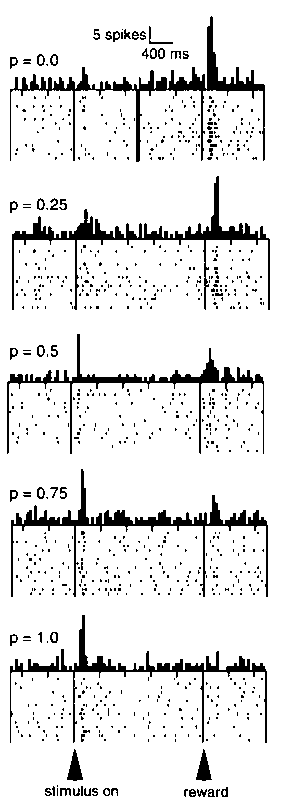
\includegraphics[scale=0.6]{figures/Schultz1.png}
    \hspace{1.5cm}
    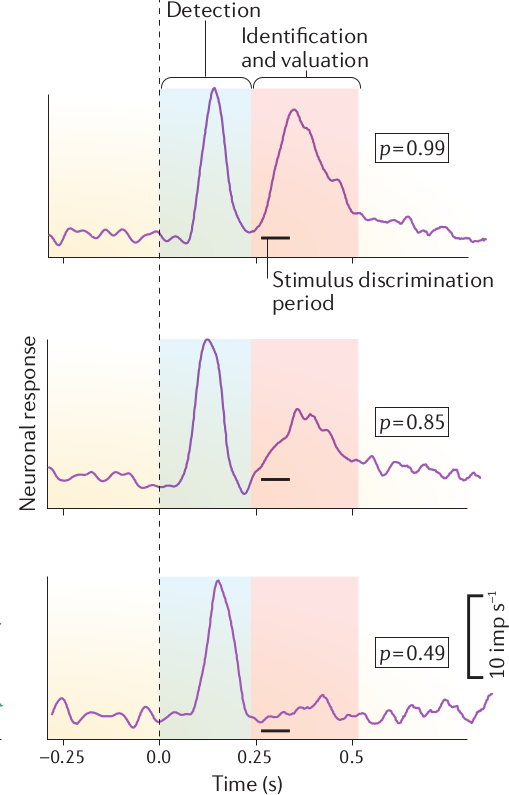
\includegraphics[scale=0.35]{figures/ResponseProbSchultz.png}
    \caption{\textbf{Left:} Adapted from \cite{Fiorillo}: Reward-related responses of dopamine neurons. Distinct stimuli were used to indicate the probability of reward (p increasing from top to bottom). Dopamine neurons signals varied monotonically across the full range of probabilities. At the stimulus onset, the dopamine response increased monotonically as the probability increased; at the reward time instead, the dopamine response decreased monotonically as the probability increased. \textbf{Right:} Adapted from \cite{Schultz2016}: A demanding random dot motion discrimination task reveals completely separated dopamine response components. Larger responses correspond to higher reward probabilities (p). The initial, stereotyped, non-differential activation reflects stimulus detection and decreases back to baseline (blue zone); the subsequent separate, graded increase develops when the animal signals stimulus discrimination; it codes reward value (red zone), which in this case derives from reward probability}
    \label{fig:probDopamine}
\end{figure}
This component reflects the detection of stimulus, regardless its relation with the reward.\\The second component, also called main component or valuation component, defines the function of the dopamine response and reflects the evolving neuronal processing that is required to fully appreciate the value of the stimulus. Thus, at this stage the stimulus is identified and valued. Figure \ref{fig:probDopamine} (right) shows the separation between the detection salience and the valuation component of RPE signals in dopamine neurons.\\Like VTA neurons, VS neurons show as well reward-related response. In monkey experiments first it has been shown that VS neurons predominantly fire in relation to the expectation of reward, regardless of the movement/no-movement reaction (\cite{Schultz1992}). This signals suggested that VS neurons evaluate reward and reward-associated stimuli, and thereby participate in the processing of information underlying the RPE computation.\\The stereotypical responses of striatal projection neurons in VS during learning consist of a sustained increase of activity before the occurrence of the reward delivery (see figure \ref{fig:StriatumN}).
\begin{figure}[H]
    \centering
    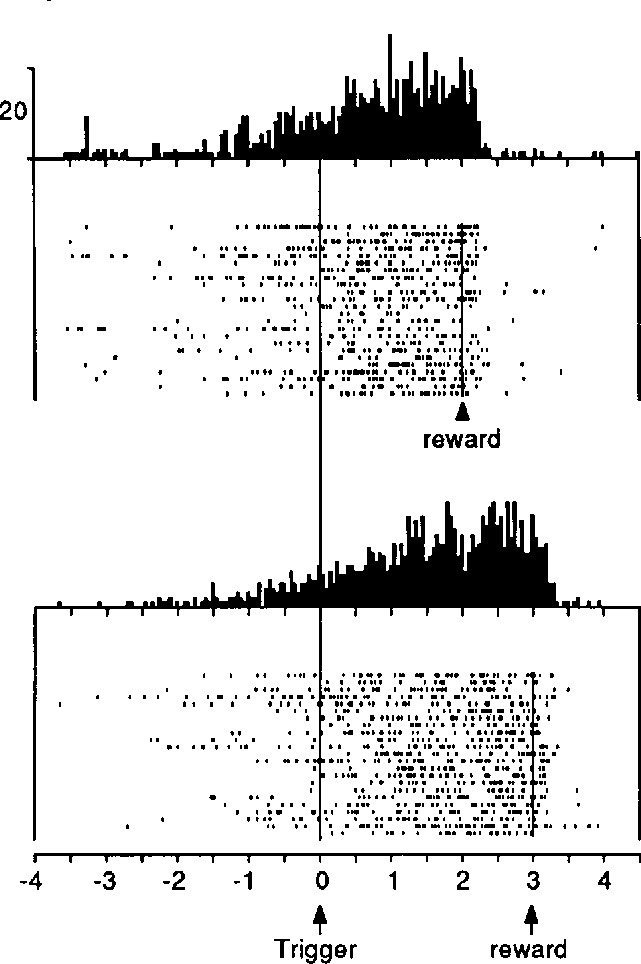
\includegraphics[scale=0.22]{figures/StriatumR.png}
    \caption{Adapted from \cite{Schultz1992}. Stereotypical reward-related VS neuronal activity. Effect of delayed reward delivery in no/ no go task in monkeys. VS neurons show sustained increases of activity before the occurrence of individual task events. VS neurons exhibit activation in relation to the expectation of reward.}
    \label{fig:StriatumN}
\end{figure}
The ventral pallidum (VP), from which neurons with fast spiking activity were recorded, is innervated by dopamine inputs from the midbrain and dopamine directly alters VP neuronal firing (\cite{Napier89}). Since 1991 VP was assumed to integrate reward-related signals carried by VTA dopamine neurons, involved in reward-motivated behavior (\cite{Napier91}). This concept was quickly expanded to encompass the idea that dopamine transmission within the VP regulates a collection of behaviors, including locomotion and cognition (\cite{Napier92}). Contrary to the well-characterized, relatively homogeneous projection neurons dominating striatum, the cellular architecture of VP is only beginning to be understood in terms of their heterogeneous cell-types, neurotransmitters, and connectivity (\cite{Heimer1997}, \cite{Tachibana2012}). In other studies conducted in our lab, it was observed that VP units displayed either purely excitatory, purely inhibitory, or multiphasic excitatory and inhibitory responses to the same stimulus or across reward and unrewarded stimuli (unpublished results). For these reasons, the responses of VP neurons are expected to be diverse among different VP units.\\While there exist an extensive literature on how RPE signals are expressed by single units, how the RPE computations are implemented in VS-VTA neural circuits remains elusive. Thus, better understanding VS-VTA related circuits, will broaden our understanding on the underpinnings of RPE signals.\\In this work I studied the formation of prediction error signals in interregional assemblies during reinforcement. Towards this aim, I used dual site electrophysiological in-vivo data from VS (including ventral pallidum) and VTA, during a reversal go/no go task in mice.\\On this data set I applied a cell assembly detection algorithm (\cite{RussoDurstewitz}). The novel statistical approach was built to detect spike patterns at any time scale and coordination, enabling so the investigation of the time scales and the inter-units lag activation involved in the detected patterns of spikes. I focused the analysis on interregional assembly-pairs, namely assembly formed by two neurons, one in VS and the other in VTA. In this way I were able to examine the directionality between VS-VTA interactions through the inter-unit lag activation.\\I found that, in interregional assembly-pairs, VS predominantly led VTA. Moreover interregional assembly-pairs showed a bimodal time scale distribution, such bimodality was solely present in VS-VTA pairs and did not emerge in intraregional pairs.\\I examined the assembly-pair activity patterns of pairs with different time scales and directionalities. It emerged that different time scales and directionalities segregated different activity patterns. Specifically, in more precise time scale, directional assembly-pairs with VTA following VS showed excitatory responses following reward-predicting stimuli, in agreement with prediction error encoding.\\Taking advantage of neuron types classifications both in VS and VTA, I further investigated the specific cell-type composition of the assemblies exhibiting directionality. Interestingly only assembly-pairs formed by putative striatal projection neurons (pSPN) and dopamine neurons (pDAN) were directional in the direction of VS leading VTA.\\Thus, I looked at the task related activity patterns of different assembly-pair types; and I expected that, being directional, SPN-DAN assembly-pairs could exhibit RPE response.\\Indeed, different assembly-pairs types showed different activity patterns in response to external potentially rewarded stimuli. The segregation reflected different encoding features in different assembly-pair types.\\In particular, SPN-DAN assembly-pairs were mainly activated by the rewarded stimulus, and only a small fraction ($\sim12\%$) was activated by both stimuli. The activation started few hundred milliseconds after the stimulus onset and remained high for few hundred milliseconds ([100,400] ms). SPN-DAN activity pattern suggested that those pairs conveyed the valuation component of RPE signals (\cite{Tobler2003}, \cite{Nomoto2010}, \cite{Schultz2016}). Conversely, FSN-DAN assembly-pairs responded indistinctly to both stimuli, either showing a brief and phasic activation at the stimulus onset or being inhibited by one or both stimuli; these signals suggested that FSN-DAN pairs were involved in motivational and/or hedonic signals. Hence, I put forth the hypothesis that the assembly-pairs specialize in different aspects of the learning-related coding.\\%\\Detailed discussion will be presented in\hyperref[sec:TaskResp]{~Section \ref*{sec:TaskResp}} and\hyperref[sec:FalseAlCorrRej]{~Section \ref*{sec:FalseAlCorrRej}}.\\
So far the description barely considered the dynamic of the learning process. In fact, reward prediction coding signals in dopamine neurons varied according to the probability to get the reward, which was often related to the uncertainty (\cite{Schultz1992}). Dopamine neurons in VTA as well as neurons in VS modified their activity in function to the difference between received and expected outcomes (\cite{Fiorillo}). In similar ways, far from being static, the assembly-pair activity modified itself trial by trial, reflecting the dynamic of the learning.\\This dynamic could not be replicated by the study of activity patterns, for this reason I modeled a reinforcement learning model. Crucial terms of reinforcement learning are the uncertainty of the animal to get the reward and the reward prediction error; the first is high when the animal is unsure about the outcome, and decreases as the animal becomes expert; the latter term reflects the ability of the animal to predict the reward: as the animal learnt is supposed to be able to predict the future outcomes. Both the aforementioned terms were modeled as time evolving components, in such a way that I could take into account the fact that, during the task, the animal had to assign and re-assign new value to the presented stimulus.\\Based on broad knowledge, reward prediction error signals are thought to be anti-correlated with the uncertainty of the animal to get the reward and correlated with the prediction error term of the Rescorla-Wagner models.\\Thus, if SPN-DAN assembly-pairs specifically encoded prediction error signals, I expected their activity to anti-correlate with the modeled uncertainty ($\alpha$) and to correlate with the modeled prediction error ($\delta$).\\Imodeled two linear Poisson regressions and I regressed the assembly-pairs activity on $\alpha$ and $\delta$. Our SPN-DAN assembly-pairs indeed anti-correlated with the uncertainty and correlated with the prediction error term. Furthermore I noted that such correlations were not found in other assembly-pair types, from which I could conclude that SPN-DAN assembly-pairs specifically conveyed reward prediction signals.  
%\chapter{Overview}
\label{chap:Overview}
\section{State of the art}
\label{sec:StateArt}
In this section we present the state of the art of the current knowledge of ventral striatum (VS) and ventral tegmental area (VTA), needed for the study of VS-VTA interaction.\\In VTA, dopamine neurons fire phasically (100-500 ms) after unpredicted rewards or cues that predict reward. Their response to reward is reduced when a reward is fully predicted (\cite{Uchida}). %Furthermore, their activity is suppressed when a predicted reward is omitted. From these observations, previous studies hypothesized that dopaminergic neurons signal discrepancies between expected and actual rewards (i.e., they compute RPE).
The uncertainty about the reward outcome is critical in the measure of information and in assessing the accuracy of predictions. The uncertainty is determined by the probability P to get the reward, and its maximal at $P=0.5$, while decreases at higher and lower probabilities.\\Fiorillo and his collaborators used distinct stimuli indicating the probability of reward, to show that the phasic activation of dopamine neurons varied monotonically across the full range of probabilities (\cite{Fiorillo}). Figure \ref{fig:probDopamine} (left) displays the dopamine neurons response to stimuli with different reward probability. These observations have defined the basis of the current knowledge on dopamine neurons, which are assumed to signal discrepancies between expected and actual rewards, in other words they are thought to compute the reward prediction error (RPE).\\Being essential to learning, since ever RPE signals picked the scientist$'$ curiosity, who dissected the evolution in time of those signals to understand the underlying nature of multiple time components of RPE. Several studies have shown that RPE signal evolves in time from unselective sensory detection to more demanding and crucial stages of identification and valuation (\cite{Tobler2003}, \cite{Nomoto2010}, \cite{Fiorillo2013}, \cite{Schultz2016}), value that is constantly adapted during the learning process by dopamine neurons (\cite{Tobler2005}). The initial component, characterized by a brief activation, occurs unselectively in response to a large variety of unpredicted events and corresponds to the large range and heterogeneous nature of potentially rewarding stimuli and object present in the environment. This component reflects the detection of stimulus, regardless its relation with the reward.\\The second component, also called main component or valuation component, defines the function of the dopamine response and reflects the evolving neuronal processing that is required to fully appreciate the value of the stimulus. Thus, at this stage the stimulus is identified and valued. Figure \ref{fig:probDopamine} (right) shows the separation between the detection salience and the valuation component of RPE signals in dopamine neurons. %In stark contrast to the simple models proposed previously, we observed that information about reward and expectation is distributed among multiple brain areas and already mixed in many individual input neurons. Our data suggest that the RPE computation is not a one-step process combining pure information about reward and expectation in dopamine neurons. Nor do dopamine neurons receive complete RPE from a specific brain area. Instead, the coexistence of input neurons encoding pure and mixed information, some of which are partial and complete RPE signals, appears to be a sign of redundant computations distributed in a complex neuronal network that ultimately converge onto dopamine neurons to construct a more complete RPE signal.
\begin{figure}[H]
    \centering
    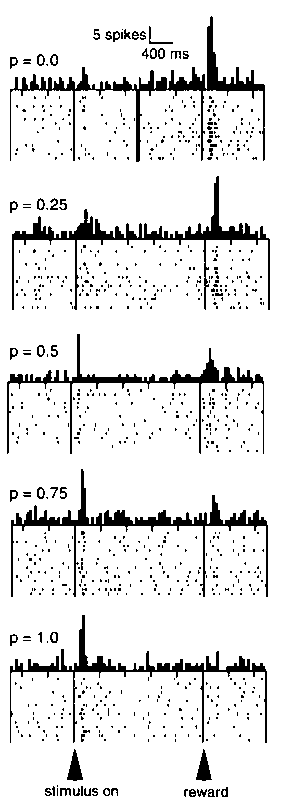
\includegraphics[scale=0.6]{figures/Schultz1.png}
    \hspace{1cm}
    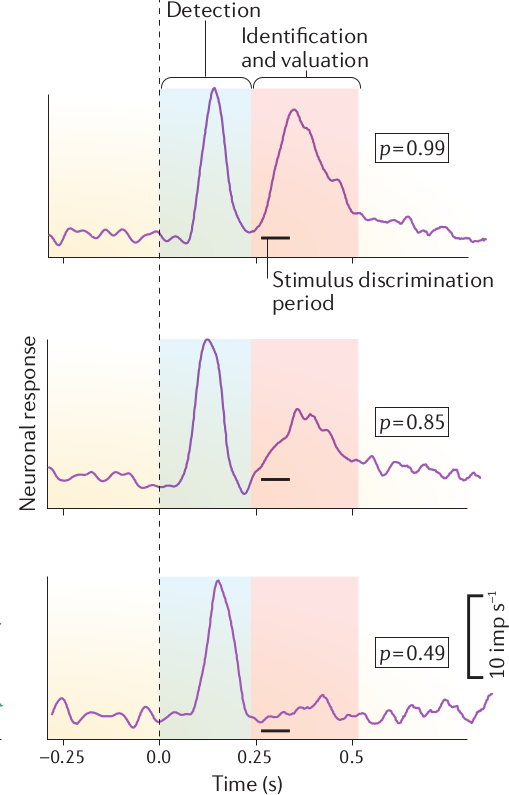
\includegraphics[scale=0.35]{figures/ResponseProbSchultz.png}
    \caption{\textbf{Left:} Adapted from \cite{Fiorillo}. Reward-related response of dopamine neurons. Distinct stimuli were used to indicate the probability of reward (P increasing from top to bottom). Dopamine neurons signals varied monotonically across the full range of probability. At the stimulus onset the dopamine response increased monotonically as the probability increased, at the reward time instead the dopamine response decreased monotonically as the probability increased. \textbf{Right:} Adapted from \cite{Schultz2016}. A demanding random dot motion discrimination task reveals completely separated dopamine response components. Higher response corresponds to higher reward probability (p). The initial, stereotyped, non-differential activation reflects stimulus detection and decreases back to baseline (blue zone); the subsequent separate, graded increase develops when the animal signals stimulus discrimination; it codes reward value (red zone), which in this case derives from reward probability}
    \label{fig:probDopamine}
\end{figure}
%\begin{figure}
 %   \centering
  %  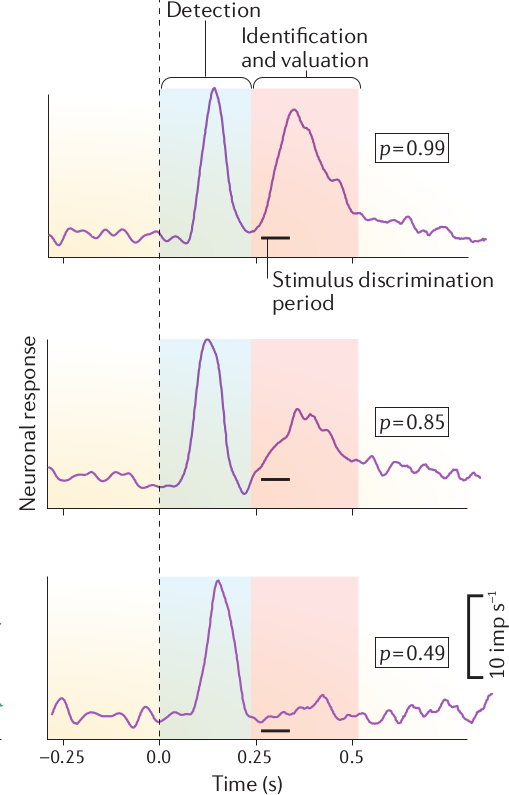
\includegraphics[scale=0.4]{figures/ResponseProbSchultz.png}
   % 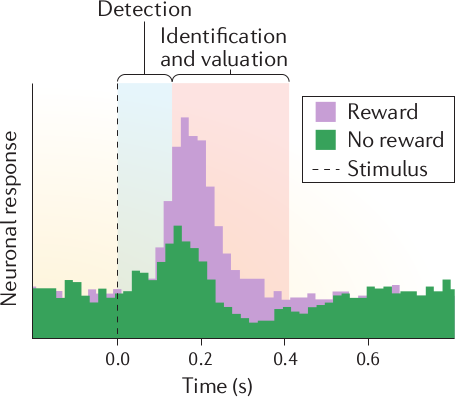
\includegraphics[scale=0.4]{figures/Schultz2016CSMod.png}
  %  \caption{Adapted from \cite{Schultz2016}. A demanding random dot motion discrimination task reveals completely separated dopamine response components. Higher response corresponds to higher reward probability (p). The initial, stereotyped, non-differential activation reflects stimulus detection and decreases back to baseline (blue zone); the subsequent separate, graded increase develops when the animal signals stimulus discrimination; it codes reward value (red zone), which in this case derives from reward probability}
 %   \label{fig:probSchultz}
%\end{figure}
Like VTA neurons, VS neurons show as well reward-related response. In monkey experiments first it has shown that VS neurons predominantly fire in relation to the expectation of reward, regardless the movement no-movement reaction (\cite{Schultz1992}). This signals suggested that VS neurons have access to central representations of reward and thereby participate in the processing of information underlying the RPE computation.\\The stereotypical response of projection neurons in VS during learning consists in a sustained increase of activity before the occurrence of the reward delivery (see figure \ref{fig:StriatumN}).
\begin{figure}[H]
    \centering
    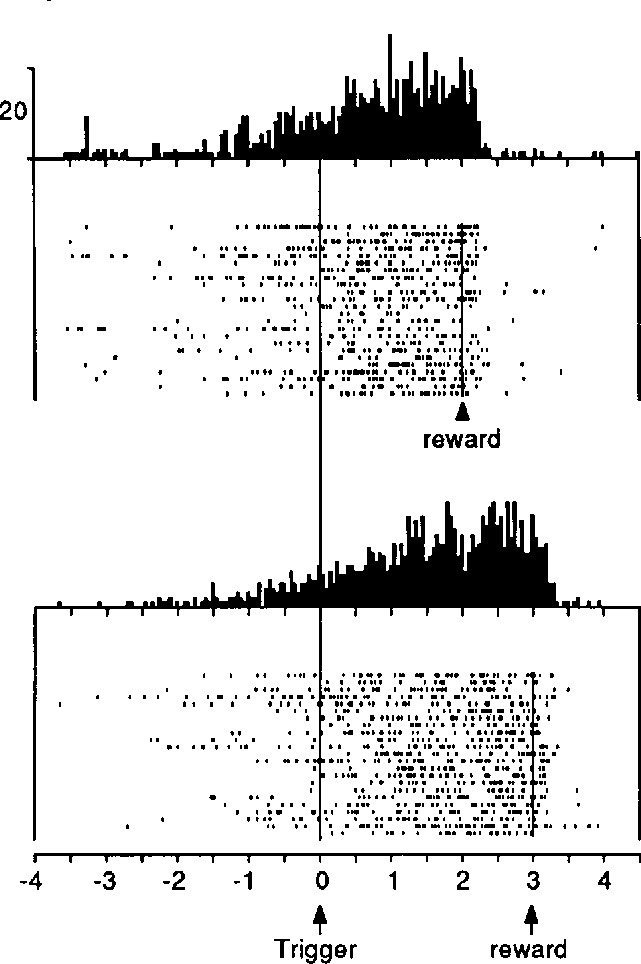
\includegraphics[scale=0.22]{figures/StriatumR.png}
    \caption{Adapted from \cite{Schultz1992}. Stereotypical reward-related VS neuronal activity. Effect of delayed reward delivery in no/ no go task in monkeys. VS neurons showed sustained increases of activity before the occurrence of individual task events. VS neurons exhibit activation in relation to the expectation of reward.}
    \label{fig:StriatumN}
\end{figure}
The ventral pallidum (VP), from which we recorded fast spiking activity, is innervated by dopamine inputs from the midbrain and dopamine directly alters VP neuronal firing (\cite{Napier89}). Since 1991 VP was assumed to integrate reward-related signals carried by VTA dopamine neurons, involved in reward-motivated behavior (\cite{Napier91}). This concept was quickly expanded to encompass the idea that dopamine transmission within the VP regulates a collection of behaviors, including locomotion and cognition (\cite{Napier92}). Contrary to the well-characterized, relatively homogeneous projection neurons dominating striatum, the cellular architecture of VP is only beginning to be understood in terms of their heterogeneous cell-types, neurotransmitters, and connectivity (\cite{Heimer1997}, \cite{Tachibana2012}). In other studies we observed that VP units displayed either purely excitatory, purely inhibitory, or multiphasic excitatory and inhibitory responses to the same stimulus or across reward and unrewarded stimuli (unpublished results). For these reason, the responses of VP neurons are expected to be diverse among different VP units, probably depending on the involvement of the unit in a specific coding.
\section{Experiment and data set}
\label{sec:Dataset}
In this session we describe the experiment and the collected data for the analysis in object in this work. The experiment and the single units classification was conducted by Max Scheller, medical student, member of the Kelsch group.\\The task presented is a go/no-go reversal odor discrimination task (see details in \hyperref[sec:MatAndMet]{~Section \ref*{sec:MatAndMet}}).
\begin{figure}[H]
    \centering
    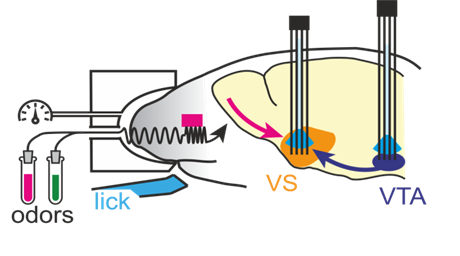
\includegraphics[scale=0.92]{figures/Experiment.png}
    %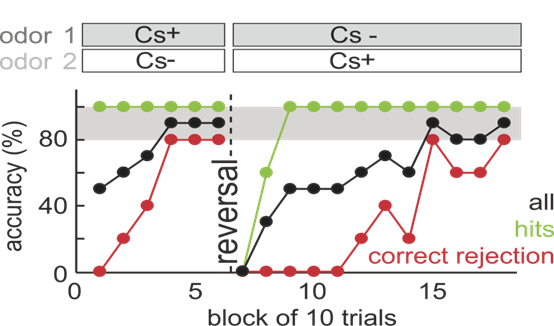
\includegraphics[scale=1]{figures/Performance.png}
    \caption{Scheme of the experimental setup. Two odors in randomized sequences were presented, the mouse was head-fixed and, to get the reward, had to lick during the allowed licking period when the rewarded odor was presented. Electrodes were implanted in VS (specifically olfactory tubercle -OT-)/VP  and VTA to record the neural activity.}
    \label{fig:experiment}
\end{figure}
In figure \ref{fig:experiment} the scheme of the experimental set-up. Dual-site in-vivo data were recorded in VS (specifically olfactory tubercle -OT-), including VP, and VTA, meanwhile two odors were presented to head-fixed mice, one rewarded (CS+) with reward probability 0.9, the second one unrewarded (CS-). Learning the task consisted in licking at least a defined number of times (two or three depending on the paradigm) during a specific interval, called lick window, when the rewarded odor (CS+) was presented (hit trials) and not licking when unrewarded odor (CS-) was presented (correct rejection trials). Whereas a bad performance consisted in not licking, or licking outside the lick window period, at CS+ presentation (miss trials), or licking at CS- presentation (false alarm trials). Once the performance criterion was reached, the contingencies were switched, in other words the rewarded odor became unrewarded and vice-versa. Once the performance criterion was reached also in the reversal phase the extinction phase followed, in which neither one of the two odors was rewarded. The lick window was open for an interval of a duration ranging between 1500 ms and 2000 ms depending on the paradigm, and it was open only after a delay that could range from 500 ms to 1500 ms. Only licks happening in the lick window interval were counted as valid to get the reward. Figure \ref{fig:performance} displays one example of performance in hit, correct rejection trials and overall.
\begin{figure}[H]
    \centering
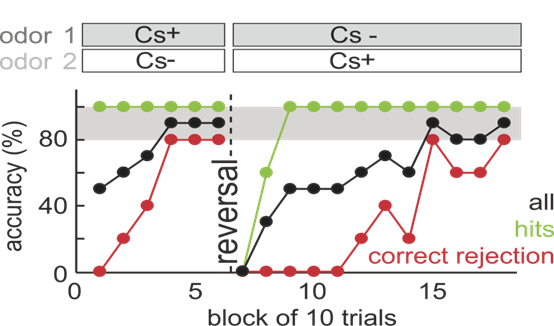
\includegraphics[scale=0.8]{figures/Performance.png}
\caption{Example of the performance of one animal in original and reversal phase. In the shown paradigm the performance criterion to be reached to switch to the reversal phase was $79\%$, meaning that this level of accuracy had to be satisfied for hit trials and correct rejection trials. Black line indicates global performance including hit trials and correct rejection trials. Green line is the performance for the performance in hit trials and red lines is the performance in correct rejection trials.}
\label{fig:performance}
\end{figure}
\section{Materials and Methods}
\label{sec:MatAndMet}
\textbf{Data acquisition.} Recordings were performed with two Intan 64 channel RHD 2164 miniature amplifier boards connected to a RHD2000 interface board and open-source Intan interface software. Inputs from the laser, olfactometer and sniff sensor were simultaneously recorded with the same interface board, as were reward application and licking activity (via an infra-red beam break sensor positioned in front of the licking spout, Omron Electronics EE-SX3009-P1). Data were sampled at 30 kHz.\\\textbf{Probe Design.} For the recordings during reversal learning, the OTu was targeted with 16 tetrodes per array and for the DA plasticity experiment each array contained up to 32 tetrodes. Given the relatively high distance ($>6$ mm) between sites, depth of the target structures ($>5$ mm) and curvature of the OT/VP, Max Scheller and his collaborators developed a probe design specifically attuned to these challenges and easily adaptable to different single- or multi-site configurations. A detailed tutorial for the streamlined successor version of the implant used here is in preparation. The design exploits the high precision of the mature production technology of printed circuit boards (PCB)  ($\pm10\mu$ m, custom-designed boards ordered from Wuerth Electronics) to achieve a precise x-y-placement of the guiding channels for optical fibers (Thorlabs \#) and tetrodes (spun from 12.5 $\mu$m teflon-coated tungsten wire, California Fine Wire). For the VTA, four tetrodes were attached to an optical fiber and fixed in their guiding channel. For the OT/VP, the implant was placed above a mould of the ventral brain surface, and tetrodes and an optical fiber were advanced to their z-position and fixed in place, matching the bowl-shaped 3d-curvature of the OT (see figure \ref{fig:implant}). Single tetrode wires were attached to the PCB using gold pins (Neuralynx). The connection between PCB and head stage was made via a Molex SlimStack connector (mated height: 1 mm, pitch: 0.4 mm, 70 channels, \# $502426-7030$) and an custom adaptor to the 2x36 Omnetics Nano Strip connectors of the Intan RHD2164 head stage.\\ 

\begin{figure}[H]
    \centering
    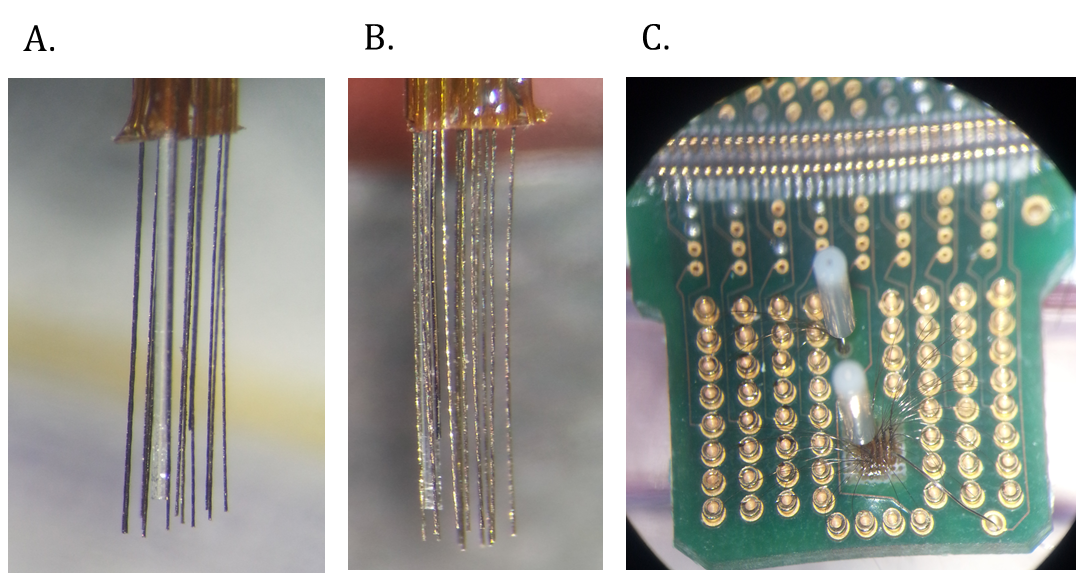
\includegraphics[scale=0.4]{figures/Implant.png}
    \caption{Photo provided by Max Scheller.\textbf{A., B.} Lateral and frontal view of OT implant. \textbf{C.} Finished implant without protective epoxy cap (top view).}
    \label{fig:implant}
\end{figure}
\textbf{Animals and surgery details.}
18 adults mice (DAT:Cre$+$, ChR2:YFP$+$ ) (5-6 months aged) were implanted. The surgery duration was less than 2 hours, after which mice were housed individually. The recovery period was one week.\\ After completion of the experiments, animals were euthanized and perfused with 4$\%$ Paraformaldehyde (PFA) solution. Placement of tetrodes in the target areas was evaluated post mortem by first explanting the whole brain, dorsal skull and attached probe as a unit, documenting the ventral aspect, where tetrode tips could be seen through the surface of the OT (photo \ref{fig:surgery}, left), and, in some cases, breaching it (photo \ref{fig:surgery}, right). After that, the relevant hemisphere was sectioned (100 $\mu$m) sagittally with a microtome and mounted serially, so tetrode tracks could be traced.\\
\begin{figure}[H]
    \centering
    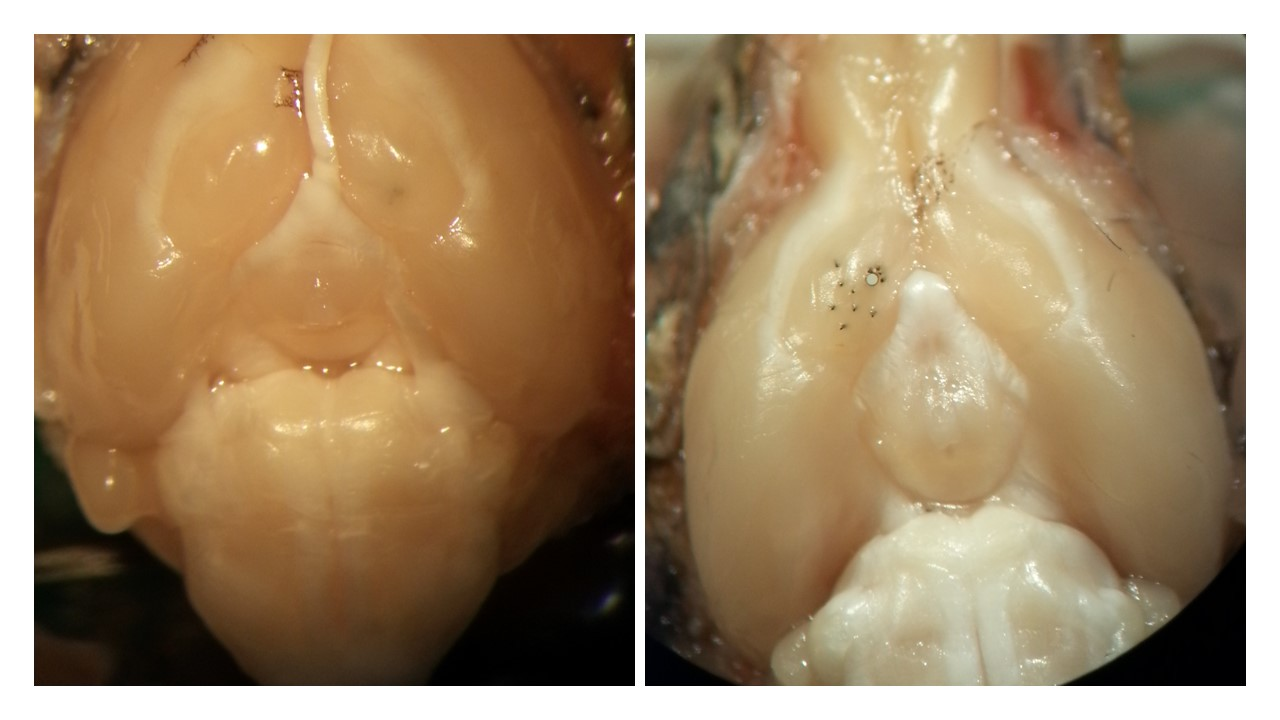
\includegraphics[scale=0.2]{figures/surgery_3.jpg}
    %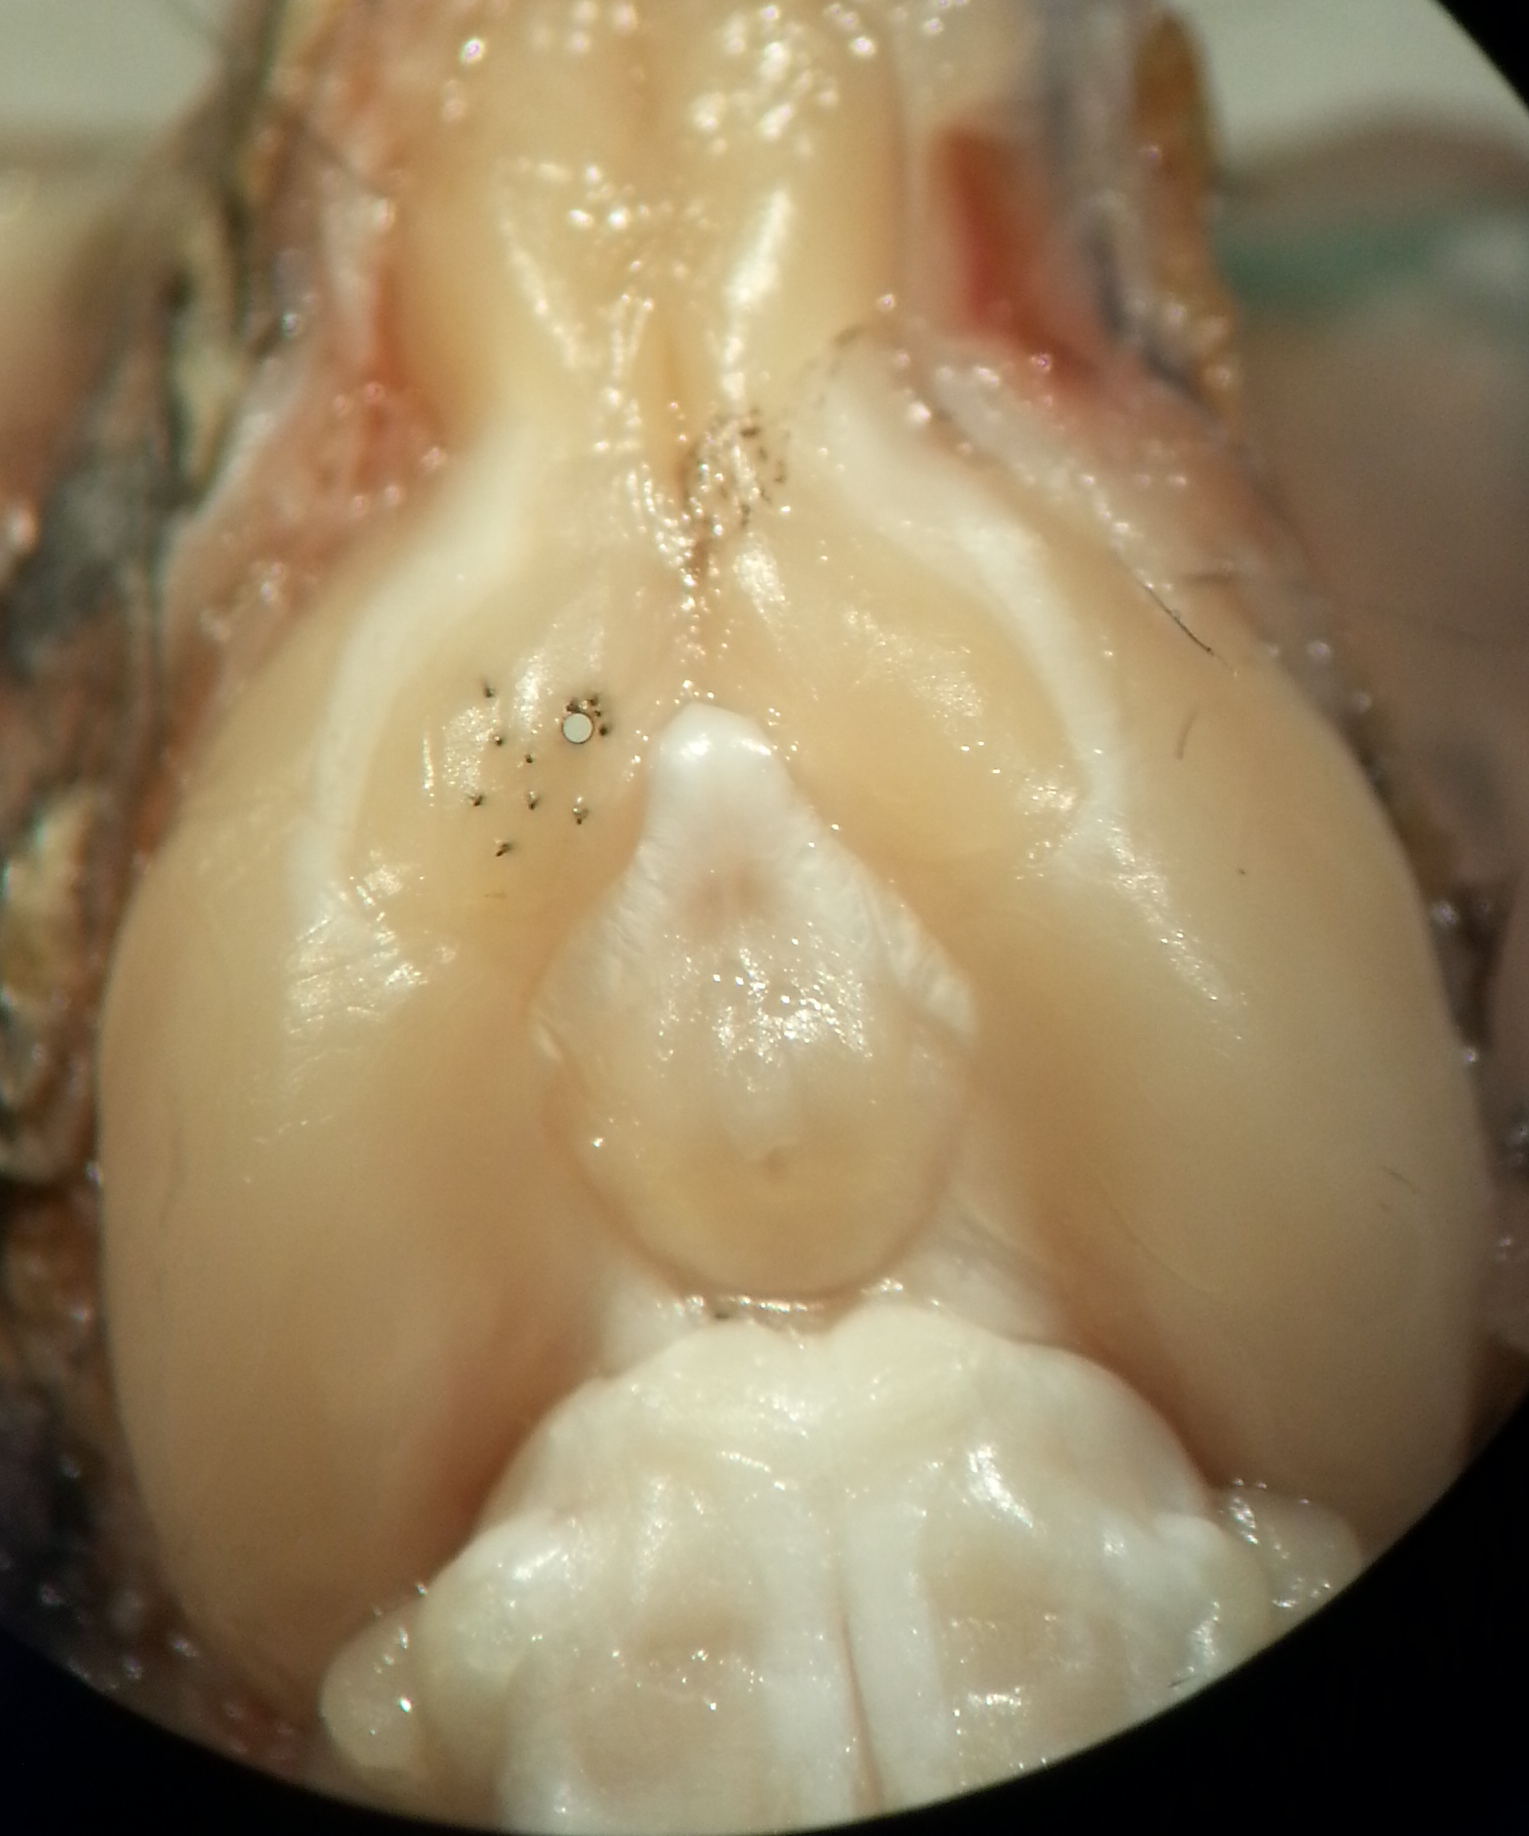
\includegraphics[scale=0.1]{figures/Surgery2.png}
    \caption{Photo provided by Max Scheller. Post mortem photos to evaluate the placement of tetrodes in the target areas. First the the whole brain, dorsal skull and attached probe as a unit were explanted. Then tetrode tips could be seen through the surface of the OT (photo\ref{fig:surgery}, left), and, in some cases, breaching it (photo\ref{fig:surgery}, right).}
    \label{fig:surgery}
\end{figure}
\textbf{Behavioral conditioning in the go/no-go task.} We trained the animals in the head-fix setup described above. Mice received water in their home cage so that their body weight stabilized at 85$\%$ of baseline body weight. The training comprised multiple stages and progressed after reaching a performance criterion defined as at least 80$\%$ correct responses in 50 consecutive trials. Trials were considered correct if either at a go-response the reward was retrieved or at a no-go-response no significant licking was detected during the lick window. In the initial sessions, the animals’ licking behavior was shaped by first presenting them with a drop of water and subsequently letting them obtain more water when they licked at the licking spout (available in a random interval schedule, 0.5-12 seconds). Stage 1 (training): A single odor (1.5 s stimulus duration) was presented. Animals could obtain a 5 $\mu l$ drop of water if they licked at least three times during a window from 0 to 2.5 s after stimulus onset (retrieval window), this was considered a go-response. The interval between trials was randomly set at $10\pm 2$ s in all stages. Stage 2 (discrimination) consisted of two odors in pseudo-random succession (no more than 3 consecutive trials with the same stimulus). One odor (1.5 s duration) was rewarded as in stage 1 (retrieval window: 0.5 - 2.5 s), while a go-response for the second odor was registered as a false alarm and thus incorrect. No punishment was used. Stage 3 (reversal learning) used the same parameters as stage 2, but upon reaching the performance criterion (in the original phase), the reward contingency of the odors was switched (reversal phase). The data set used in this study consisted of one reversal learning session per animal.\\% (10 sessions with a total yield of 75 single units) after we accustomed them gradually to a longer lick delay (1.5 – 3 s), keeping odor delivery concurrent (3 s duration). 
\textbf{Data pre-processing: Spike detection.} To reduce noise and movement artifacts affecting all recording sites, we subtracted the median voltage trace of all channels from each recorded trace. The resulting signal was band pass filtered between 300 and 5000 Hz (4th order Butterworth filter, built-in MATLAB function). A threshold value for spikes was computed as a multiple (7.5x) of the median absolute deviation of the filtered signal (\cite{Quiroga}). Temporally proximal detected peaks over threshold were pruned by height to a minimum distance of 1 ms to avoid multiple detections of the same multiphasic spike. When an event was detected on multiple channels of a tetrode, the timestamp of the highest detected peak was used. Spike waveforms were extracted around $-10$ to $+21$ samples around the peak.\\
\textbf{Data pre-processing: Spike sorting.} Spike sorting was done with a custom-built graphical user interface in MATLAB, originally developed by A. Koulakov (CSHL). Metrics used for clustering included detected peak height or amplitude (and the respective principal components over channels), and the first three principal components of the waveforms for each respective channel when a spike was predominantly recorded on one channel. The quality of single unit clusters was assessed using the mlib toolbox by Maik Stuettgen (Vs. 6, $\href{https://de.mathworks.com/matlabcentral/fileexchange/37339-mlib-toolbox-for-analyzing-spike-data}{MLIB-toolbox-for-analyzing-spike-data}$) with particular attention to peak height distribution (fraction of lost spikes due to detection threshold), contamination (fraction of spikes during the refractory period $<5ms$) and waveform variance.\\
%For analysis of the silicon probe data, spike detection and spike sorting was done using KiloSort (\cite{Pachitariu}), followed by manual curation with Phy (\href{https://github.com/kwikteam/phy}{KiloSort}) using similar parameters to assess unit quality.\\
\textbf{Data pre-processing: Inclusion criteria of units.} For further analyses, units were only included if they complied with a set of criteria: Throughout the analyzed part of the recording session units were allowed to only have a maximum change in baseline firing rate from beginning to the end of the session of less than ten percent and intermittent maximum fluctuations of 20$\%$.\\ After exclusion of the first ten trials of odor application where we frequently observed an initial response habituation, both odor responses had to be stable throughout the $'$pre$'$ phase.\\\textbf{Optogenic tagging.}Identification of optogenetically modulated units was achieved by crosscorrelation of spike train and laser pulses.\\After sessions, trains of 5 ms laser pulses (8-12 Hz, 5 mW) were delivered in either brain region via the implanted optical fibers. For each unit/region-pair, a test crosscorrelogram was computed from the timestamps of spikes and laser pulses (bin width: 1 ms, lag:  0-20 ms). To test for significant modulation, control crosscorrelograms ($n = 10000$) were constructed by shifting each laserpulse randomly in the interval $\pm$30 ms around its original time, thus destroying any temporal relation on that timescale while preserving the properties of the spike train. Modulation was considered significant if two consecutive bins of the test crosscorrelogram lay outside of the middle 95$\%$ of the global distribution in the control crosscorrelograms. 

%
\section{Single cells analysis}
\label{chap:UnitsAnalysis}
{\color{red} Not Stable paragraph}
The aim of the project is to understand the nature of interactions between ventral striatum (VS) and ventral tegmental area (VTA). Loops and circuit effects make puzzling to understand the whole picture of the aforementioned interactions (figure\ref{fig:Brain}, left). To see how specific interactions are involved in the prediction coding is needed a cell-types classification of underlying units.\\
In this chapter we present the cell types classification provided by Max Scheller.
\begin{figure}
    \centering
    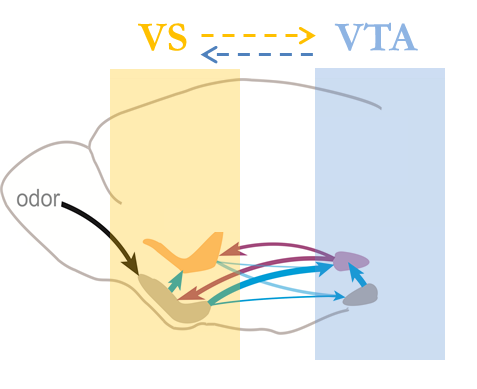
\includegraphics[width=0.45\textwidth]{BrainVSVTA.png}
    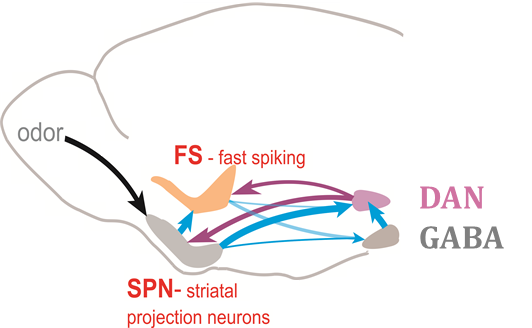
\includegraphics[width=0.45\textwidth]{Brain.png}
    \caption{Schematic illustration of VS-VTA regions and their interactions in mice brain. On the left the mesoscopic vision, VS in yellow is subdivided in Odor Tuberculum (OT) and Nucleus Accumbens (NAcc), neurons of VS project and receive inputs to/from VTA. On the right the detailed vision, with specification of the recorded cell-types involved in VS-VTA circuit.}
    \label{fig:Brain}
\end{figure}
The data-set included $803$ VS and pallidal units and $272$ VTA units in total, that were classified in sub-types. Specifically VS units were classified as either striatal projection neurons (SPNs), fast-spiking neurons (FSNs) or cholinergic interneurons(CINs), according to their firing pattern characteristics computed using only spikes during the inter-trials interval and after session. Units with a firing rate higher than $12 Hz$ were assigned as FSNs and all units with a firing rate below $2 Hz$ as SPNs. Units in the remaining range were designed as putative regular-firing CINs if the coefficient of variation (CV) of their $ISI$ distribution was less than $1.2$ and ISIs less than $60 ms$ contributed no more than $20\%$ of all ISIs (\cite{Inokawa}). Finally the resting units were characterized as SPNs or FSNs if they ever were silent for more than $2s$ (\cite{Graybiel}). Using this classification mean normalized autocorrelations and mean waveforms have canonical patterns.\\ The VS consists of the nucleus accumbens and the olfactory tubercle (OTu).
Considering the close anatomical relationship between OT and VP (\cite{Heimer1982}) and the statistics of cell types in the two regions (FSNs in striatum represent only $<5\%$ of the population({\color{red}askfor paper to cite}), while pallidal units have higher firing rate ({\color{red}askfor paper to cite}), it can be assumed that the recorded FSNs are pallidal neurons.\\
VTA units were instead classified as dopaminergic neurons (DAN), gabaergic units (GABA), and glutamatergic neurons (GLU) according to their task related activity using a clustering approach adapted from (\cite{Uchida}). First, response were characterized for the relevant time spans ({\color{red}ask Max for the updated intervals}(CS+ from 0 to 0.5 and US from -0.5 to 0 and from 0 to 0.5), significant task related response were assessed with Friedman test, and only significant units ($p<0.05$) were included in the clustering classification ($~80\%$ of units).\\For the clustering of US-responsive units, the spike count distribution were used to construct one trace per neuron by computing aurROC-values analogously to the Friedman significant test, yielding a trace of values between 0 and 1. Where 0.5 means no distinguishability between test and control distribution. Hierarchical clustering was done on these traces using the in-built linkage matlab function.
\begin{figure}
  \centering
    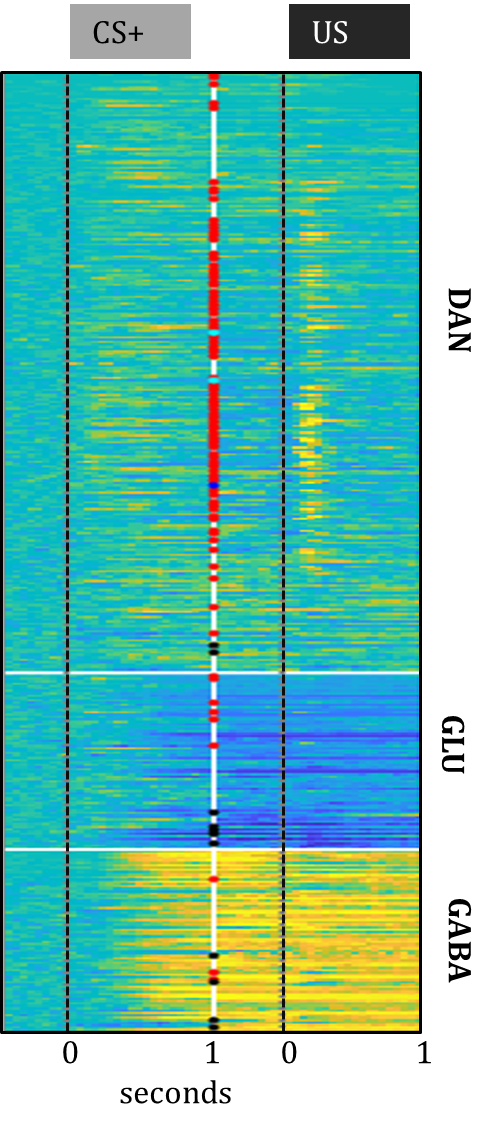
\includegraphics[scale=0.75]{figures/ClassificationUnits.png}
   \caption{Figure provided by Max Scheller. VTA classification according to units task related activity using a clustering approach adapted from (\cite{Uchida}). In this study we focused on dopaminergic and gabaergic units in assemblies. Dopaminergic units show a phasic response to the reward, whereas gabaergic units are tonically active neurons.}
    \label{fig:ClassificatonVTA}
\end{figure}
Considering the units recorded in paradigms used for the assembly analysis, the cell-types result to occur in VS and VTA as shown in figure\ref{fig:PieRegions}.
\begin{figure}
  \centering
    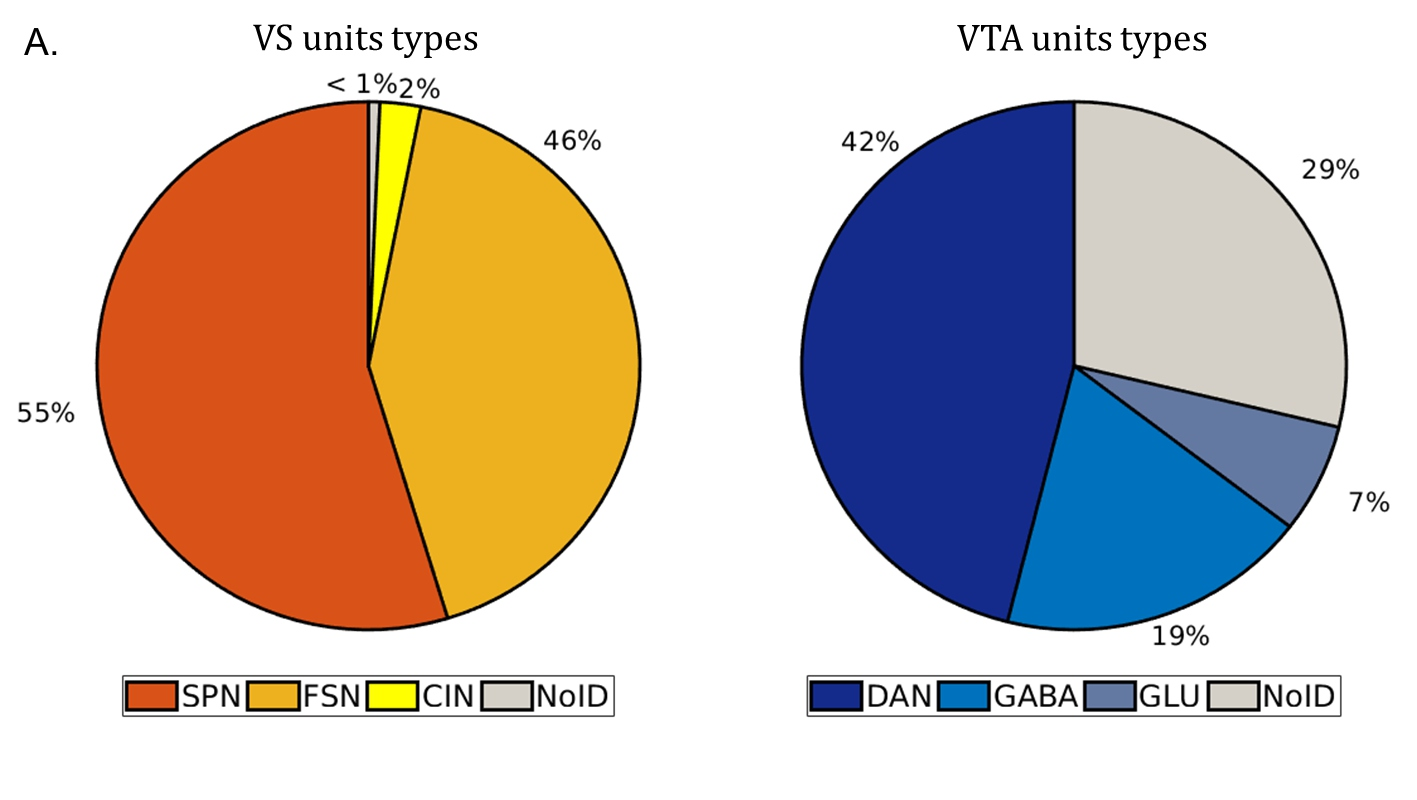
\includegraphics[scale=0.5]{figures/PieRegions1.pdf}
   \caption{Left: units types pie chart in ventral striatum. Right: units types pie chart in ventral tegmental area}
    \label{fig:PieRegions}
\end{figure}


%\chapter{Cell assembly detection method}
\section{Introduction}
\section{Method}
%\section{Possible application on real data}
%\chapter{Cell assembly analysis}
\label{chap:AssemblyAnalysis}
In this chapter we present the assembly analysis conducted on the data set introduced in \hyperref[chap:Dataset]{Chapter~\ref*{chap:Dataset}}, using the cell assembly detection algorithm and the single units classification presented in \hyperref[chap:AssemblyMethod]{Chapter~\ref*{chap:AssemblyMethod}} and \hyperref[chap:UnitsAnalysis]{Chapter~\ref*{chap:UnitsAnalysis}} respectively.\\
The cell assembly detection algorithm is designed to detect any coordinated spike trains patterns at any time scale. The time scales are explored running over different bin-widths. Further we examined the lag distribution. Lags describe the temporal distance in activation between units in assembly. Applying the cell-assembly algorithm we detected synchronous ($lag=0$) and asynchronous ($lag\neq0$) cell assemblies at arbitrary time scale ($\Delta$).\\
We were interested in cross areal interactions and directionality between Ventral Striatum (VS) and Ventral Tegmental Area (VTA).  Inter-regional assembly-pairs are assemblies formed by two neurons, of which one neuron is located in  the VS and the other one in VTA. At the pair-level, the lag in activation between units in assembly indicates the lag in activation between the two regions. A positive lag ($lag>0$) indicates that the VS unit is preceding in its activation the VTA unit, or in other words: VS is leading and VTA is following. A negative lag ($lag<0$) means that the VTA unit is preceding the activation of the VS unit, hence VTA is leading and VS is following.
\section{Cell types occurrence}
Based on the unit classification (\hyperref[chap:UnitsAnalysis]{Chapter~ \ref*{chap:UnitsAnalysis}}), inter-regional assembly were classified according to their underlying cell-types (fig.\ref{fig:PieAssembliesTot} (B.)).
Comparing the two pie charts related to the VS region, one observes fast spiking neurons (FSN) occur in inter-regional pairs more often than striatal projection neurons (SPN) (fig.\ref{fig:PieAssembliesTot} (B.-left)), even though recorded FSN are less than recorded SPN (fig.\ref{fig:PieAssembliesTot} (A.-left)).
\label{sec:CellTypesOcc}
\begin{figure}[H]
    \centering
    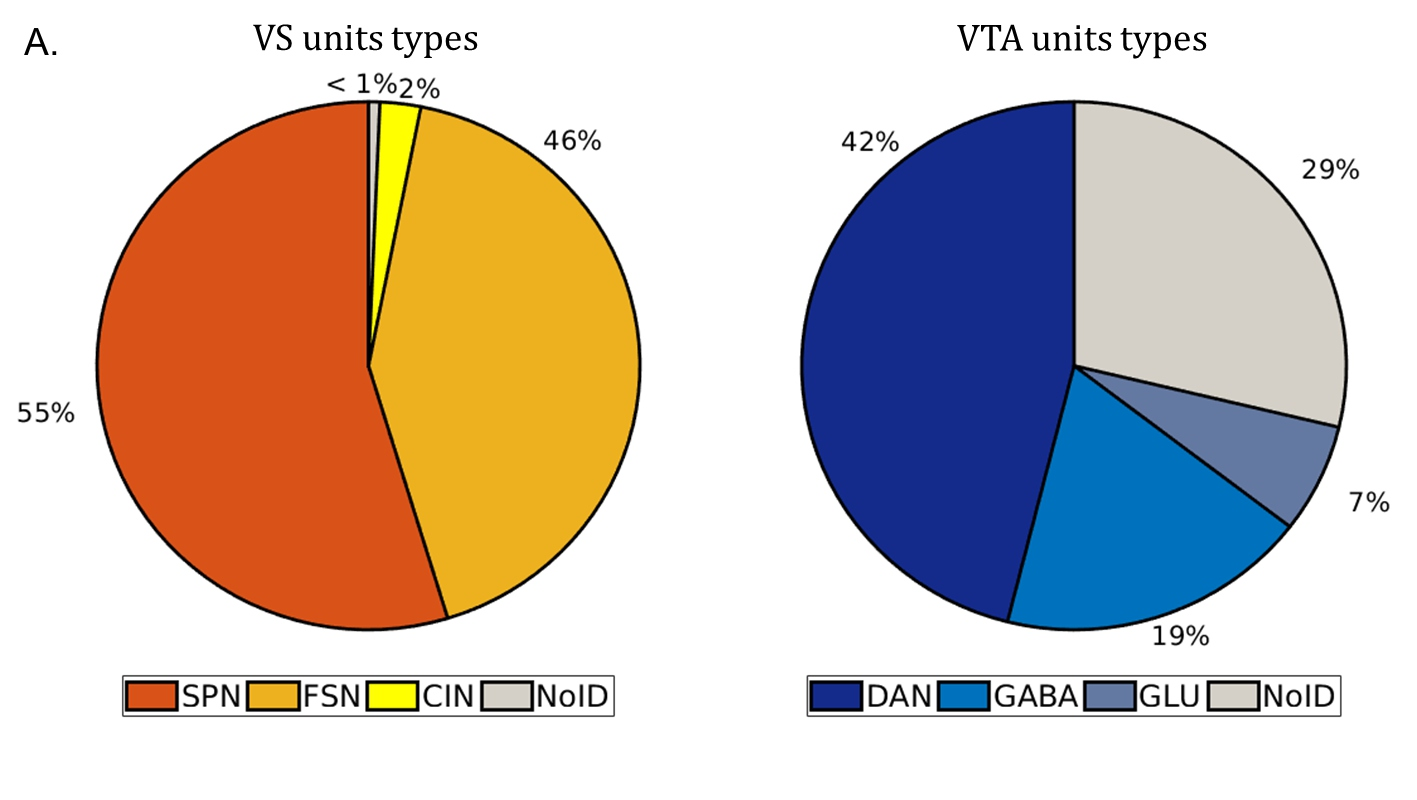
\includegraphics[scale=0.33]{figures/PieRegions1.pdf}
    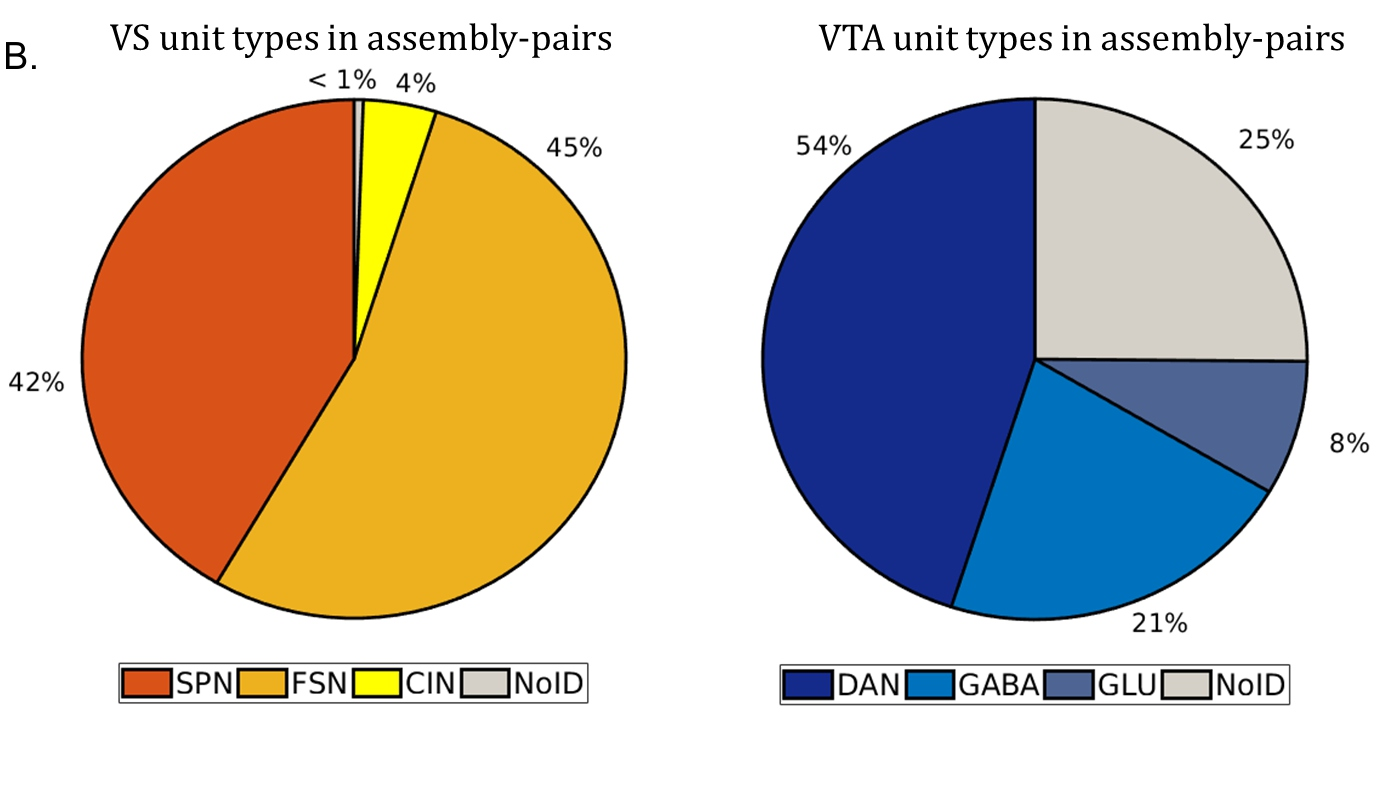
\includegraphics[scale=0.33]{figures/PieAsNotAs.pdf}
    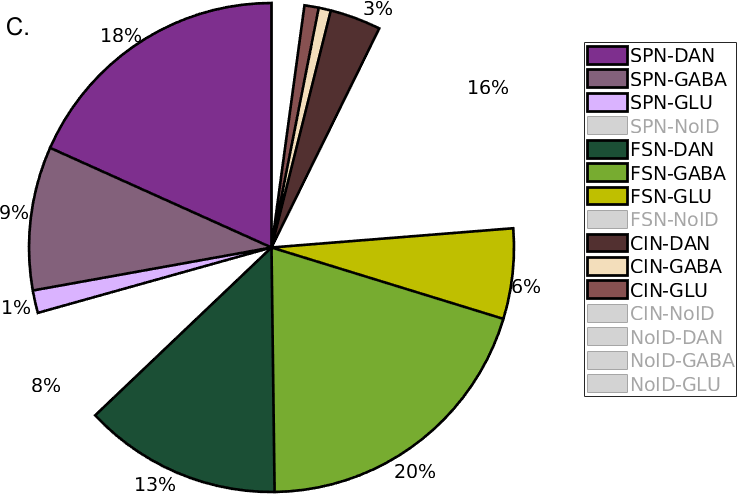
\includegraphics[scale=0.33]{figures/PieAssembliesTot1.png}
    \caption{(A.) Occurrence of classified and not classified units in VS and VTA. (B.) Occurrence of classified and not classified units of VS and VTA in inter-regional assembly-pairs. In VS, FSN occur in inter-regional pairs more often than SPN, even though more SPN than FSN were recorded.(C.) Pie charts of assemblies types. Not indicated percentage are $<1\%$. Missing pieces of cake indicates pairs that include not classified units. The four more represented inter-regional pairs, including only classified units, are pairs between fast spiking and gabaergic neurons ($20\%$), striatal projection neurons and dopaminergic neurons ($18\%$), fast spiking and dopaminergic units ($13\%$) and striatal projection and gabaergic units ($9\%$). }
    \label{fig:PieAssembliesTot}
\end{figure}
We hypothesize that the formation of inter-regional asemblies  depended on the cell-types; to verify this hypothesis we conducted for each of the two regions a Pearson's $\chi^2$ test. Of the classified unit types, only the ones detected at sufficient frequencies could tested for reasons of statistical power: namely putative striatal projection neurons (pSPN) and fast spiking neurons (FSN) in VS, and dopaminergic and gabaergic units in VTA. Only few striatal cholinergic interneurons and VTA glutamatergic units were detected are poorly represented in the examined data-set, and in the entire work and therefore not amenable to statistical analysis. We therefore focused on the four most prominent neuron types and the cell assembly pairs formed between those units.\\Whether the recorded unit may or may not be part of an inter-regional pair is described  in the contingencies tables \ref{tab:chi2_asnotasVS}, \ref{tab:chi2_asnotasVTA}. In the contingencies tables, the number (compared to the expected values indicated in parentheses) of specific cell types in inter-regional pairs were reported with $\chi^2$ statistic p-values. For each test the $\alpha$ significance level was fixed at $0.05$, unless otherwise specified.
\begin{table}[H]
    %\centering
\begin{tabular}{ |p{3cm}|p{3cm}|p{3cm}| }
 \hline
 \multicolumn{3}{|c|}{Pearson$'$s $\chi^2$ test VS unit type and inter-regional pair relationship} \\
 \hline
 & In pairs & Not in pairs\\
 \hline
 SPN & 153 (197.64) & 253 (208.36) \\
 \hline
 FSN & \textbf{197 (156.36)} & 116 (164.64)\\
 \hline
 \multicolumn{3}{|c|}{$\chi^2$ statistic  45.13}\\
 \multicolumn{3}{|c|}{p-value = $1.8\times10^{-11}$}\\
 \hline
 \multicolumn{3}{|c|}{$\chi^2$ statistic Yates correction 44.12}\\
 \multicolumn{3}{|c|}{p-value = $3.1\times10^{-11}$}\\
 \hline
\end{tabular}
\caption{Pearson's $\chi^2$ contingency table with $\chi^2$ value and p-value. Unit-types and inter-regional pairs formation are correlated in Ventral Striatum.}
\label{tab:chi2_asnotasVS}
\end{table}
\begin{table}[H]
    %\centering
\begin{tabular}{ |p{3cm}|p{3cm}|p{3cm}| }
 \hline
 \multicolumn{3}{|c|}{Pearson's $\chi^2$ test VTA unit-type and inter-regional pair relationship} \\
 \hline
 & In pairs & Not in pairs\\
 \hline
 DAN & 86 (90.604) & 31 (26.40) \\
 \hline
 GABA & 41 (36.40) & 6 (10.60)\\
 \hline
 \multicolumn{3}{|c|}{$\chi^2$ statistic  3.62}\\
 \multicolumn{3}{|c|}{p-value = 0.057}\\
 \hline
\end{tabular}
\caption{Pearson's $\chi^2$ contingency table with $\chi^2$ value and p-value. Unit-types and inter-regional pairs formation are not correlated in Ventral Tegmental Area.}
\label{tab:chi2_asnotasVTA}
\end{table}
A relationship between unit types and inter-regional pairs formation was found only in VS. In VS the $\chi^2$ statistic value is 45.13 (44.12 using Yates correction), that gives a p-value of $1.8\times10^{-11}$ ($3.1\times10^{-11}$).{\color{red}{The result confirms our hypothesis that neuron-type in VS effects the formation of inter-regional assembly-pairs. Rephase!!!!!!!}}\\A similar test was conducted in VTA, with a resulting $\chi^2$ statistic of $3.62$ and a p-value of $0.057$, not significant at $\alpha = 0.05$ level. We therefore conclude that in VTA different neuron-types had more equal probabilities to form inter-regional pairs.\\
 We have shown above how often VS and VTA units occur in assemblies. We next analyzed if specific inter regional pair-types occur systematically more often than others. The occurrence of assembly-types for the recorded units is shown in the pie-chart of fig.\ref{fig:PieAssembliesTot} (bottom). Not indicated percentages are $< 1\%$.  Missing pieces of cake indicates pairs that include not classified units. Selecting only classified units, four assemblies types occurred more often than other, they were pairs formed by fast spiking and gabaergic neurons (20$\%$), striatal projection neurons and dopaminergic neurons (18$\%$), fast spiking and dopaminergic units (13$\%$) and striatal projection and gabaergic units (9$\%$).\\
To see whether assembly types occur by chance and whether there is a relationship between the unit type activated in one region and the resulting assembly pairs, again a Pearson's $\chi^2$ test was conducted. Specifically, given the relative frequency of certain types of assemblies, we hypothesize a preference for fast spiking neurons with gabaergic neurons (and/or vice-versa) and a preference for striatal projection neurons with dopaminergic neurons (and/or vice-versa). The $\chi^2$ test were performed on the directional pairs ($lag\neq0$) and separately on $VS\rightarrow VTA$ ($lag>0$) and $VS\leftarrow VTA$ ($lag<0$). In both cases, the p-values of $\chi^2$ test were significant at the confidence level $\alpha = 0.05$, thus the $\chi^2$ test confirmed a dependence between the cell-type and the resulting inter-regional assembly pair. In direction $VS\rightarrow VTA$ the p-value was $2\times10^{-4}$ ($p=4\times10^{-4}$ using Yates correction), in direction $VS\leftarrow VTA$: $p=9\times10^{-3}$ ($p=0.017$ using Yates correction). The contingency and the results of the $\chi^2$ tests are shown for the two directionalities in tables \ref{tab:chisquare_vsvta} and \ref{tab:chisquare_vtavs}. The activated cell types of the leading region are indicated in the rows,  the coupled selected cell types of the follower region in the columns. In the table-cells the number of pairs between the two cell-types and in brackets the expected values. Both in $VS\rightarrow VTA$ and in $VS\leftarrow VTA$ directionality the real values of couples $SPN+DAN$ and $FSN+GABA$ exceed the expected values.\\ 
\begin{table}[H]
    %\centering
\begin{tabular}{ |p{3cm}|p{3cm}|p{3cm}| }
 \hline
 \multicolumn{3}{|c|}{Pearson's $\chi^2$ test ($VS \rightarrow VTA$)} \\
 \hline
 & DAN pairs & GABA pairs\\
 \hline
 SPN & 76 (63.77) & 35 (47.23) \\
 \hline
 FSN & 32 (44.23) & 45 (32.77)\\
 \hline
 \multicolumn{3}{|c|}{$\chi^2$ statistic  13.47}\\
 \multicolumn{3}{|c|}{p-value = $2\times10^{-4}$}\\
 \hline
 \multicolumn{3}{|c|}{$\chi^2$ statistic Yates correction 12.39}\\
 \multicolumn{3}{|c|}{p-value = $4\times10^{-4}$}\\
 \hline
\end{tabular}
\caption{Pearson's $\chi^{2}$ test contingency table. We test the dependency between the neuron type in VS and the neuron type in VTA with which the pair is formed, for pairs with specific directionality $VS \rightarrow VTA$. The $\chi^2$ test show a dependency among variables, meaning that resulting pair depends on the neuron types involved.}
\label{tab:chisquare_vsvta}
\end{table}

\begin{table}[H]
\begin{tabular}{ |p{3cm}|p{3cm}|p{3cm}| }
 \hline
 \multicolumn{3}{|c|}{Pearson$'$s $\chi^2$ test ($VS \leftarrow VTA$)} \\
 \hline
 & SPN pairs & FSN pairs\\
 \hline
 DAN & 18 (12.06) & 29 (34.94) \\
 \hline
 GABA & 11 (16.94) & 55 (49.06)\\
 \hline
 \multicolumn{3}{|c|}{$\chi^2$ statistic  6.73}\\
 \multicolumn{3}{|c|}{p-value = 0.009}\\
 \hline
 \multicolumn{3}{|c|}{$\chi^2$ statistic Yates correction 5.65}\\
 \multicolumn{3}{|c|}{p-value = 0.017}\\
 \hline
\end{tabular}
\caption{Pearson$'$s $\chi^{2}$ test contingency table. We test the dependency between the neuron type in VTA and the neuron type in VS with which the pair is formed, for pairs with specific directionality $VS \leftarrow VTA$. The $\chi^2$ test show a dependency among variables, meaning that resulting pair depends on the neuron types involved.}
\label{tab:chisquare_vtavs}
\end{table}
\section{Cross-/intra- area interactions time scales}
\label{sec:TimeScales}
In the previous session we have seen that in Ventral Striatum the neuronal occurrence in assembly depends on the cell-types, and specifically pallidal units (FSN) occur more in assembly than striatal projection units. Furthermore we have seen that, in directional assembly, the combination among cell types is non-random, rather cell types prefer specific cell types to form inter-regional pairs.
With these analysis we exhaustively described the cell types occurrence in Ventral Striatum-Ventral Tegmental Area interactions.\\Time scales involved in the cross-area interactions remained to be examined and are argument of this chapter, together with a comparison with intra-area interaction time scales.\\
Detecting assemblies at any time scale, the detection algorithm dissect the time scales involved in pairs-interactions. A set of bin widths $\Delta \in \{\Delta_{min}...\Delta_{max}\}$ is provided as input, so that spike patterns can be detected at different bin-size, pairs are tested at all possible bin widths, then for each assembly, the width $\Delta^*$ associated with the lowest p-value may be defined as its characteristic temporal precision (see \hyperref[chap:AssemblyMethod]{Chapter~ \ref*{chap:AssemblyMethod}}).
In figure \ref{fig:BinDistr} is shown the temporal scale ($\Delta$) distribution of VS-VTA pair-interactions.
In figures \ref{fig:BinDistrVS} and \ref{fig:BinDistrVS} are shown VS-VS and VTA-VTA time-scale interactions distribution respectively.\\
\begin{figure}[H]
%\centering
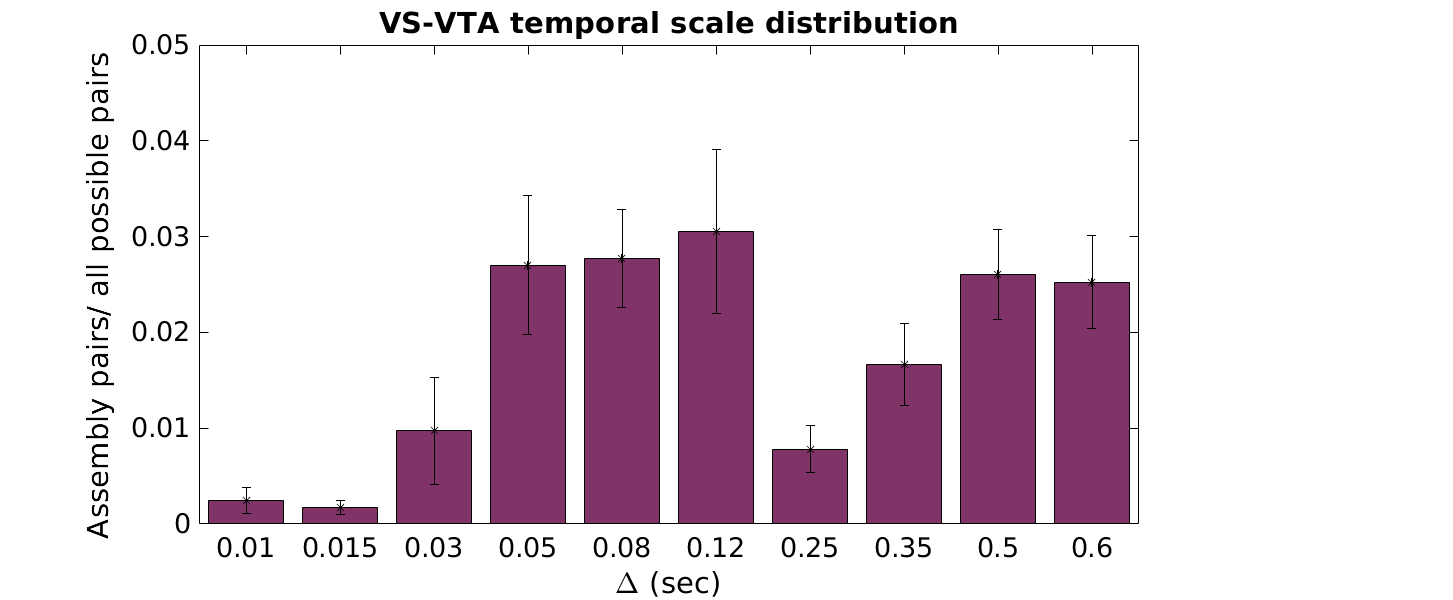
\includegraphics[scale=0.5]{figures/VS_VTA_Short1.png}
\caption{Bin distribution for inter-regional pairs. VS-VTA pairs show a bimodal distribution, revealing two temporal scale involved in inter-regional activation patterns.}
\label{fig:BinDistr}
\end{figure}
\begin{figure}[H]
%\centering
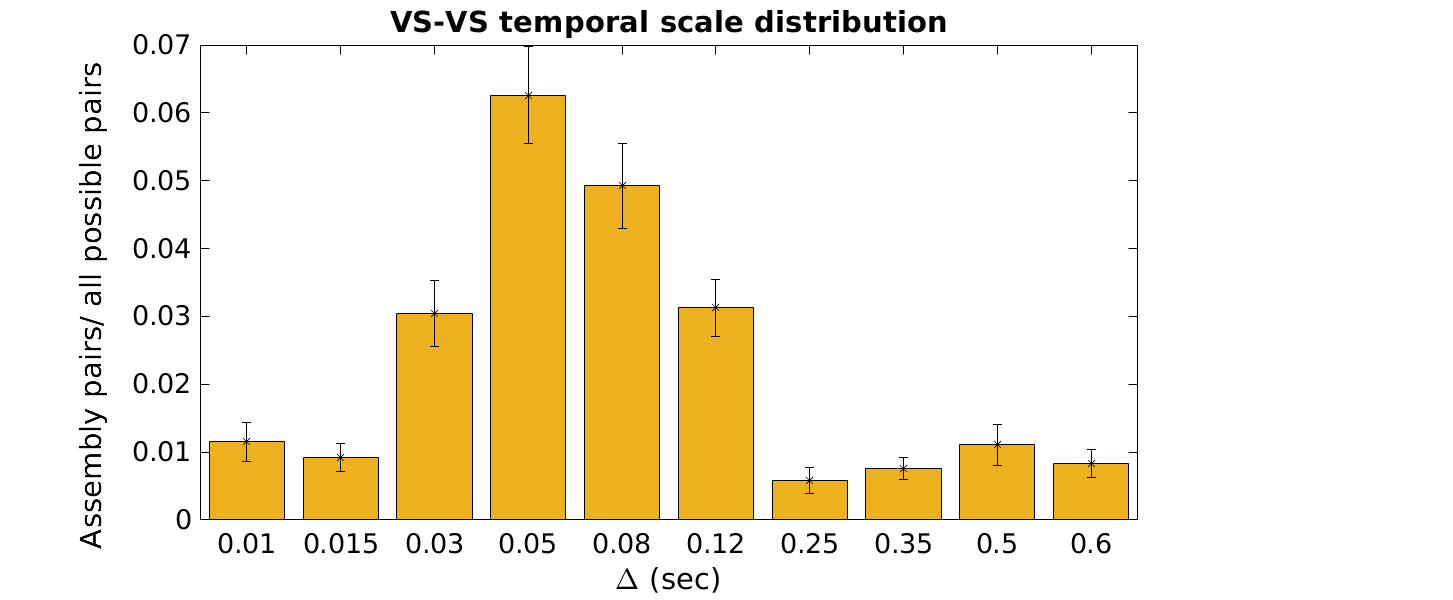
\includegraphics[scale=0.5]{figures/VS_VS_S.png}
\caption{VS-VS pairs are more precise than VS-VTA pairs and the bin distribution presents a peak at 50 $ms$}
\label{fig:BinDistrVS}
\end{figure}
\begin{figure}[H]
%\centering
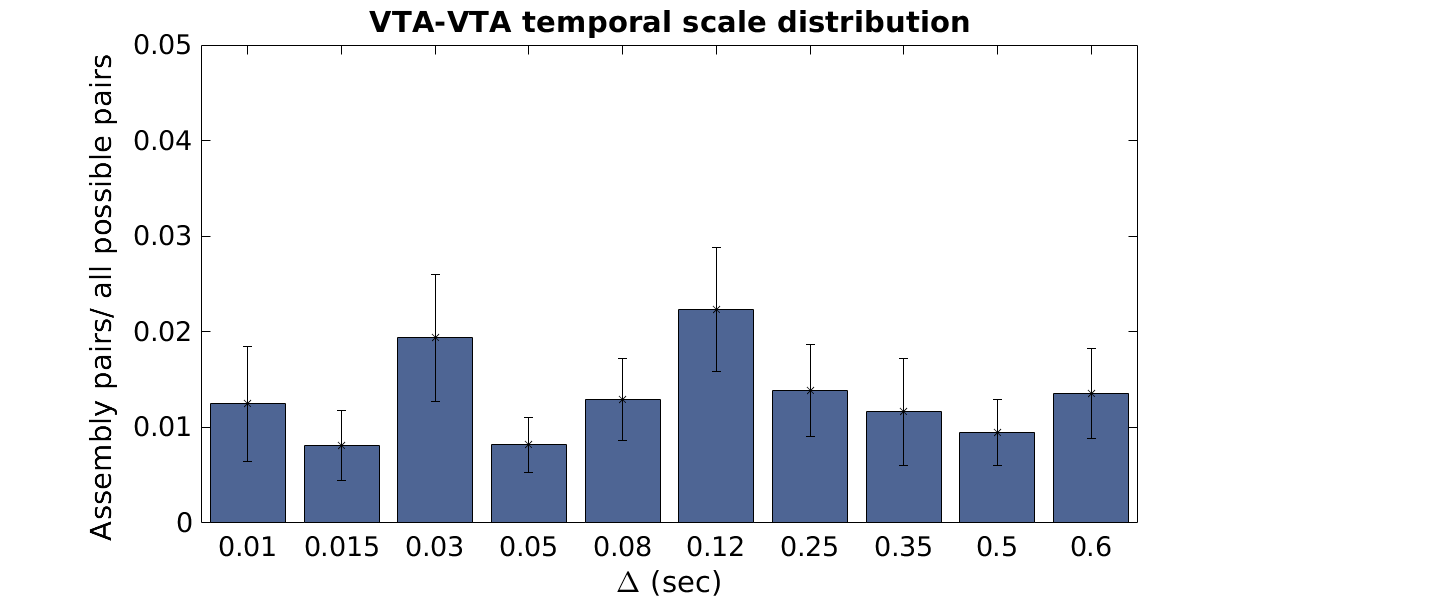
\includegraphics[scale=0.5]{figures/VTA_VTA_S.png}
\caption{VTA-VTA temporal scale distribution does not present any peak.}
\label{fig:BinDistrVTA}
\end{figure}
A comparison among inter-regional pairs (VS-VTA pairs) and intra-regional pairs (VS-VS pairs and VTA-VTA pairs) show interesting differences, that we are going to analyse.\\
While we observed assemblies of temporal precision at the scale of few tens of milliseconds only within either VS or VTA, assemblies of lower temporal precision were detected across VS-VTA units. Inter-regional VS-VTA interactions have a bimodal time-scales distribution with peaks around 80 $ms$ and one 1.6 $sec$, revealing two time scales involved in VS-VTA interaction, the first, more precise, ranged from 10 $ms$ to 250 $ms$, and the second including broader bin sizes; from which we consequently argue a complex interaction circuit effect, reflecting in inter-regional pairs.\\Bimodality is a characteristic specific of VS-VTA interactions, not present in VTA-VTA, or VS-VS interactions: intra-regional VTA-VTA pairs do not present any peak in time scales distribution, whereas intra-regional VS-VS bin size distribution is peaked around 50 $ms$.  
\subsection{SPN-FSN time scales interactions *}
\label{sec:SPN-FSN_Bin}
Fast spiking neurons population has broad firing rate, and according to the firing rate, sub-populations of the neurons classified as fast spiking neurons in first place can show different characteristic in terms of time-scales and length of interactions, or/and feature coding ({\color{red}ask for paper to cite}).\\From the distribution of mean firing rate of the recorded FSN was possible to define two sub-populations, those last do not present different characteristic when their units are coupled in assembly with a VTA neuron, however it worth to mention them in relation to their time-scales interactions with SPN. We report in figure \ref{fig:FSNsFireHisto} the histogram of FSNs mean firing rate, from which is possible to distinguish two sub-populations, that we will call FSNs low and FSNs high: the first characterized to have mean firing rate below $45 Hz$ and the latter has mean firing rate equal or above $45 Hz$.\\
\begin{figure}
    \centering
    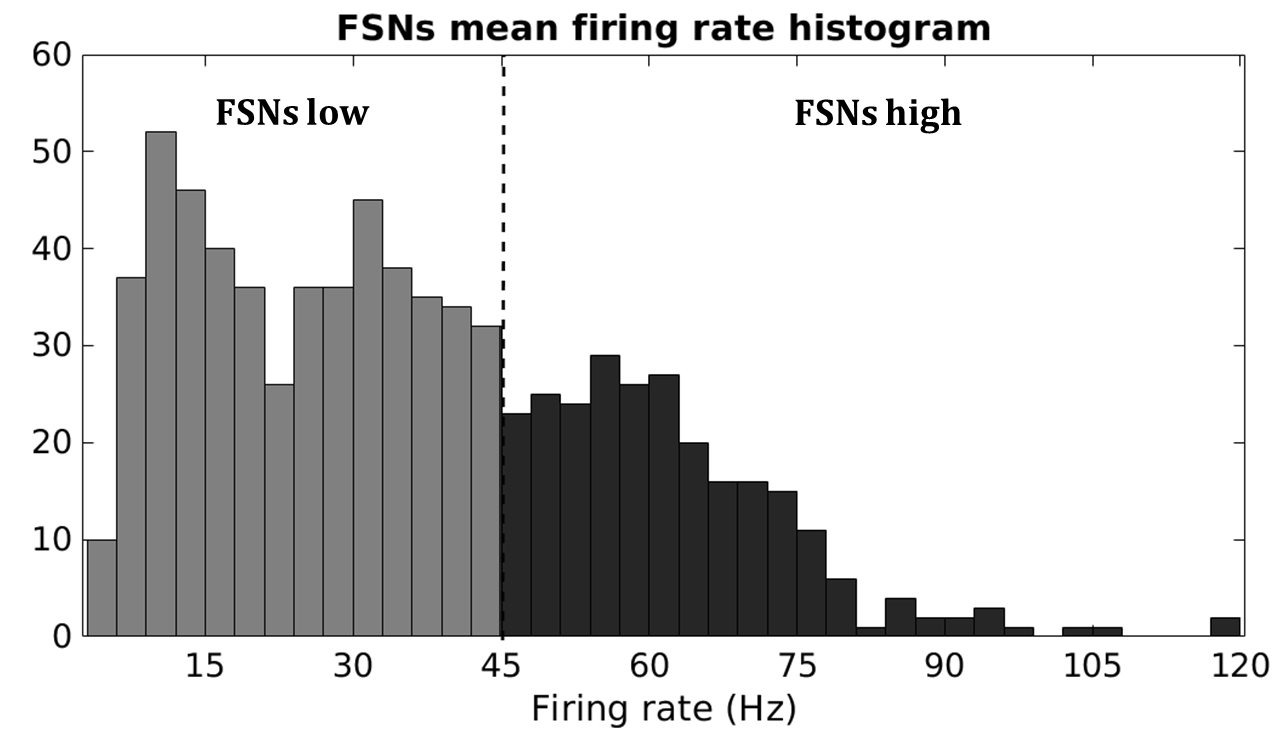
\includegraphics[scale=0.6]{figures/FSNFiringRateLightDark.pdf}
    \caption{Histogram of FSNs mean firing rate. We can distinguish two populations of FSNs: FSN low-firing-rate population (FSN-low), that are light grey in the graph, characterized by having a firing rate below 45 $Hz$, and FSN high-firing-rate population (FSN-high), in dark grey, characterized by having a firing rate from 45 $Hz$ upwards.}
    \label{fig:FSNsFireHisto}
\end{figure}
\begin{figure}
    \centering
    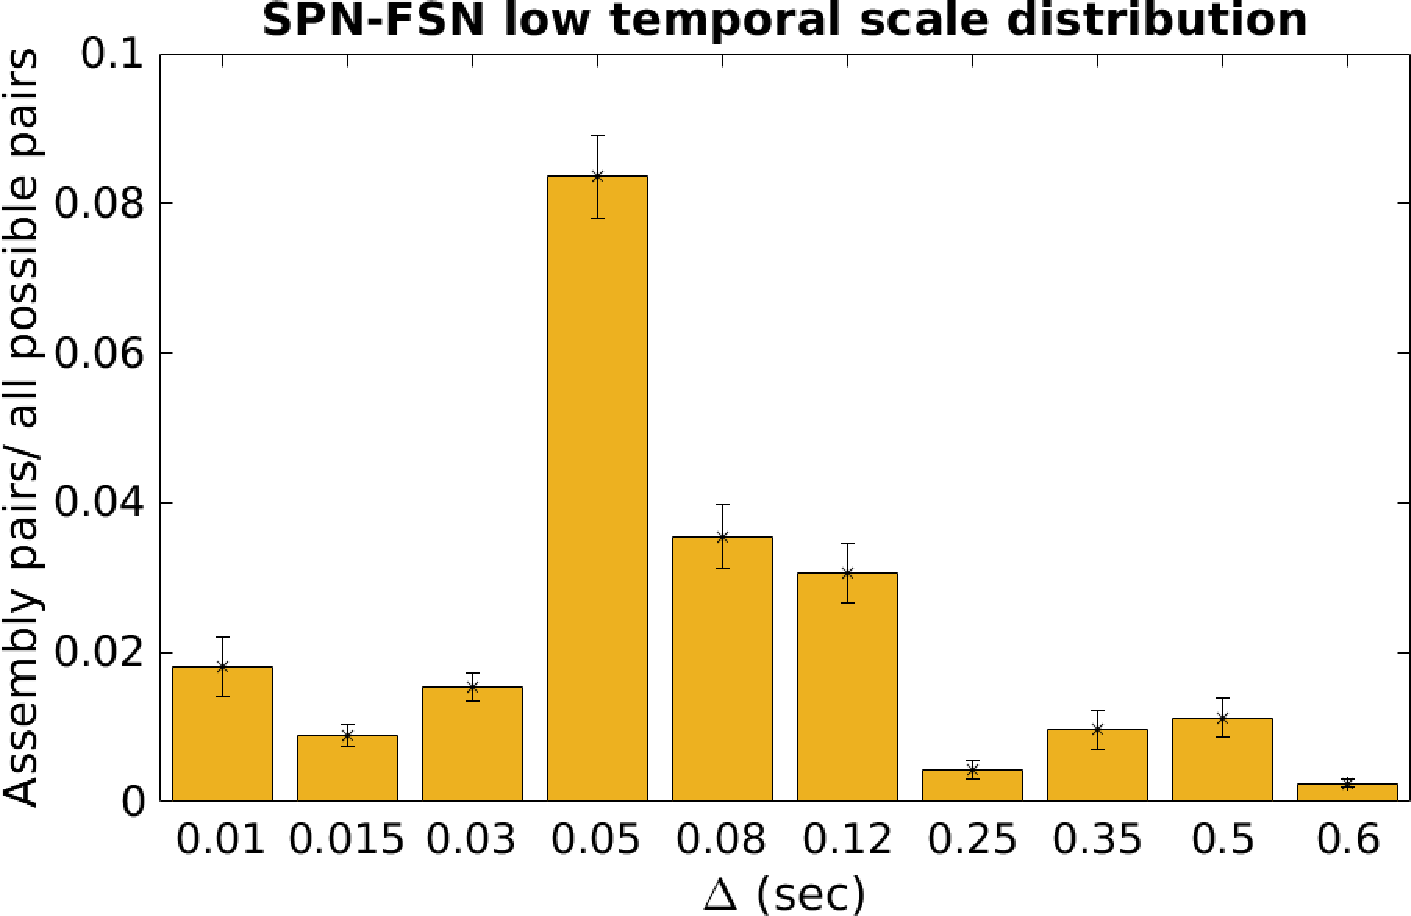
\includegraphics[scale=0.5]{figures/SPN_FSNlow1.pdf}
    \caption{SPN-FSN-low temporal scale distribution is peaked at 50 $ms$. A good portion of SPN-FSN-low pairs is detected also at 80 $ms$ and 120 $ms$.}
    \label{fig:SPN_FSNlowBin}
\end{figure}
\begin{figure}
    \centering
    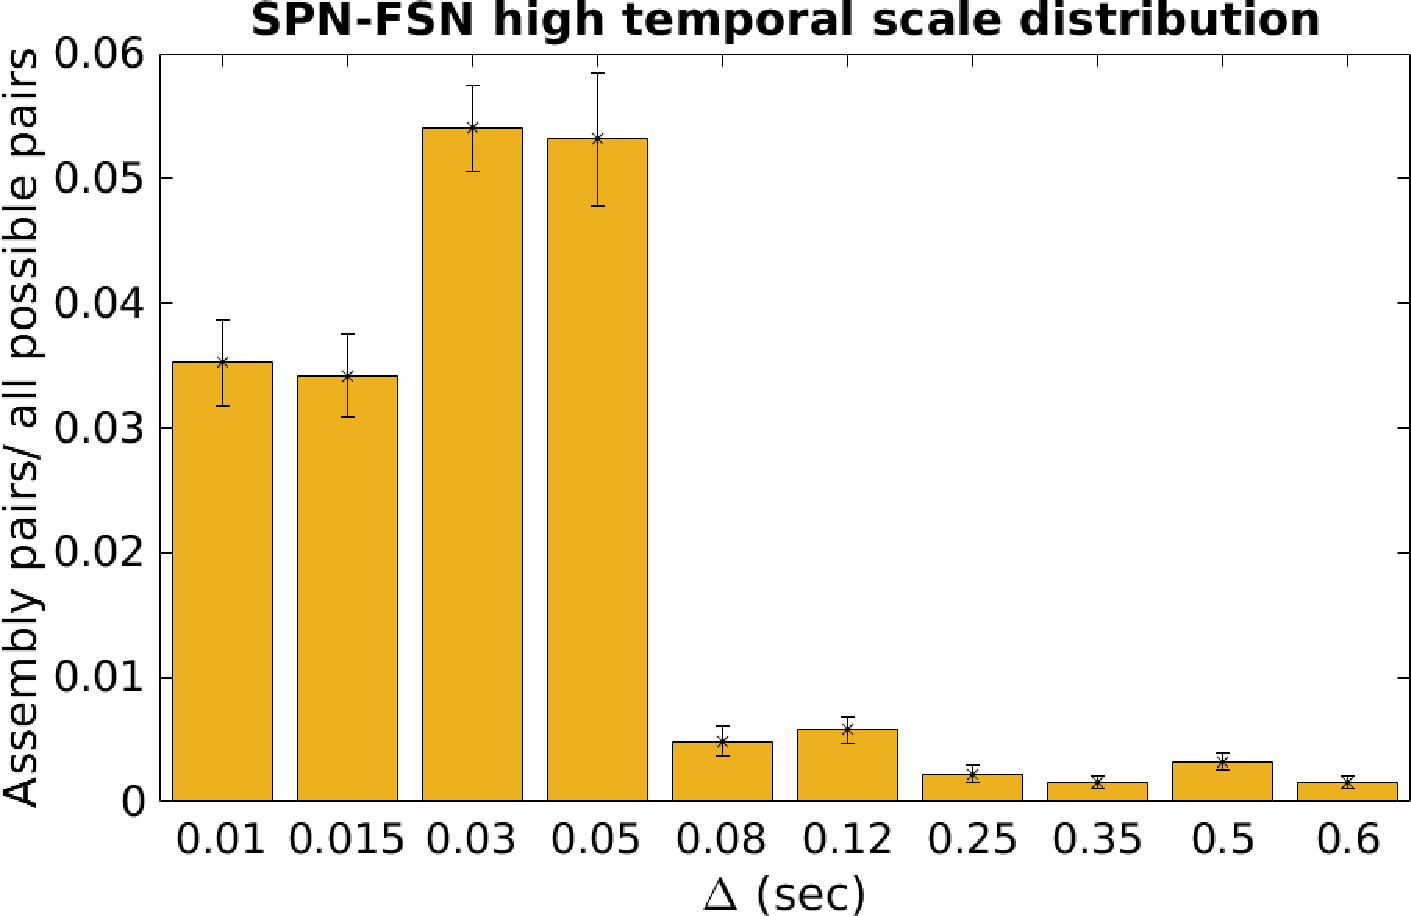
\includegraphics[scale=0.5]{figures/SPN_FSNhigh1.pdf}
    \caption{SPN-FSN-high pairs are almost exclusively detected at very precise time scales, namely from 10 $ms$ to 50 $ms$.}
    \label{fig:SPN_FSNhighBin}
\end{figure}
In VS we noticed differences between SPN-FSN-low pairs and SPN-FSN-high bin size distributions. SPN-FSN-low bin distribution pair is peaked at 50 $ms$, and another good portion of those pairs is detected at the two next bin sizes after the peak, 80 $ms$ and 120 $ms$ (fig. \ref{fig:SPN_FSNlowBin}); whereas SPN-FSN-high pairs are essentially only detected at more precise temporal scale (fig.\ref{fig:SPN_FSNhighBin}).\\We conclude that those two pair-types give a specific contribution to the global VS-VS temporal scale distribution. The variety of time scales involved in intra- or cross- area interactions in the studied regions emphasizes the complexity of the interaction circuit.
\section{Directionality} 
\label{sec:Directionality}
We had found in \hyperref[sec:TimeScales]{Section~\ref*{sec:TimeScales}} that inter-regional interactions have two characteristic time scales, which led us to consider more precise ($\Delta \in [0.01,0.25] ms$) and broader ($\Delta \in [0.25,0.6] ms$) VS-VTA pairs separately in the further study of directionality.\\We recall that one of the output of the cell-assembly algorithm is the inter-units activation lag of the assembly and, when we restrict the investigation to inter-regional pairs, the lag value tells us the distance in activation between the two region while the sign of the lag indicates the direction of the activation, namely which region became activated first and which one follows.\\
In fig.\ref{fig:LagInSecAll} we show the lag distribution for detected inter-regional pairs in the two characteristic time scales of interaction. As indicated in the plot, positive lag means VS is functionally leading the VTA activation and negative lag indicates the opposite direction.\\Interestingly lag distributions of precise and broad pairs are asymmetric, indicating that preferentially the VS activation leads the activation of the VTA. The two lag distributions show however remarkable differences: the lag distribution of broader pairs is fat-long tailed, that means a good portion of pairs detected with long activation lag ($lag > 1 sec$), whereas preciser pairs lag distribution has thin tails: almost all pairs detected in precise time scale have short lag ($|lag| < 1 sec$), and a good portion of pairs is detected within a lag value of 0.5 $sec$.\\
We focused the study on the more precise temporal scale, in such a way that temporal scale interactions were separated to typical task-related time scales, as e.g. the length of the odor duration, which cover typically an interval from 1.0 $sec$ to 1.5 $sec$.\\
We observed that, the directional assemblies are composed of striatal projection neurons leading dopaminergic neurons (SPN-DAN pairs), all the other pair-types do not show a clear preferred directionality. Furthermore, inter-unit activation lags of assemblies containing pallidal neurons (FSN) were shorter than those containing striatal projection neurons (SPN), compatibly with assumed connectivity. In fig.\ref{fig:LagInSec4typo} is shown the lag distribution for the four principal pair-types.\\
VTA dopaminergic neurons were laser tagged in first place, we can use the laser tagged units as control to validate the dopaminergic neurons classification; in fig.\ref{fig:LagInSecLaser} is shown the lag distribution of laser tagged dopaminergic units coupled with SPN and FSN. We can observe the similarity between the lag distribution of pairs containing laser tagged dopaminergic units and the lag distribution of the pairs containing classified dopaminergic units, in fact SPN-laser DAN pairs show directionality in direction $VS\rightarrow VTA$, whereas FSN-laser DAN are not directional, as we expected from the results obtained using classified units, which confirms the validity of the adopted classification.\\
\begin{figure}[H]
\centering
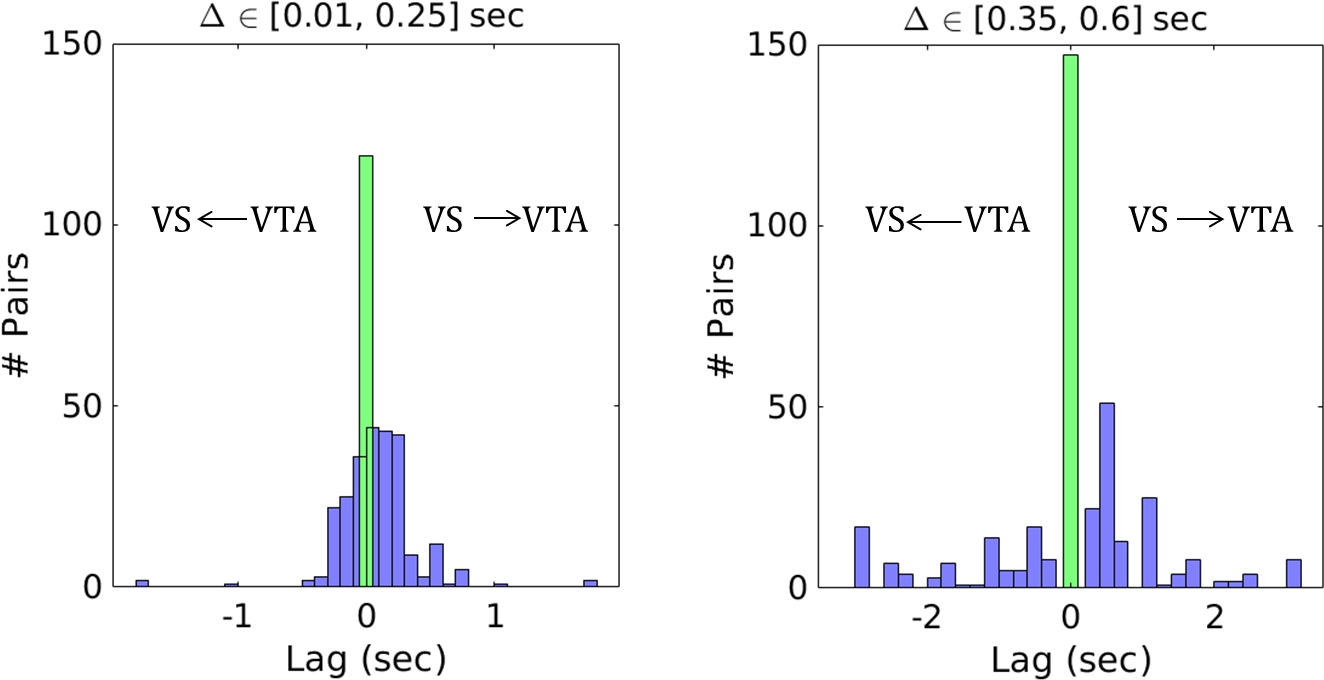
\includegraphics[scale=0.6]{figures/LagGeneral1.pdf}
\caption{Lag distribution for VS-VTA pairs in seconds. In green the synchronous pairs. On the left, lag distribution for pairs detected in more precise time scale. Slight distribution asymmetry indicates directionality in the direction of $lag > 0$, meaning a predominance of pairs in which VS leads VTA. On the right, the lag distribution for pairs detected in the broader time scale, it presented as an asymmetric fat-tailed distribution.}
\label{fig:LagInSecAll}
\end{figure}
\begin{figure}[H]
\centering
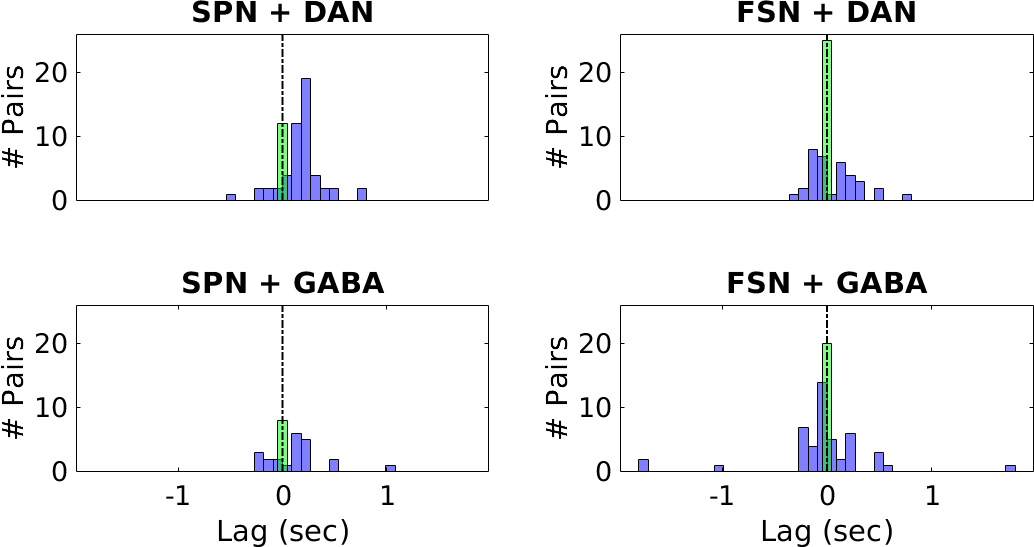
\includegraphics[scale=0.5]{figures/LagSec4Typo3VS.png}
\caption{Lag distribution of four more represented pair-types in precise time scale. Only SPN-DAN pairs show a preferred directionality, namely $VS\rightarrow VTA$.}
\label{fig:LagInSec4typo}
\end{figure}
\begin{figure}[H]
\centering
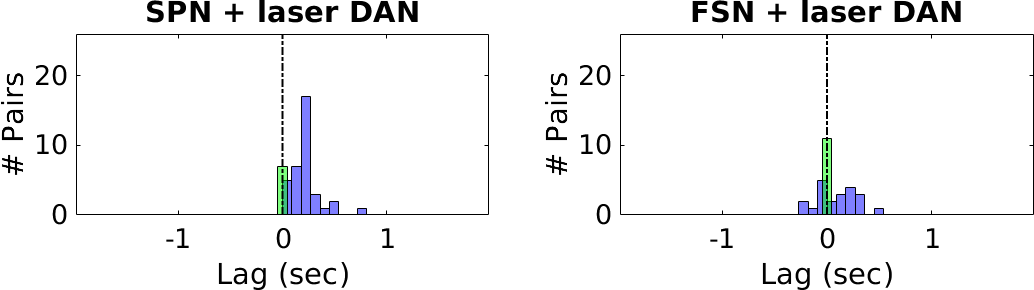
\includegraphics[scale=0.5]{figures/LagSecLaser3VS.png}
%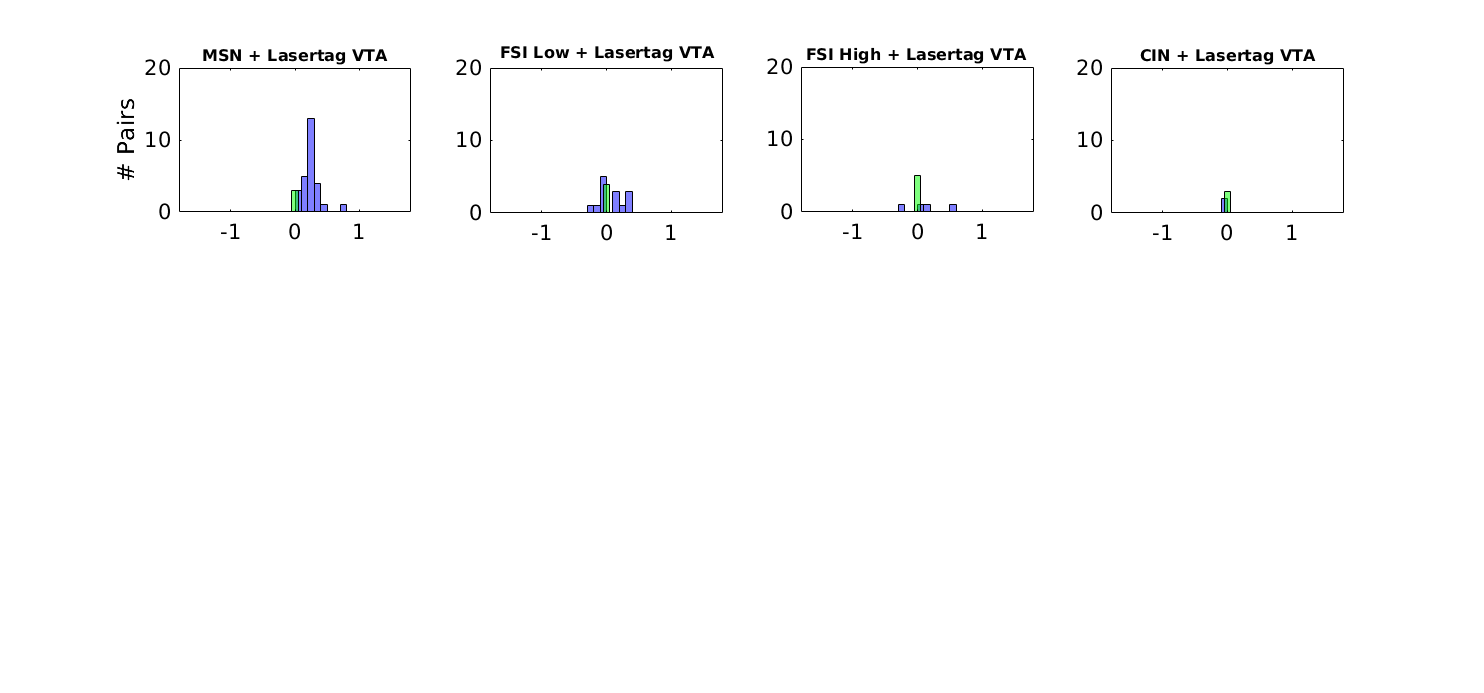
\includegraphics[scale=0.4]{figures/OnlyLaserOriz.png}
\caption{Lag distribution of laser tagged dopaminergic units in pair with SPN and FSN units, in precise time scale. Lag distributions are similar to the lag distributions of classified DAN in pair with SPN and FSN, confirming the directionality expressed by SPN-DAN pairs and the validity of the classification adopted in VTA.}
\label{fig:LagInSecLaser}
\end{figure}
The kind of activation exhibited by a directional pair is exemplified for an inter-regional directional pair in fig.\ref{fig:directional_assembly}. The pair in example was detected with a bin width of $\Delta = 0.12$, and the inter-units activation lag was positive with value 0.36 $sec$. On top is shown the mean across trials of the pair's activity for rewarded (grey line) and unrewarded odor (purple line) in the original phase, from the difference between the two activation lines, we say the illustrated pair specifically code for rewarded odor. On bottom are shown raster plot and mean firing rate of units in assembly. x-axis origin corresponds to the odour onset, while the red line marks the end of the stimulus duration.
Looking at the activity of two neurons, the directionality exemplified by the pair is evident, in fact we see first the VS unit becoming active and, after a temporal delay, the activation of VTA unit following. Raster plots show the stability of the activity across trials.\\ 
\begin{figure}
    \centering
    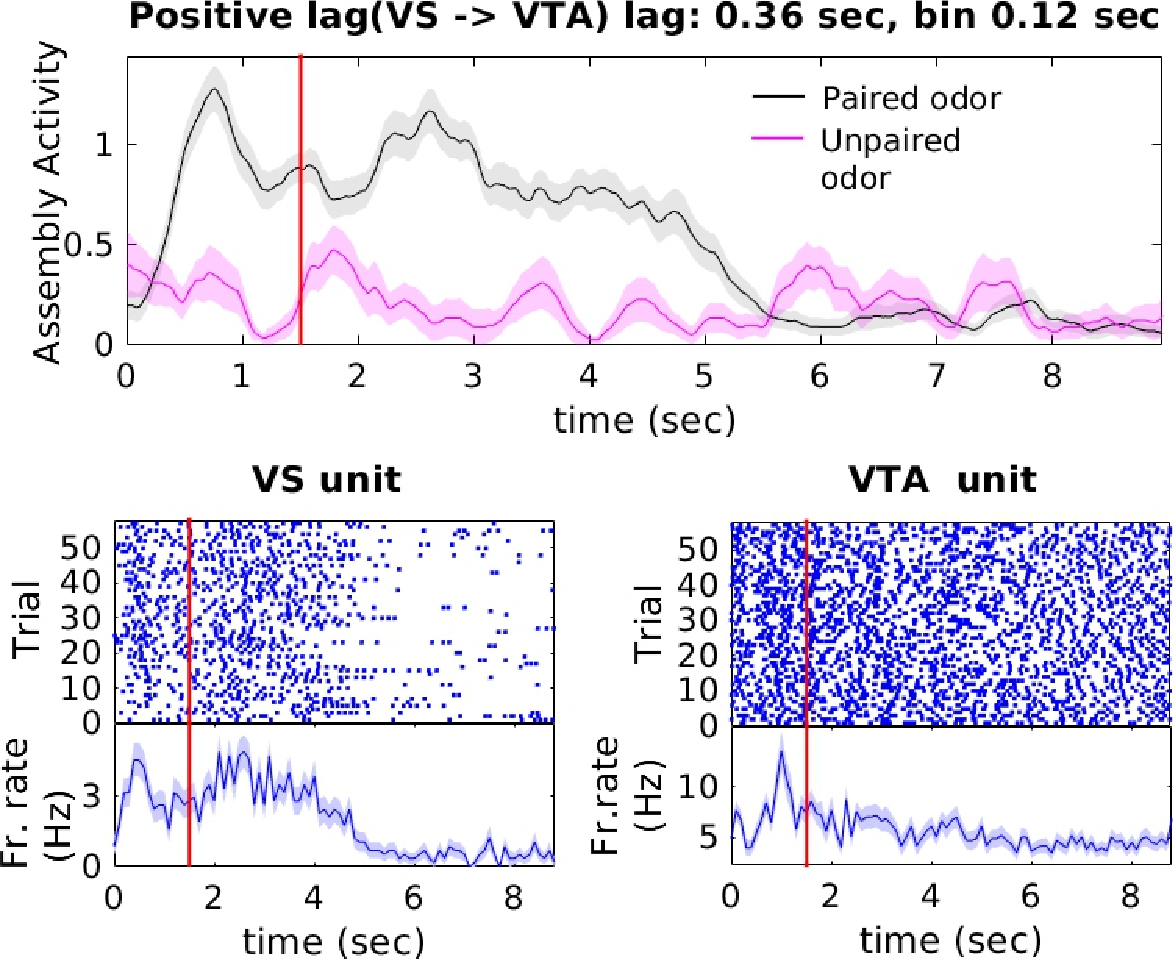
\includegraphics[scale=0.5]{figures/DirectionalAsEx1.pdf}
    \caption{Directional assembly. On top mean across trails and standard error of the activity of the pair for rewarded (grey) and unrewarded odour (purple) in the original phase. On bottom raster plot and firing rate (mean and standard deviation) of units in assembly. x-axis origin corresponds to the odor onset, while the red line marks the end of the stimulus duration. The examined assembly has a positive lag, that means VS preceding in activity VTA, from neuronal activity we can see in fact the VS unit activate before than the VTA unit.}
    \label{fig:directional_assembly}
\end{figure}
At the end of the temporal scales and directionality investigation, we make the hypothesis that the time scale segregation reveals different assembly-activation patterns, as one can see from an example of activation pattern segregation in fig.\ref{fig:AsActBinLag}, where we show the heat map of inter-regional pairs activity averaged across trials in one of the paradigms of the experiment.\\Pairs exhibiting directionality $VS \rightarrow VTA$ and detected in the precise time scale ($\Delta \le 0.25$) became activated early during the odour presentation, a good portion of them show a second activation after the odour presentation.\\The early activation at the stimulus presentation is the type of activation we expect when the animal predicts the reward, as discussed in \hyperref[sec:StateArt]{Section~\ref*{sec:StateArt}}, moreover we have shown in fig.\ref{fig:LagInSec4typo} as the SPN-DAN pairs are directional, thus we speculate that SPN-DAN are good candidate for reward prediction (RP) coding; the investigation of this hypothesis will be argument of the next chapters.\\
\begin{figure}
    \centering
    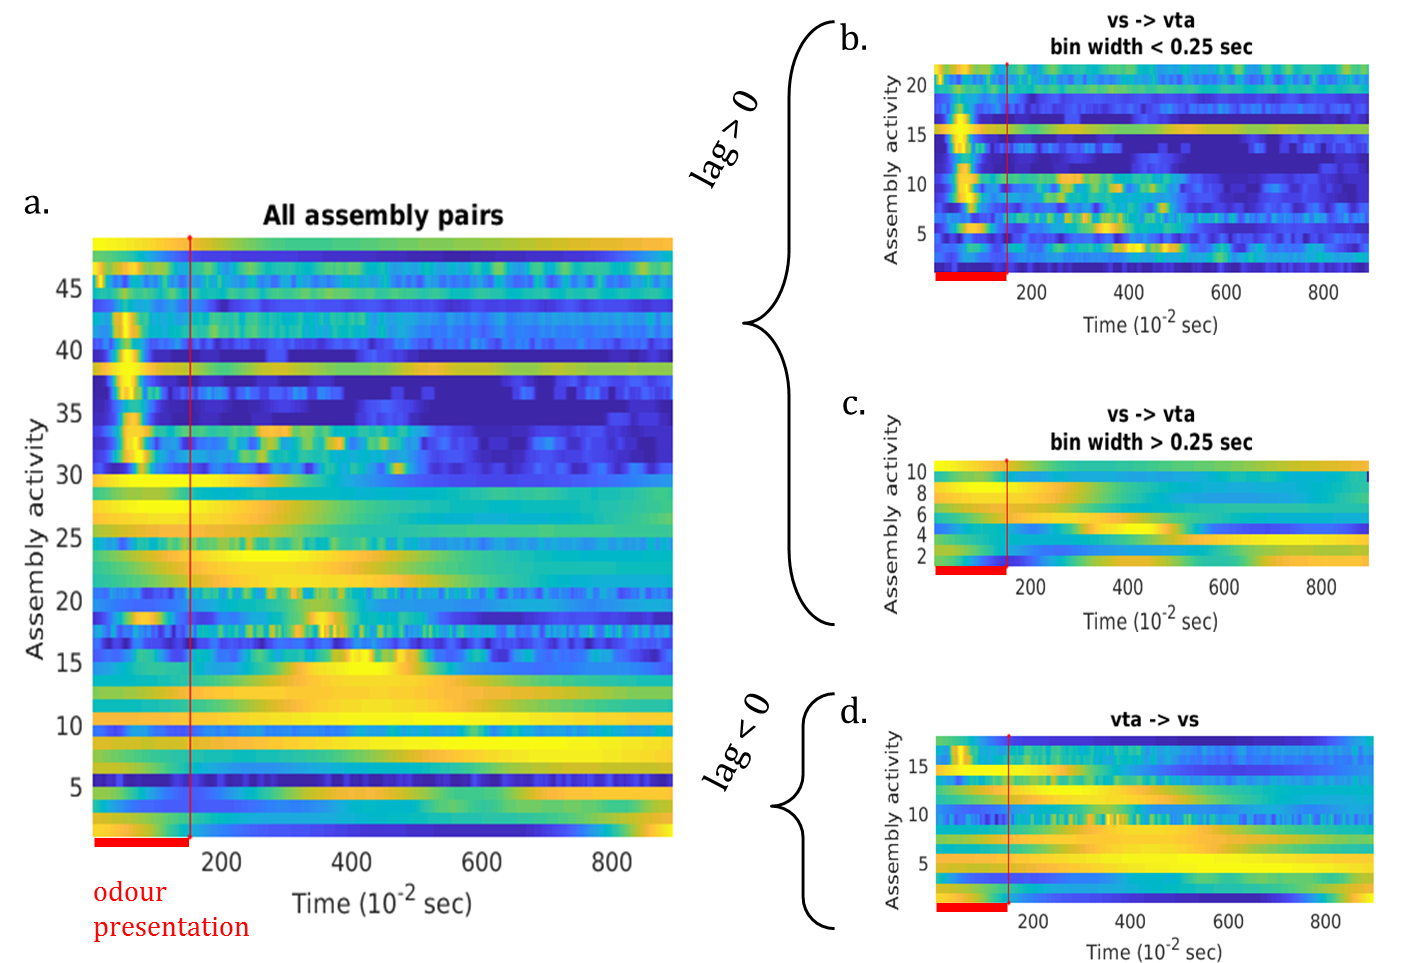
\includegraphics[scale=0.45]{figures/AsActPerBinLag1.png}
    \caption{Assembly-activation patterns given time bins and lags. In a.) heat map of inter-regional pairs in one the experimental paradigms, b,c,d. pairs of a. selected for bin size ($\Delta$) and lag: $\Delta < 0.25 s$ and $lag > 0$ (b.), $\Delta > 0.25 s$ and $lag > 0$ (c.), $lag < 0$ (d.)}
    \label{fig:AsActBinLag}
\end{figure}
\section{Conclusion}
From the inter-regional time scales distribution we deduced VS-VTA pairs have two time scales of interaction, which highlights the complexity of VS-VTA pair interactions and underlines the importance to choose a method capable to explore different time scales.\\The two time scales involved in VS-VTA interaction were then separated to continue the study with the lag analysis, from which emerged a preferred directionality in the verse $VS\rightarrow VTA$ in pairs containing striatal projection neurons and dopamaninergic neurons.\\The study of bin widths and lags of pairs depicted differences among different time scales of interaction and directionalities. We assume a segregation in activation patterns derived from time scales and directionality segregation; in that direction, as preliminary investigation, we have shown in a small portion of the data-set that, pairs detected at the precise time scale and exhibiting the directionality $VS\rightarrow VTA$ show an activity pattern in agreement with the reward prediction coding.\\Since directional assemblies are formed by striatal projection neurons and dopaminergic neurons, we hypothesize that those pairs are good candidate for prediction error coding. This question will be the \textit{fil rouge} of the next chapter, in other words we ask whether different pair-types have different coding feature. The starting point of the analysis is the pair-types task related response. A systematic analysis of this is performed in \hyperref[sec:TaskResp]{Section~\ref*{sec:TaskResp}}.

 \section{Pair-types task-related pattern}
 \label{sec:TaskResp}
 In the previous section we conclude that time scale segregation and directionality might reflect specific task-related coding feature, using an example we have shown how different directionality reveal different pairs activity patterns. We have seen as well that different assembly-pairs have different directionality distribution and SPN-DAN assembly-pairs, in particular, exhibit a clear $VS\rightarrow VTA$ directionality.\\Thus we investigate in this section if different assembly-pairs-types have different task-related activity patterns, which express different task-related feature coding.\\
 Thus we analysed the assembly-pairs activity during the relevant task moments, namely the stimulus presentation, the moment preceding the reward, and the reward retrieval.\\We tested the responsiveness of each assembly-pair in specific time intervals through a paired Friedman's test. The chosen time intervals were 0.5 $sec$ long.
 In fig.\ref{fig:HeatPairsDan} assembly-pairs tested with Friedman's test and resulting to have significant task related response in original phase. In order: A1. SPN-DAN assembly-pairs in original phase: a good portion of those pairs became active early at the rewarded stimulus (CS+) presentation, a good portion remains active during the stimulus presentation (CS+ cont.), until the reward retrival (US), only a small fraction is active only in US window, this kind of answer makes those assembly-pair-types good candidate for Reward Prediction (RP) coding. In A.2 the same assembly-pairs in the reversal phase. FSN-DAN assembly-pairs on contrast have a phasic response to the rewarded stimulus (CS+) and reward retrival (US) (B.1); in B.2 same FSN-DAN pairs in the reversal phase, a good portion of units responsive to CS+ in original phase, became in reversal responsive to US. This kind of answer makes those assembly-pair-types good candidate for Reward Prediction Error (RPE) coding.
 \begin{figure}
     \centering
     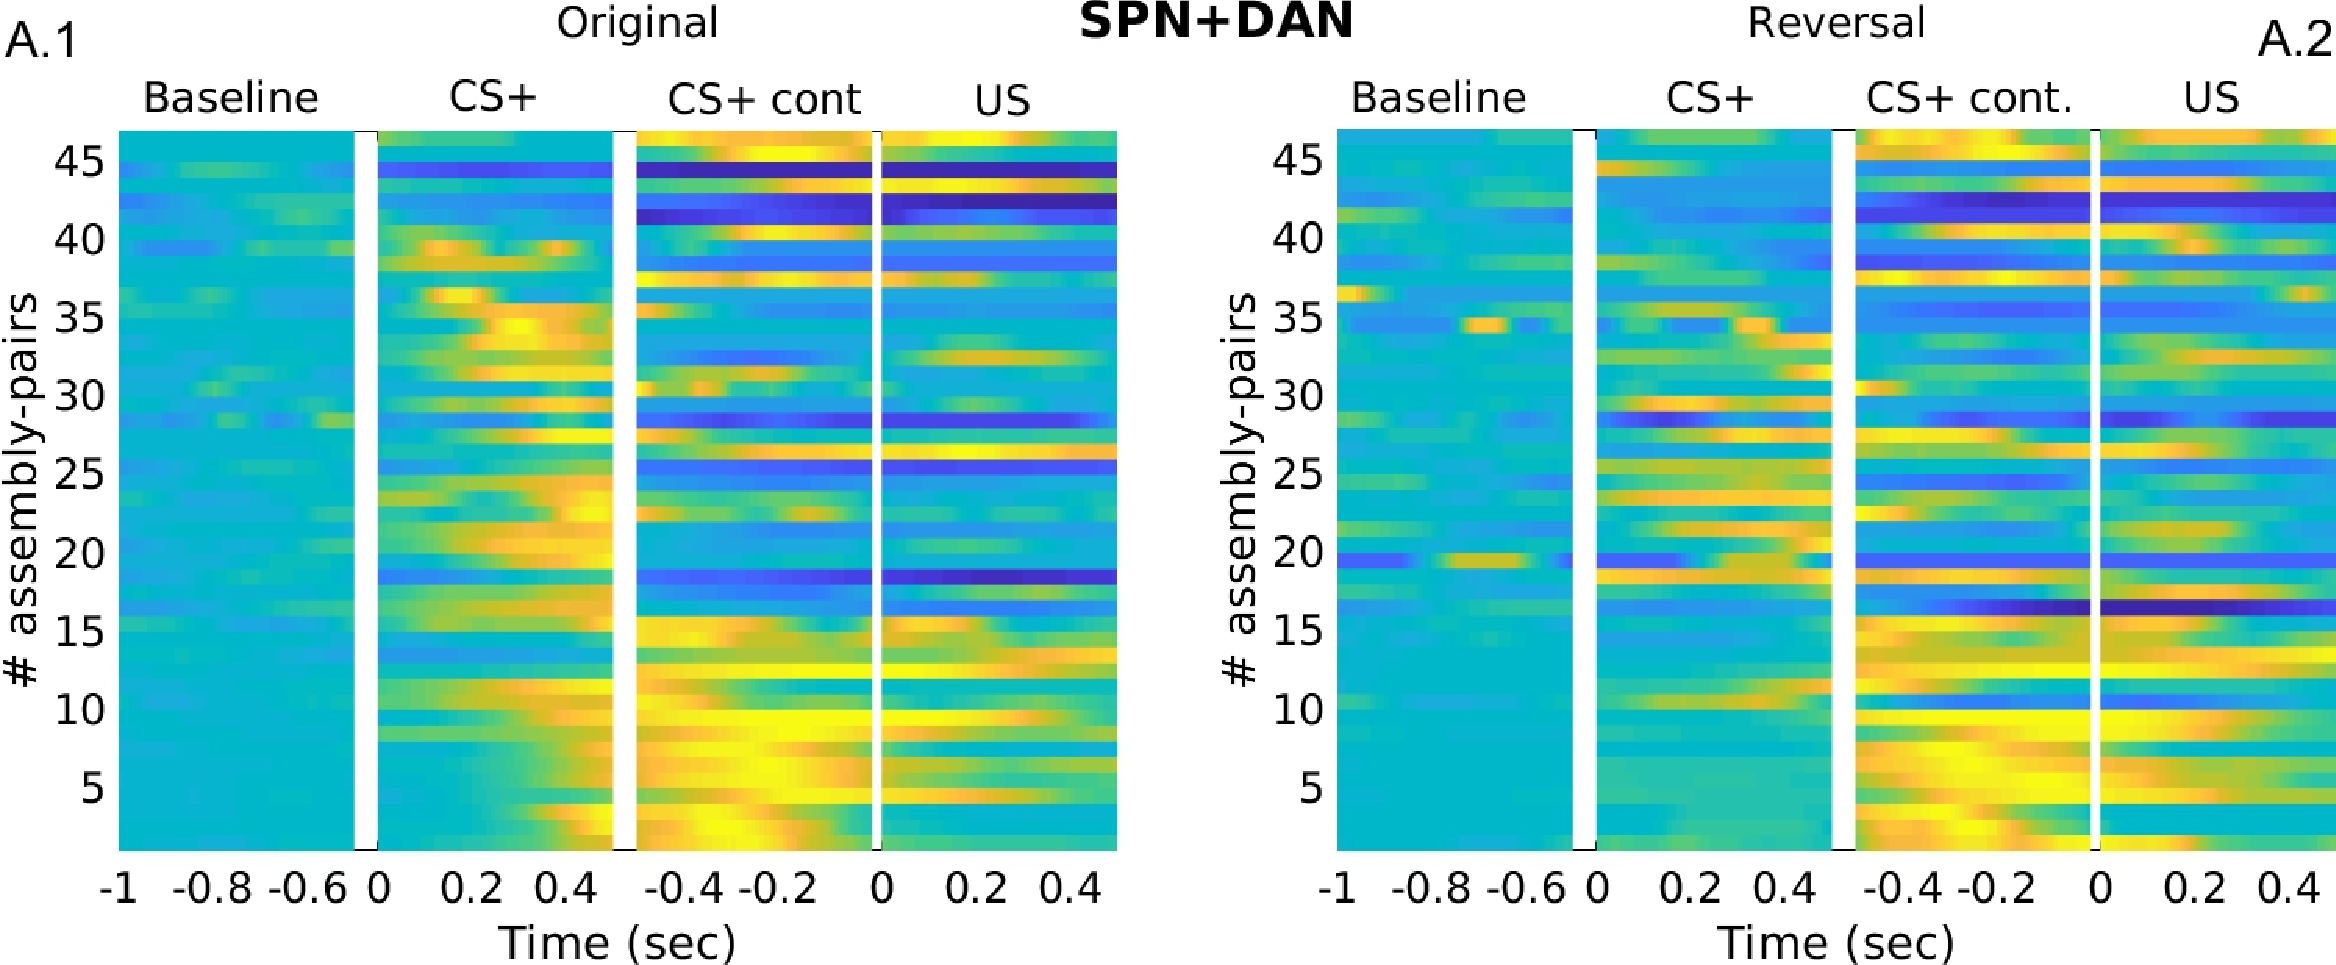
\includegraphics[scale=0.36]{figures/HeatSPN_DAN.pdf}
     
     \vspace{1cm}
     
     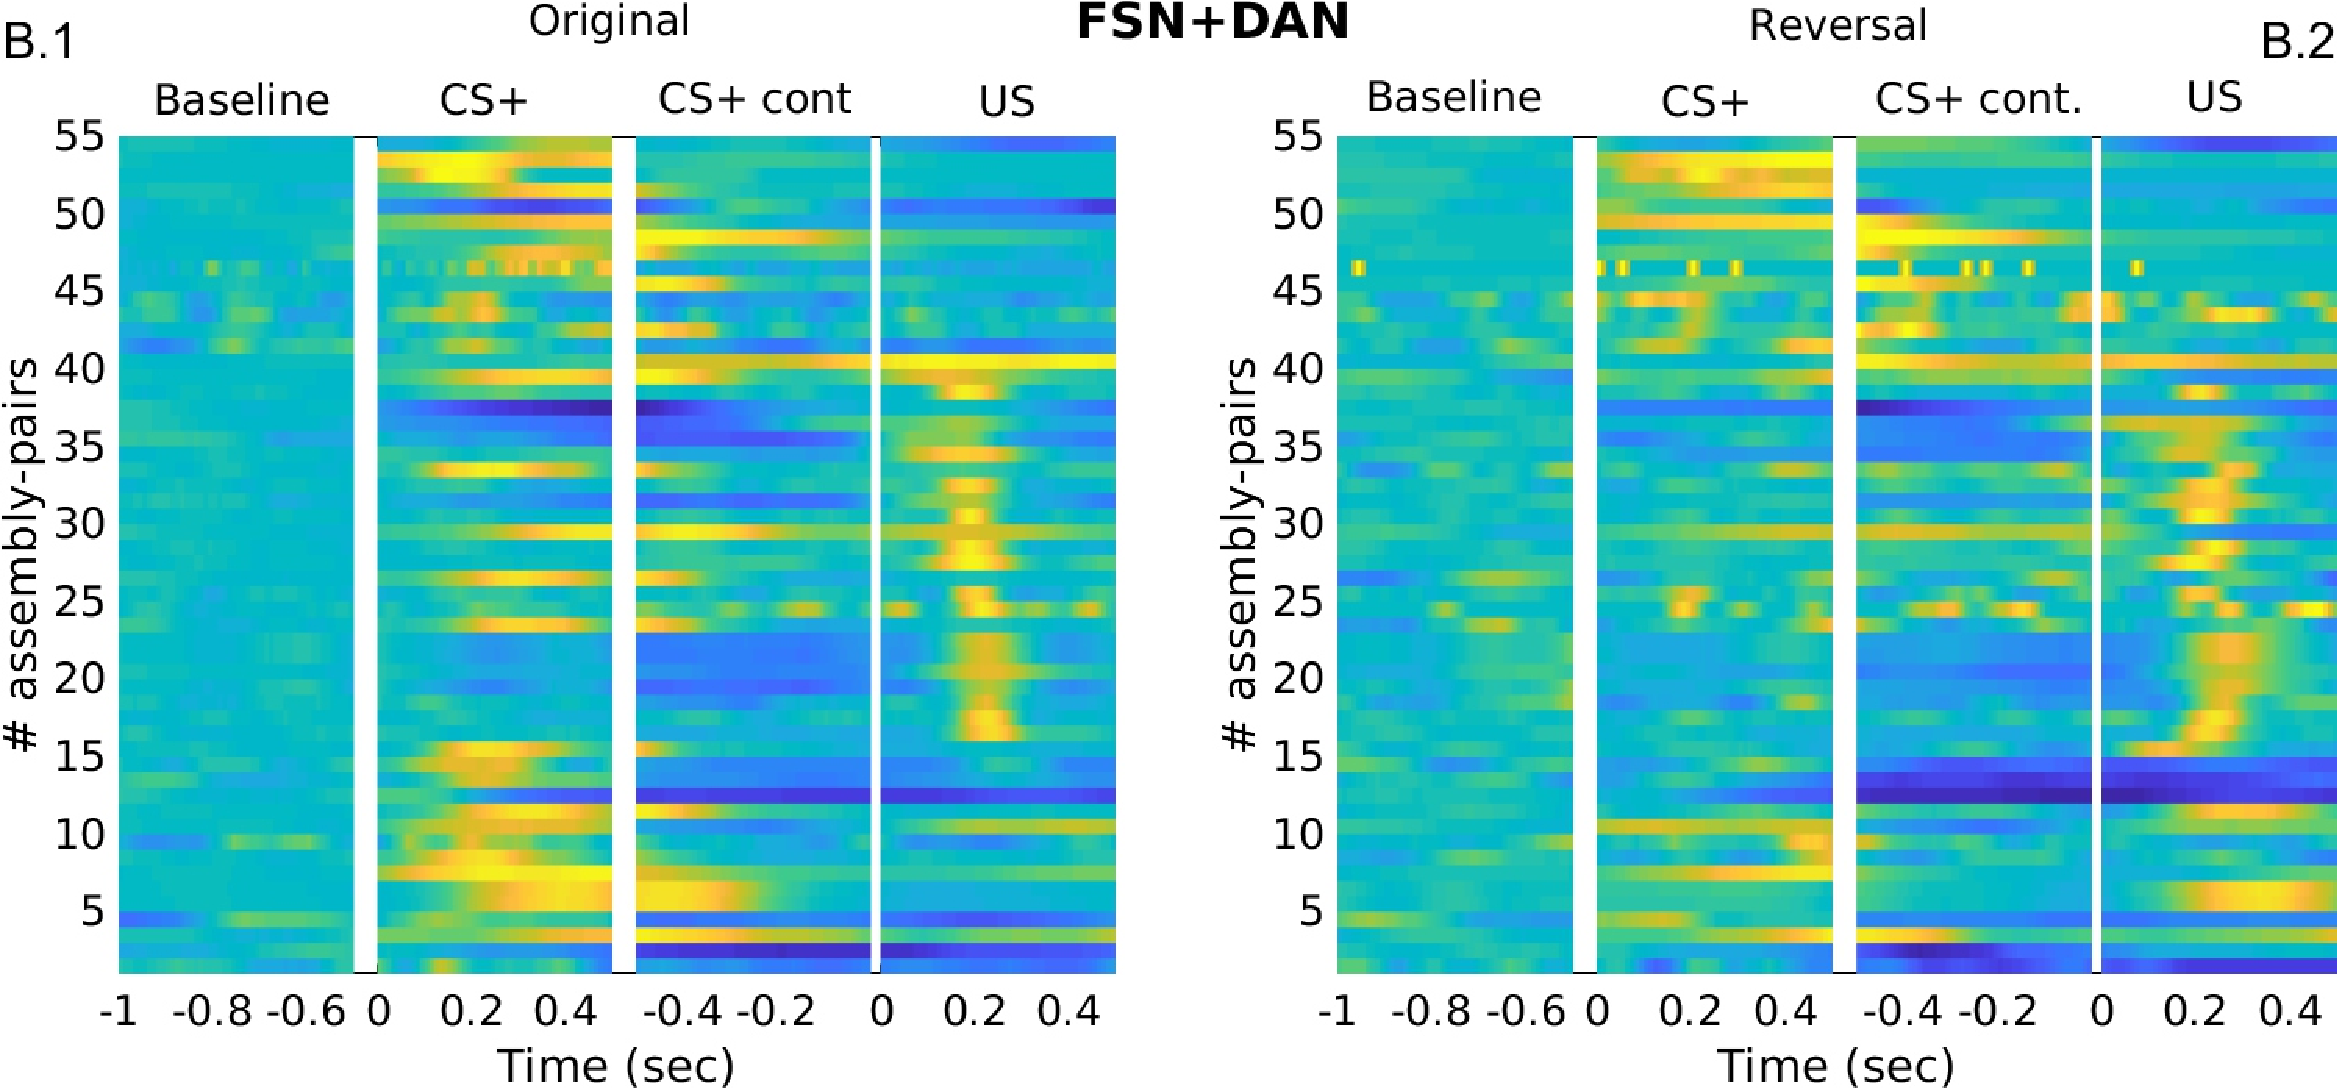
\includegraphics[scale=0.36]{figures/HeatFSN_DAN.pdf}
     \caption{Assembly-pairs tested with Friedman's test and resulting to have significant task related response in original phase. In order: A1. SPN-DAN assembly-pairs in original phase: a good portion of those pairs became active early at the rewarded stimulus (CS+) presentation, a good portion remains active during the stimulus presentation (CS+ cont.), until the reward retrieval (US), only a small fraction is active only in US window, this kind of answer makes those assembly-pair-types good candidate for Reward Prediction (RP) coding. In A.2 the same assembly-pairs in the reversal phase. FSN-DAN assembly-pairs on contrast have a phasic response to the rewarded stimulus (CS+) and reward retrieval (US) (B.1); in B.2 same FSN-DAN pairs in the reversal phase, a good portion of units responsive to CS+ in original phase, became in reversal responsive to US. This kind of answer makes those assembly-pair-types good candidate for Reward Prediction Error (RPE) coding.}
     \label{fig:HeatPairsDan}
 \end{figure}
 \begin{figure}
     \centering
     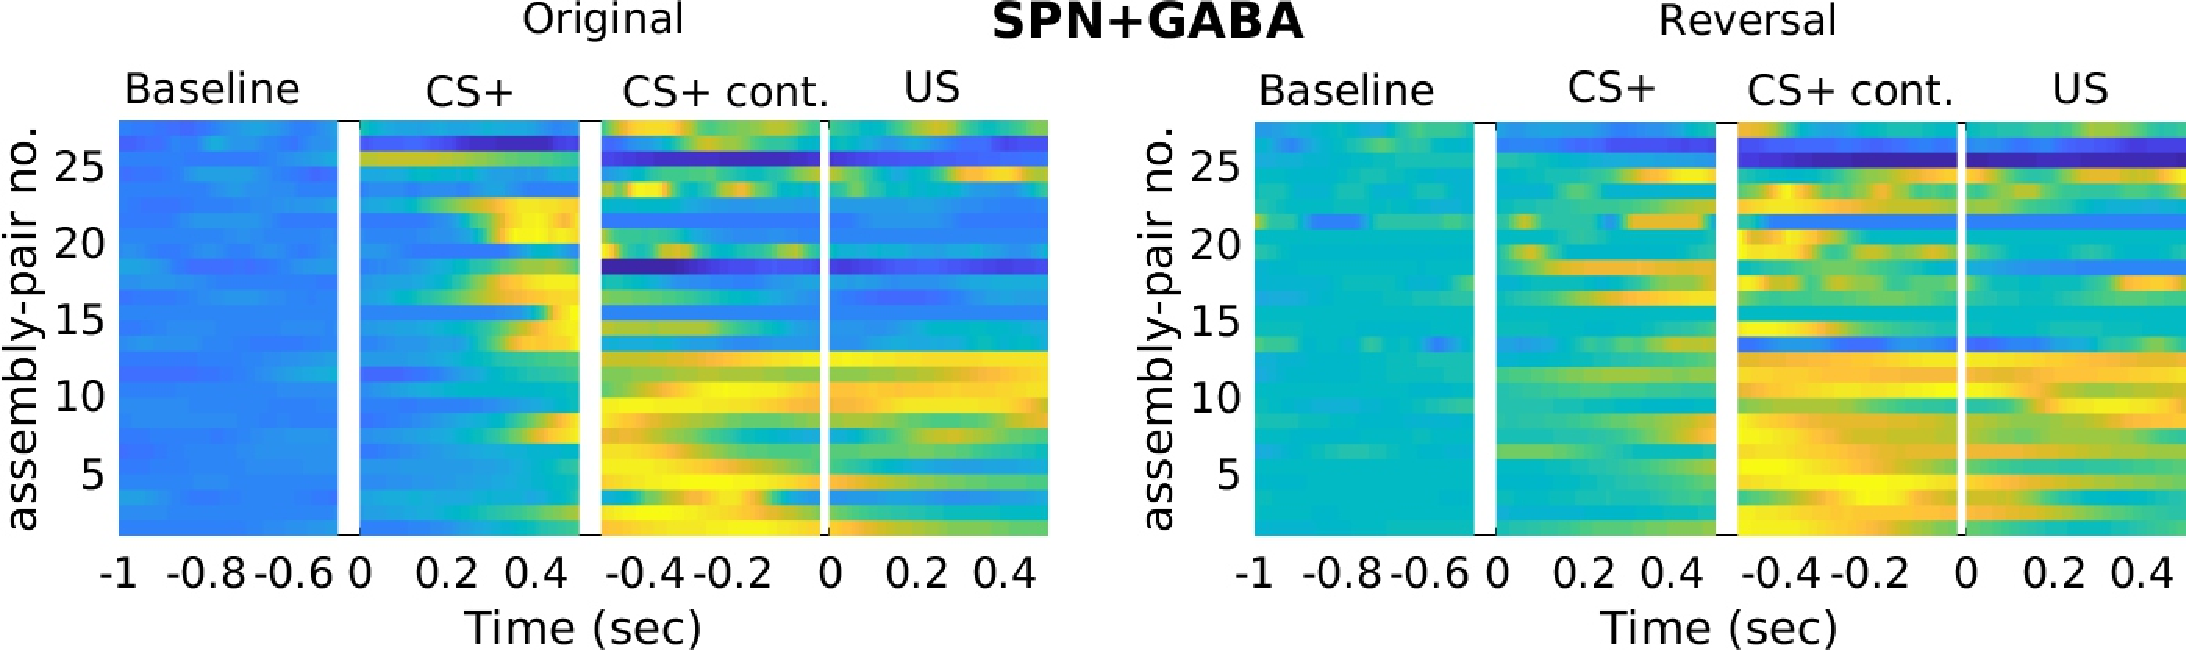
\includegraphics[scale=0.36]{figures/HeatSPN_GABA.pdf}
     
     \vspace{1cm}
     
     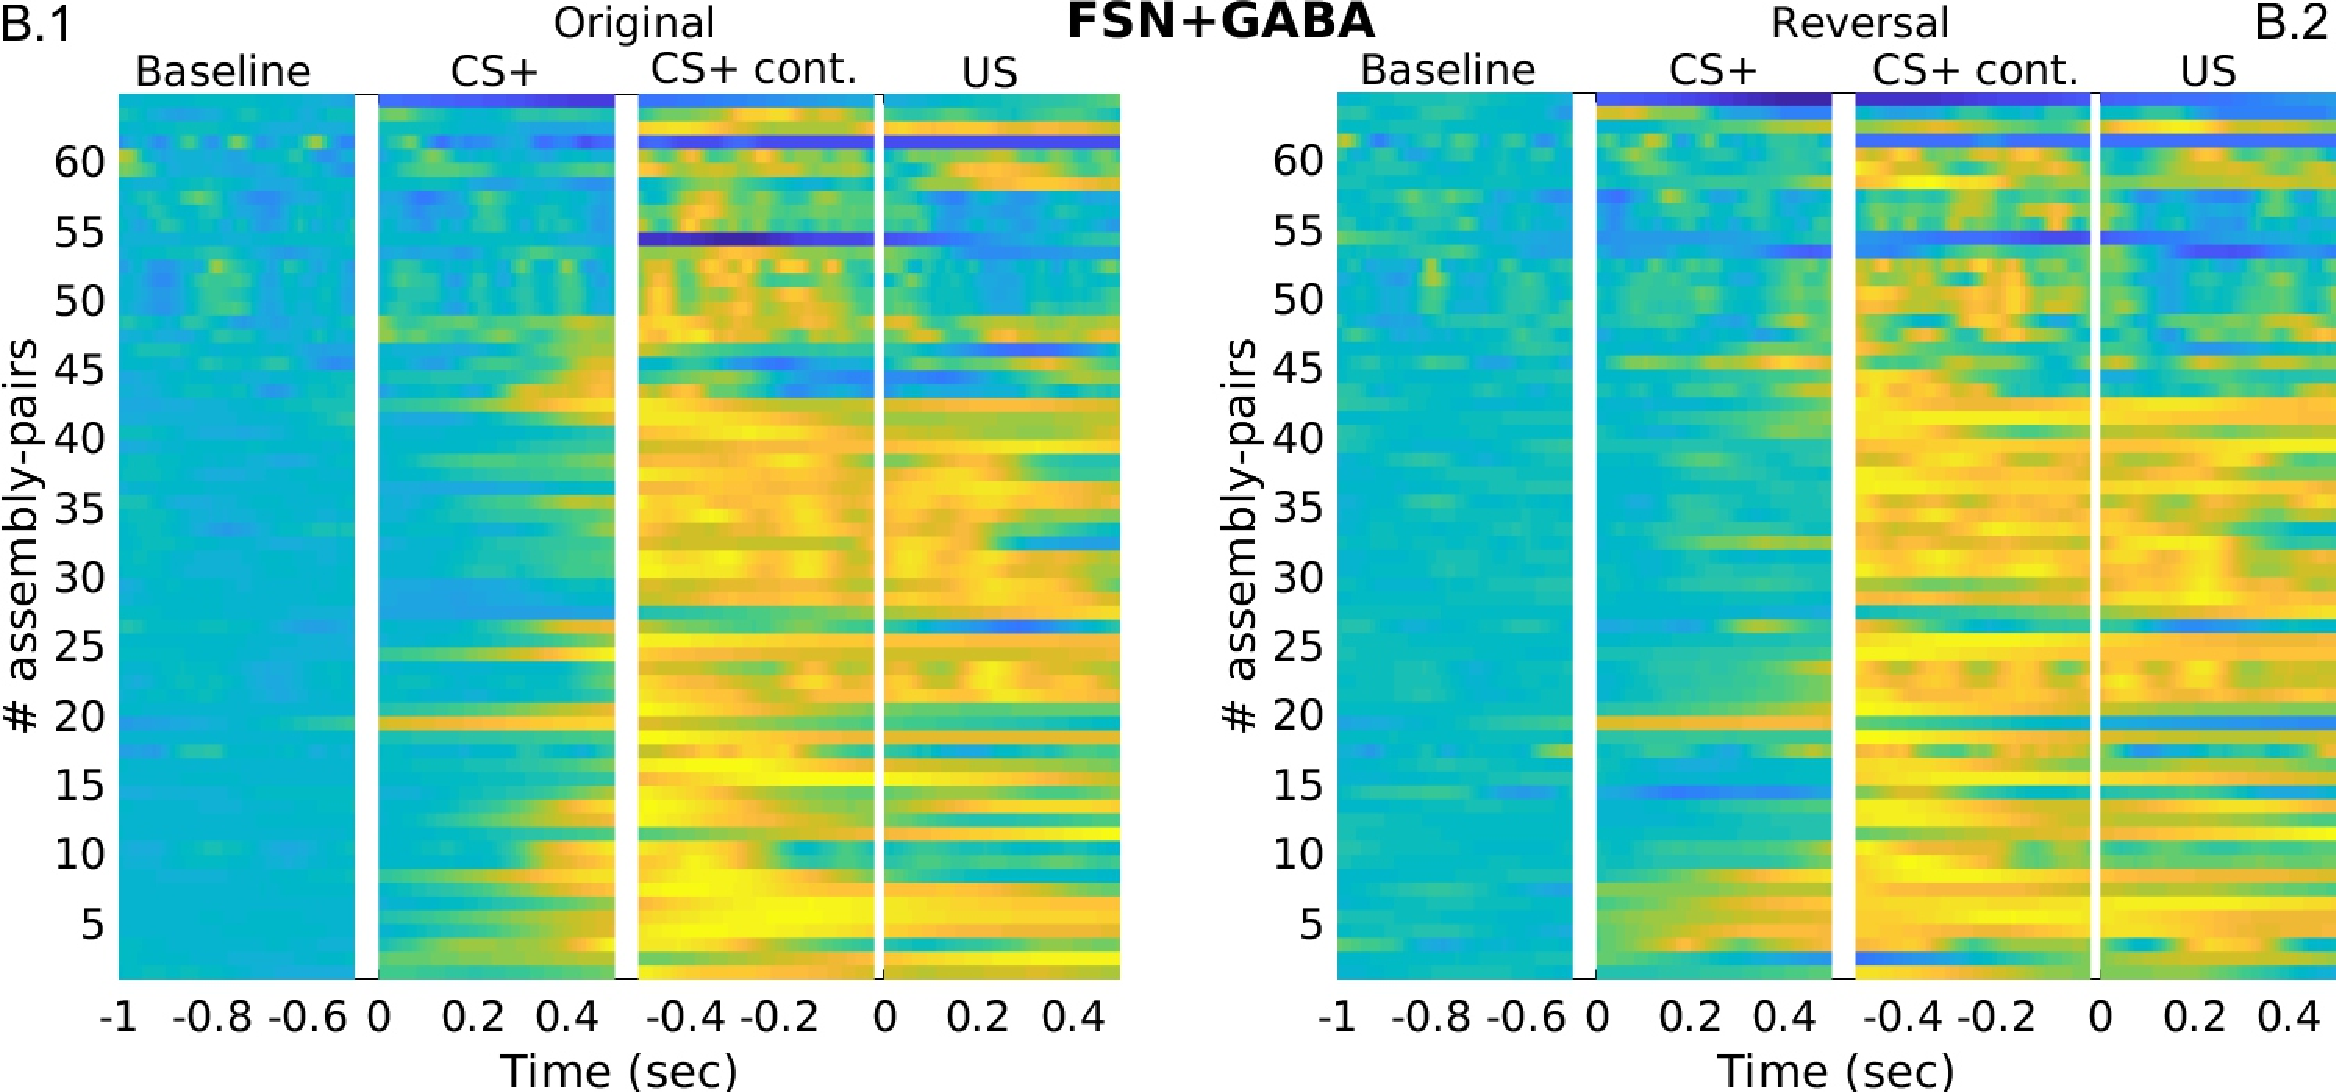
\includegraphics[scale=0.36]{figures/HeatFSN_GABA.pdf}
     \caption{Assembly-pairs tested with Friedman's test and resulting to have significant task related response in original phase. In order: in A.1 SPN-GABA assembly-pairs in original phase: a good portion of those pairs became active during the rewarded stimulus presentation (second half of CS+ and CS+ cont.), a good portion shows tonic activity until the reward retrieval (US). In A.2 the same assembly-pairs in the reversal phase. In B.1 FSN-GABA assembly-pairs are tonically active from the second half of the rewarded stimulus presentation window (CS+) to the reward retrieval window.}
     \label{fig:HeatPairsGaba}
 \end{figure}
 %%%%%%%% Commento forse da buttare
 %First difference between original and reversal phase is number of assemblies responding during the post-stimulus interval, this number decrease for all the typologies involved during hit trials (as shown in fig. (\ref{fig:histo_taskrel})), in according to the intuition, in reversal phase in fact, when the animals became more expert, neuronal response tend to be shifted closer to the reward delivery. This effect can be seen in fig. (\ref{fig:NeusInAsse}) where activity and raster plots of two units in a pair are shown. Looking at the raster plots, a shift in correspondence to the phase-switch is evident in both units.
 %\begin{figure}
  %   \centering
  %   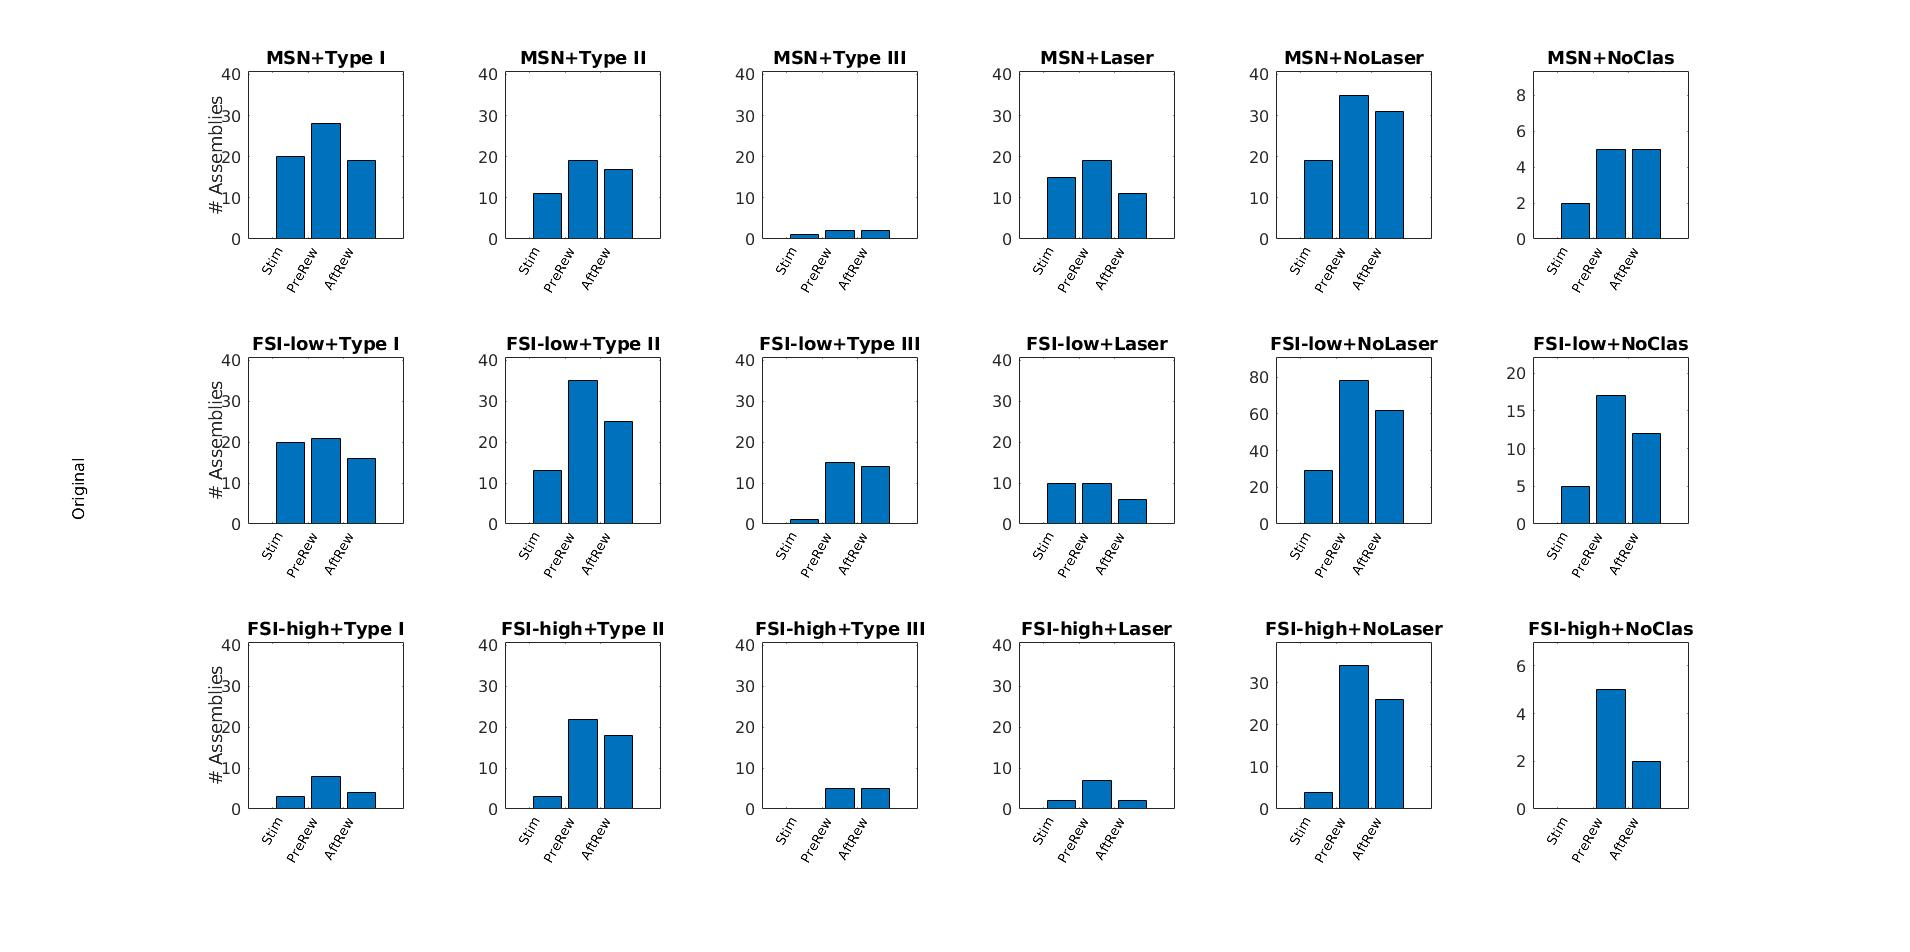
\includegraphics[scale=0.3]{figures/Original_Hit_N.jpg}
    % 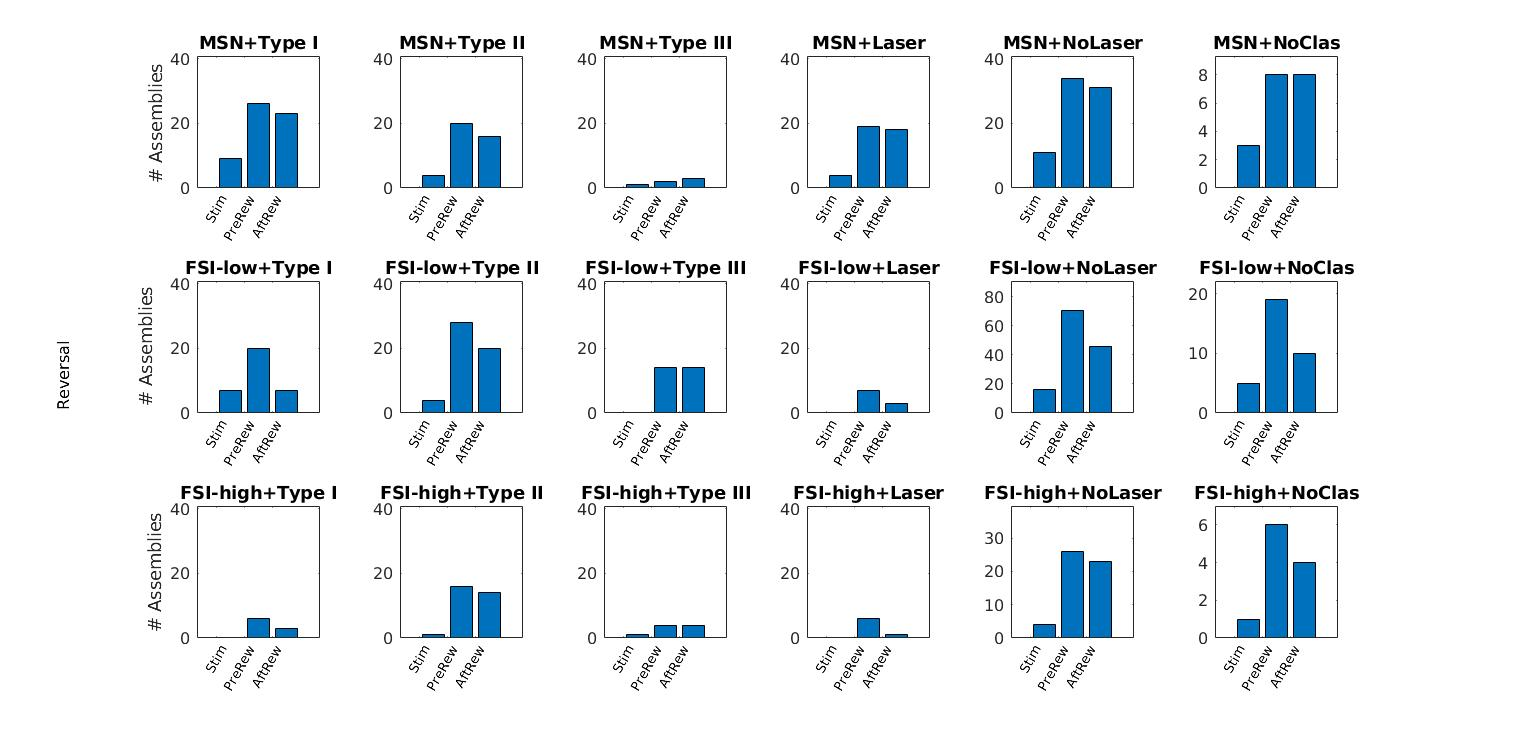
\includegraphics[scale=0.3]{figures/Reversal_Hit_N.jpg}
     %\caption{{\color{red}TO MODIFY!!!! BUT THIS IS THE PLOT}}
     %\label{fig:histo_taskrel}
 %\end{figure}
%\begin{figure}
  %  \centering
   % 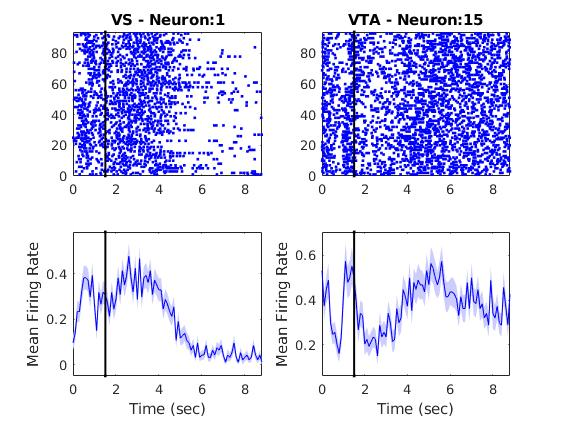
\includegraphics[scale=0.6]{figures/SingleNeus1_15Lastrev1Pru_An_4.jpg}
    %\caption{Shift in time of neuronal activity of two units in assembly. }
    %\label{fig:NeusInAsse}
%\end{figure}

%\section{Discussion}
%\section{Combination of single neuron and assemblies analysis}
%\subsection{Directionality using classification}
%\subsection{Significant task related response for typology}
%%%%%%% Fine Commento forse da buttare


%%%%% Commento Utile
%To better study assemblies activation patterns, first the task relevant moments of the experiment were selected. From the mean task related activity patterns we expected to see differences among assemblies types in two experimental chapters (original and reversal). To better visualize the task related activation patterns via heat plots, hit trials (rewarded odor, mouse went for reward), correct rejection trials (unrewarded odor, mouse sat quiet), false alarm trials (unrewarded odor, mouse went for reward), were kept separated; however this separation among trials types was released in further analysis, without affecting results.
%The assemblies were pruned according their significant task related activity, that was tested with Friedman's test and a non parametric version of the repeated measures Anova. We preferred to use non-parametric tests to be free from the assumption of gaussianity of the observations. Results of the two tests were consistent each other. The two relevant events of the task were the odor onset and the reward delivery, then we choose whether the assemblies showed a significant activity in three windows: Stimulus [0s, 0.5s], Pre-Reward [-0.5s, 0s], Reward [0s, 05s], the baseline was chosen in the interval [-1s, -0.5s] from the odor onset. Post-hoc analysis were performed using the Bonferroni's criterion {\color{red}check whether the criterion was Bonferroni of some other}. Almost $80\%$ of the VS-VTA assemblies showed a task related activity significant different from the baseline or from another of the windows considered. Of the significant assemblies $\%$ were composed by MSN-Type I units, $\%$ by FSI low-Type I, $\%$ by FSI high-Type I, $\%$ MSN-Type II, $\%$ by FSI low-Type II, $\%$ by FSI high-Type II, the other possible units combinations constitutes a minority and all toghether were the $\%$ {\color{red} Insert numbers of percentage}.

%\section{Conclusion}

%\chapter{Reinforcement Learning Model}
\label{chap:RLModel}
\section{Introduction}
In the last session we analyzed the task-related activity patterns of principal assembly-pair types.\\Significant task related activity was tested with Friedman test in stimulus presentation (CS+/-) interval, stimulus continued\footnote{The window right before the reward delivery time, or the expected reward time in False Alarm trials, or the hypothetical reward time in Correct Rejection trials.} (CS+/- cont.) interval, and reward\footnote{Or expected reward in False Alarm trials, or Hypothetical Reward in Correct Rejection trials.}.\\We found a good portion of SPN-DAN pairs becoming active early at stimulus presentation, another important group being active later during the stimulus presentation, and only a small fraction of SPN-DAN pairs active only at the retrieval.\\The described activity pattern makes SPN-DAN pairs good candidates for reward prediction (RP) and reward prediction error (RPE) coding.\\On the other hand we observed that FSN-DAN pairs are early activated by the stimulus on onset and they phasic activate at the reward time.\\While in False Alarm a good portion of FSN-DAN is depressed before and after the expected reward time. Such activity could reflect motivational feelings of the animal during the task, that are partially involved in the reward prediction error definition.\\The analysis of task related responses cannot read the highly dynamic of task, the task was indeed such that the animal had to assign and re-assign a value to the rewarded odor to be able to predict the reward. Only taking in account this dynamic we can understand whether and how SPN-DAN and FSN-DAN pairs compute reward prediction error, and if different cell-assembly types specialize in different aspects of the complex task-related coding.\\To take all this into account, we used the reinforcement learning technique \cite{SuttonBarto}. $"$Reinforcement learning$"$ is an area in machine learning, in which an agent tries to learn the best action to take, depending on the circumstances in which this action will be performed, this approach can incorporate any changes in the environment of the decision making process. In psychology, from where the idea of this machinery derives, the concept is known as “learning by reinforcement”: the agent receives a reward or punishment, depending on the decision made, through the experience he is able to associate the actions that generate the greatest reward for each situation that the environment presents, and to avoid unrewarded actions or actions that generate punishment.\\
Machine learning uses the same idea: the machine observes a state and, based on this, chooses an action to take and receives the reward associated with that specific action in that state, thus obtaining the information of this specific combination. The process is repeated until the machine is able to choose the best action to take for each of the possible scenarios to be observed in the future.\\In the contingencies of the experiment conducted in our lab, two odor were presented and only one was associated with a reward with a probability of 0.9. Each time one odor was presented the mouse chose to take the action (lick or not lick) that maximized the reward and minimized his effort. the task was learnt when the animal was able to lick for the rewarded odor and not lick when the unrewarded odor was presented.\\To model this learning process we set up a Rescorla Wagner model with Pearce Hall update mechanism (\cite{Li}, \cite{Costa}, \cite{Koppe}).\\

%%
%We use here Reinforcement Learning/Forgetting models (\cite{SuttonBarto}) with Q-learning values (\cite{Dayan1}) to fit mice behaviour in go-no go odor discrimination task; we regress afterwards neuronal activity with model values.
\section{Model}
%%%%%{\color{blue}Start writing equation of reinforcement learning}
%%%%%First Option I tried, Georgia's option {\color{red}cite Georgia's paper}
%%%%%We set up four RL models and we chose the one that better fitted the behaviour for the regression analysis.
Reinforcement learning model are usually set up as follows:
\begin{itemize}
    \item At each trial $t$ of the experiment, a state $s$ is observed, this is an input of the model.
    \item After the stimulus presentation, the animal has the chance to take an action, and according to choice made, the reward is delivered. The reward is a vector $r(t)$, each vector component indicates the reward value delivered at the trial $t$, the reward vector is an input of the model.
    \item After the reward delivery, the animal computes the reward prediction error, that is evaluated in the model as the difference between the actual reward and the expected reward.
    \item States values are the expected reward values and they are updated according to the last expected values and the reward prediction error and it is modulated by the learning rate.
    \item The learning rate is often a constant free parameter, however it has been shown that a time dependent variable better describes the learning dynamic (\cite{Funamizu}, \cite{Daw}).
    \item Learned values are then translated into action probabilities via a softmax function, maximized with respect some free parameters.
\end{itemize}

We set up a Q Learning-Forgetting model (Q L-F model) starting from an hybrid Rescorla-Wagner/Pearce-Hall update mechanism (\cite{Koppe}, \cite{Costa}, \cite{Li}) with update of unchosen option (\cite{Katahira}) and the associability related to the chosen and unchosen options, using learning and forgetting parameters ({\color{red} cite Dayan, literature on Q L-F models}).
The model assigns each state $s$ and action $a$, an action value $Q_{s,a}(t)$ where $t$ is the index of the trial. In our specific case we have two states, corresponding to the two odors presented and two possible actions, i.e., to lick or not to lick. 
Based on the set of action values the model transforms the The action value for the chosen option is updated by
\begin{equation}
Q_{s,a}(t+1)  = Q_{s,a}(t)+k_L\cdot\alpha_L(t)\cdot\delta(t), \hspace{0.3cm} with \hspace{0.3cm}\delta(t)=r(t)-Q_{s,a}(t)
\label{eq:Qlearning}
\end{equation}
where $\delta$ is the prediction error, i.e., the difference between the reward $r(t)$ and the expected reward value $Q_{s,a}(t)$ for an action $a$ given a state $s$, $k_L$ is the learning parameter and $\alpha_L(t)$ is the Pearce-Hall associability for the chosen option, is a trial-dependent rate component which adjusts in accordance with the average accuracy of recent predictions, evolving by
\begin{equation}
   \alpha_L(t)=(1-\eta)\cdot\alpha_L(t-1)+\eta\cdot\abs{\delta(t)},\hspace{0.3cm} \eta\in[0,1]
    \label{eq:Alphalearning}
\end{equation}
Note that the $n$'s associability depends on absolute prediction errors from past trials, but not the current one ensuring that $\delta(t)$ was not double counted in the value update.\\The associability term in eq. \ref{eq:Alphalearning} measures the attention that the animal has to put to the cue, in other terms it is nothing but the uncertainty of the animal to get the reward. 
For the unchosen option $a'\neq a$ the action value is updated by
\begin{equation}
    Q_{s,a'}(t+1) = Q_{s,a'}(t)-k_F\cdot\alpha_F(t)\cdot Q_{s,a'}(t)
    \label{eq:Qforgetting}
\end{equation}
where $k_F$ is the forgetting rate (\cite{ItoDoya}) and the associability for the unchosen option is time-dependent and evolves as follows
\begin{equation}
    \alpha_F(t)=(1-\eta)\cdot\alpha_F(t-1)+\eta\cdot Q_{s,a'}(t-1), \hspace{0.3cm}
    \eta\in[0,1]
    \label{eq:Alphaforgetting}
\end{equation}
Note that using $k_F = 0$ the model is reduced to the basic Rescorla Wagner/Pearce Hall model. We applied to our data four different version of the model, the one shown here as presentation is the one that better fit the behavioural data. The other three versions are:
\begin{description}
    \item[i.] \textbf{Rescorla-Wagner.} The presented model is reducible to an hybrid Rescorla Wagner/Pearce Hall update mechanism when we use a learning parameter $k$, and no forgetting parameter, i.e. $k_F = 0$.
    Then, if $a$ represents the chosen option and $a'\neq a$ the unchosen option, the action values evolve as follows\\
    $\begin{array}{lcl}
    Q_{s,a}(t+1)&=& Q_{s,a}(t)+k\cdot\alpha_L(t)\cdot\delta(t), \hspace{0.3cm} with \hspace{0.3cm}\delta(t)=r(t)-q_{s,a}(t)\\
    Q_{s,a'}(t+1)&=&Q_{s,a'}(t)\\
    \end{array}$
    \item[ii.] \textbf{Rescorla-Wagner with two learning rate modulations.} Let $a(t) \in \{1,0\}$ denote the option was chosen at trial $t$, where $1$ stands for "to lick" and $0$ stands for "not to lick". We introduce then two learning parameters $k_{1}$ and $k_{0}$ respectively for the choice $a=1$ and $a=0$ to be estimated by the model, while $k_F$ is fixed to zero.
    Then when the choice $a=1$ is realized, the action values evolves by\\
   $\begin{array}{lcl}
       Q_{s,1}(t+1)&=&Q_{s,1}(t)+k_1\cdot\alpha(t)\cdot\delta(t)\\
         Q_{s,0}(t+1)&=&Q_{s,0}(t)\\ 
    \end{array}$\\
    while if the choice $a=0$ is realized we have\\
    $\begin{array}{lcl}
       Q_{s,0}(t+1)&=&Q_{s,0}(t)+k_0\cdot\alpha(t)\cdot\delta(t)\\
         Q_{s,1}(t+1)&=&Q_{s,1}(t)\\ 
    \end{array}$
    \item[iii.] \textbf{Rescorla-Wagner with two $\eta$ parameters.} We use a learning model, without forgetting parameters, and we introduce two $\eta$ parameters $\eta_1$ and $\eta_0$ for the choice $1$ and $0$ respectively, to be estimated by model. The associability $\alpha_L$ evolves as follow:\\
   $\begin{array}{lcll}
    \alpha_{L}(t) & = & (1-\eta_1)\cdot\alpha_{L}(t-1)+\eta_1\cdot\abs{\delta(t)} & \mbox{if\,\,}  a=1,\\
    \alpha_{L}(t) & = & (1-\eta_0)\cdot\alpha_{L}(t-1)+\eta_0\cdot\abs{\delta(t)} & \mbox{if\,\,}  a=0.\\
    \end{array}$\\
    and action values for the chosen option evolving consequently as in the equation \ref{eq:Qlearning}.
\end{description}
\section{Goodness of Fit}
\label{sec:Behavior}
The hybrid Rescorla-Wagner model (i.) has fewer parameters with respect to the three adapted Rescorla-Wagner versions proposed (ii.,iii., L-F model), and all the three versions can be transformed to the hybrid Rescorla-Wagner by imposing constraints on the former's parameters. Thus using Likelihood Ratio tests for nested models we could test for each alternative model proposed whether it was better than the hybrid Rescorla-Wagner.({\color{red}insert reference})Likelihood ratio test (LRT) is formalize as the ratio of the likelihood functions of the models to compare: 
\begin{equation}
LRT = -2 \log (\frac{\mathcal{L}_s(\hat{\theta})}{\mathcal{L}_g(\hat{\theta})})
\label{eq:LRT}
\end{equation}
where $\hat{\theta}$ are the parameters values that maximize the likelihood function.
The simpler model (s) has fewer parameters than the general model (g), the latter can be reduced to the simpler model after imposing some constraint (null hypothesis).\\
LRT compares the fit of two models and has an asymptotic $\chi^2$ distribution. The null hypothesis is that the smaller model is the $"$best$"$ model.  The null hypothesis is rejected when the test statistic is large. In other words, if the null hypothesis is rejected, then the larger model is a significant improvement over the smaller one.\\
In this way in each test we tested whether the addition of one parameter to the pure Rescorla-Wagner model was needed and brought an improvement. The tests were conducted separately for each animal.\\In the comparison between the Rescorla-Wagner and the Learning-Forgetting, the second model reveals to be the $"$best$"$ model for each animal.{\color{red}show pvalues in a tables}
A further test was needed to understand whether the Learning-Forgetting was the best model among the three adapted version of the hybrid Rescorla-Wagner. In this case the best model was evaluated using the Bayesian Information Criterion (BIC), that is is a criterion for model selection among a finite set of models where the model with the lowest BIC is preferred. BIC is formally defined as (\cite{Schwarz})
\begin{equation}
    BIC=k\log(n)-2\log(\hat{\mathcal{L}})
\end{equation}
where:
${\hat{\mathcal{L}}}$ is the maximized value of the likelihood function of the model, $n$ is the sample size, $k$ is the number of parameters estimated by the model.
Following Raftery’s approach, we considered that a difference of BIC lower than 2 between two models is barely worth mentioning, a difference between 2 and 5 is positive, a difference between 5 and 10 is strong, and a difference larger than 10 is very strong (\cite{Raftery}).\\
From the Bayesian Information Criterion (BIC) the L-F model resulted to be the best model fig.(\ref{fig:BIC}), confirming the evidences of the action values plots in fig.(\ref{fig:PerfRL}).
{\color{red}Missing: BIC PLOT. Proper BIC discussion!!! }
%\begin{figure}
 %   \centering
 %   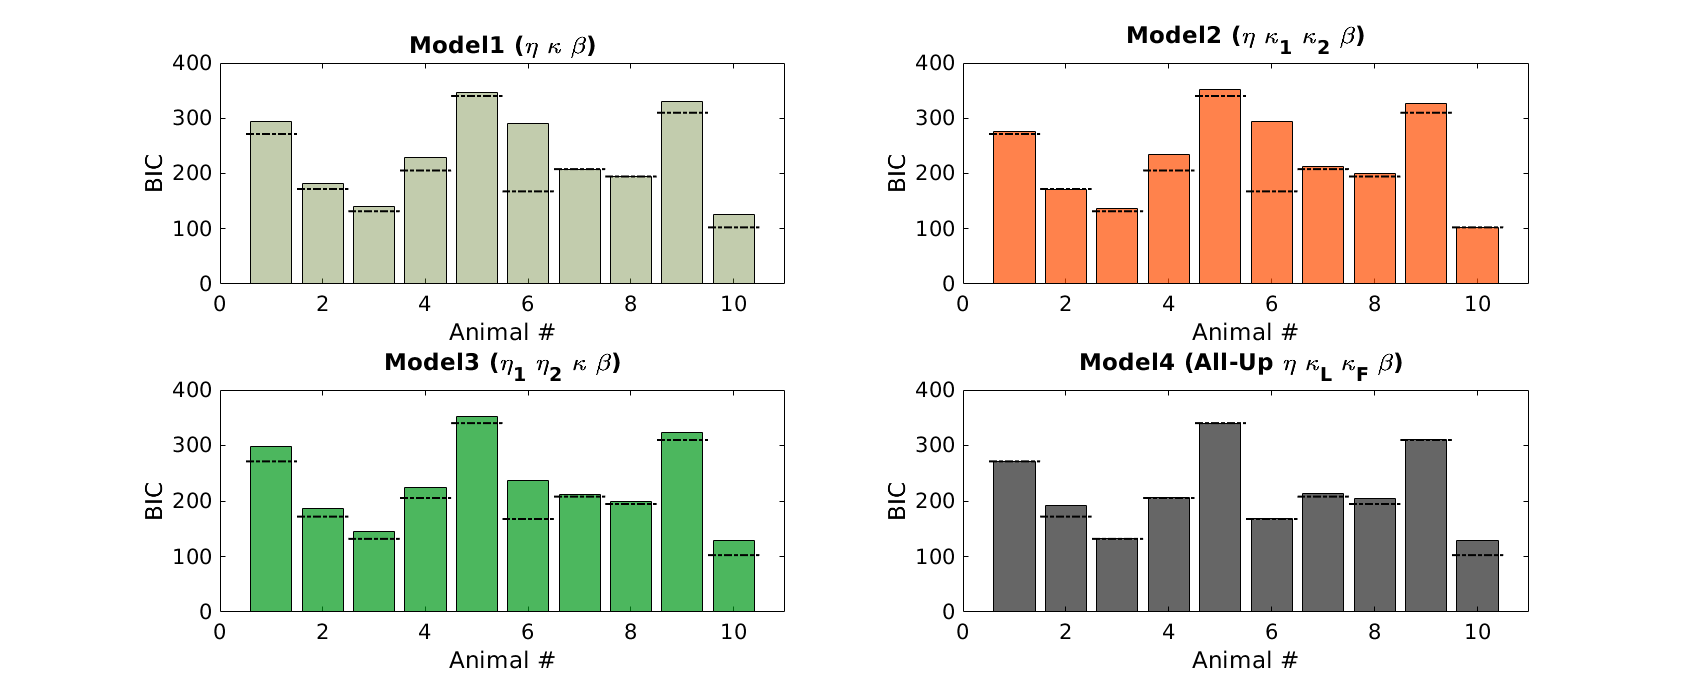
\includegraphics[scale=0.6]{figures/BIC_ModelCompare.png}
 %   \caption{{\color{red}Change figure and title of the plots} BIC Information Criterion for the four models implemented}
 %   \label{fig:BIC}
%\end{figure}
\begin{figure}
\centering
    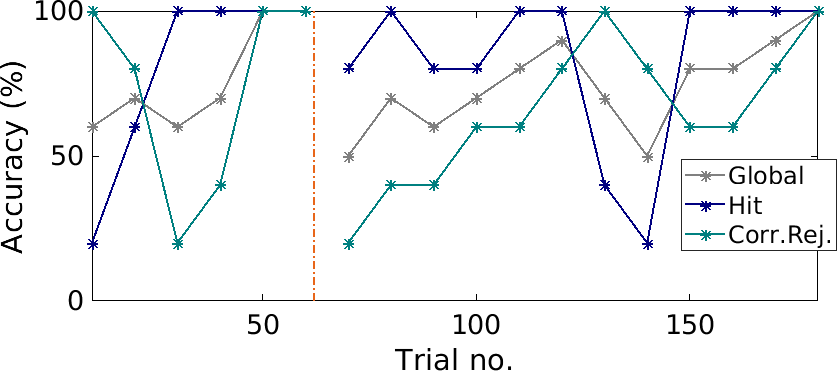
\includegraphics[scale=0.42]{figures/PerfEndrevAn1.png}
    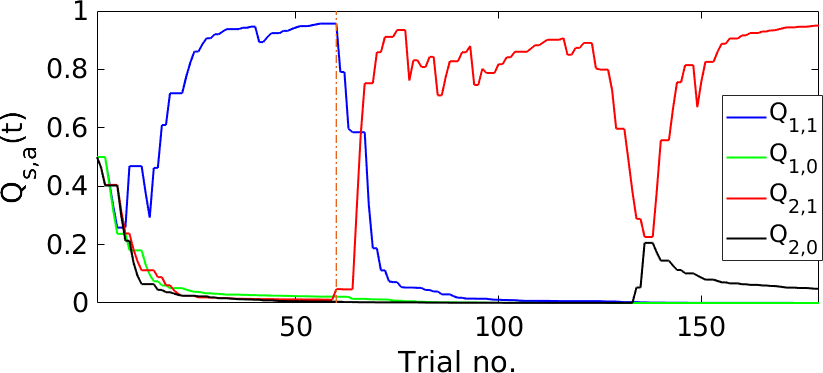
\includegraphics[scale=0.42]{figures/QValuesEndrevAn1.png}
    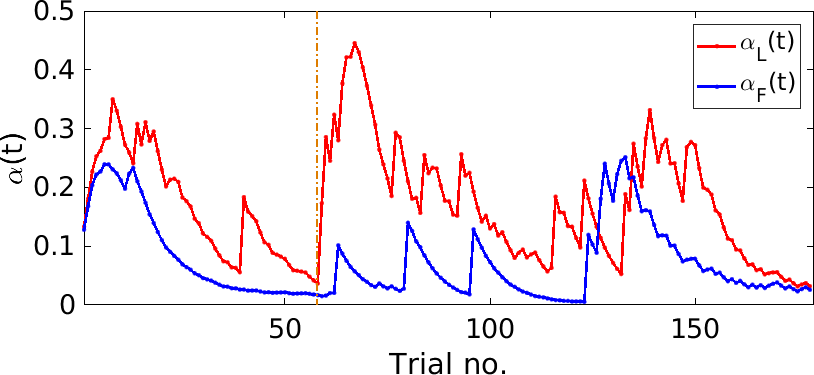
\includegraphics[scale=0.42]{figures/AlphaEndrevAn1.png}
    \includegraphics[scale=0.42]{figures/DeltaEndrevAn1.png}
    \caption{In figure one example of animal performance and RL model action values.
    Odor 1 was rewarded only in the original phase, while Odor 2 was rewarded only in the reversal phase. Top: Performance in all trials, in hit trials and correct rejection trials. Bottom: RL model action values for the action lick, when odor 1/odor 2 occurs (blue/red) and the action no lick when odor 1/odor 2 is presented (green/black).}
    \label{fig:PerfRL}
\end{figure}
In figure one example of animal performance and RL-models action values. When the odor is rewarded the expectancy of reward related to the lick action reproduce the hit performance as one could intuitively predict, while, for non rewarded odor, the reward expectation associated to the no-lick action decrease as the correct rejection performance increase. Action values associated to lick for non rewarded odor and non-lick for rewarded odor give us an estimation of $"$false alarm$"$ and $"$miss trials$"$, namely respectively trials in which the odor was not rewarded and the mouse went for the reward, or in which the odor was rewarded and the mouse sat quiet. That happened especially as the experiment or the new phase began for the first 5-10 trials of the phase.\\

To see whether the neural activity is correlated with the behaviour, we regress the neuronal activity and the assembly activity with the Q L-F model action values $Qs$, error prediction $\delta$, and associability $\alpha$ and behavioural measures. 
    
\section{Uncertainty and prediction error signal in pair-types}
\label{sec:CorrRL}
We assume VS-VTA interactions being able to predict the reward and compute prediction error. We used a reinforcement learning model to parameterize the learning functions, if the assembly-pairs code for some aspects of the learning they correlate with some reinforcement learning functions.\\
In \hyperref[sec:TaskResp]{~Section \ref*{sec:TaskResp}} we hinted which kind of trial variability in assembly activity we expect when the assembly predicts the reward and computes prediction error, doing a parallelism with the dopamine neurons response in case of probabilistic reward \cite{Fiorillo}.\\
An intuitive way to use the task variability to see the correlations with model functions consists in dividing the task in two phases: a first phase constituted by first trials in which we think the animal is learning the task and is uncertain about the reward outcome, we call this phase the unstable phase; a second phase is on the other hand constituted by last trials of the task in which the animal has learnt the task rule and it is more certain about the reward outcome when a rewarded or unrewarded odor is presented.\\
If the assembly-pairs activity codes for the reward prediction we expect intense activity in the CS window during the stable phase, when the animal is able to predict the reward, this case in the probabilistic reward comparison is similar to the case in which the probability to get the reward is equal to 1 or high (see fig. \ref{fig:RewPred} top); whereas during the unstable phase we expect few activation in CS window because the animal is uncertain to get the reward, this case sis comparable with the case of reward probability equal to 0.25 or below (see fig. \ref{fig:RewPred} bottom). In other words we expect the assembly-pair activity in CS window to anti-correlate with the uncertainty $\alpha_L(t)$, indeed the uncertainty is high at the beginning of the task and goes down at the end of the original phase, to raise up again at the beginning of the reversal phase. In fig. ({\color{red} metti una figura, quella usata all'embl}) we compare the assembly-pairs activity in unstable and stable phase. The difference between the two phase is significantly different from zero only for SPN-DAN pairs.\\
With similar arguments we can assume that, if the assembly-pairs compute reward prediction error their activity should correlate with the prediction error $\delta(t)$ in the US window.
%We carried out a multiple regression analysis of neuronal and assembly's activity by the four action values of the Q F-L model, $\delta(t)$, $\alpha_L(t)$ and $\alpha_F(t)$. To further test whether the neuronal and assembly activities were correlated with the parameters of subsequent lick movements, or the odor identity, we analyzed the residual components, $\epsilon(t)$, using lick related variables and the odor identity, namely, the mouse's action choice $a(t)$, the lick frequency within the lick-window $l_{in}(t)$, the lick frequency outside the lick-window, before the opening,$l_{out}(t)$ and the odor identity $o(t)$.
%Thus we model the neuronal or assembly activity $y(t)$ during the post-stimulus, pre-reward and post-reward periods in the $t-th$ trial as follows:\\
%\begin{equation}
%\begin{cases}
%y(t)=b_0+\sum\limits_{l}^{L} b_l\cdot M_l+\epsilon(t)\\
%\epsilon(t)=\sum\limits_i^I c_i\cdot N_i
%\end{cases}
%\label{eq:MultiLinRe}
%\end{equation}
%where $y$ are the observations, the neuronal{\color{blue}/assembly's} activity in this case, $M$ is the ($T\times L$) regressor's Matrix of the Q L-F model part, where $T$ is the number of trials and $L$ the number of regressors. $M$ has as columns
%the regressors of the model's part, namely, the vectors $Q_{1,1}$, $Q_{1,0}$, $Q_{2,1}$, $Q_{2,0}$, $\delta$, $\alpha_L$, $\alpha_F$; the set of values $b_m$ are regressor parameters or weights related to the model's regressors. $N$ is the ($T\times I$) regressor matrix of the residual part, where $I$ is the number of regressors of the residual part. N has as columns the regressors $a$, $l_{in}$, $l_{out}$ and $o$, while $c_i$ are the weights of the residual part.
%Linear regression models assume response variables to be normally distributed. Neuronal responses are Poisson distributed (although the normal distribution is in this case a good approximation), {\color{blue} and assemblies show Gamma distribution,} thus considering our data distributions, we built a generalized linear model (GLM), with GLM is possible to generalize the simple linear regression by allowing for response variables that have arbitrary distributions and for an arbitrary function of response variables, the link function, to vary linearly with the predicted values, rather than assuming that the response itself must vary linearly. The mean $\mu$ of distributions depends on the independent variables, or the regressors, $X$, as follows:
%\begin{equation}
%E(Y)=\mu=g^{-1}(X\cdot \beta)
%\label{eq:GLM}
%\end{equation}
%where $g$ is the link function. There is always a well-defined canonical link function which is derived from the exponential of the response's density function. For Poisson observation the canonical link function is the logarithmic. Thus the neuronal activities mean can be expressed by the following:
%\begin{equation}
%\begin{cases}
%\log(\mu)=b_0+\sum\limits_l^L b_l\cdot %M_l+\epsilon(t)\\
%\epsilon(t)=\sum\limits_i^I c_i\cdot N_i 
%\end{cases}
%\label{eq:PoisLinRe}
%\end{equation}
\begin{figure}
    \centering
    \includegraphics[scale=0.30]{figures/PreRewDistr_An1neu6_FSI.png}
    \includegraphics[scale=0.30]{figures/PostRewDistr_An1neu6_FSI_.png}
    \caption{Example of one unit firing rate distribution in the pre-reward range [-0.5 s,0s] and during the post reward period [0s,0.5s], choosing as starting time the reward delivery.}
    \label{fig:DistributionEx}\end{figure}
%%%%%%However, in some cases it makes sense to try to match the domain of the link function to the range of the distribution function's mean, or use a non-canonical link function for algorithmic purposes, for example Bayesian probit regression. 
\section{Regression}
\label{sec:Regression}
\section{Conclusion}
%From the regression analysis, as one could predict, VS units emerged to be correlated with the $Q$ values, in particular FSI units show this correlation very clear.


%\begin{figure}
 %   \centering
 %   \includegraphics[scale=0.3]{figures/y_yhatAnimal2neu6_FSI.png}
 %   \includegraphics[scale=0.3]{figures/CorrelationExAn1neu6_RightAx.png}
  %  \caption{Caption}
 %   \label{fig:my_label}
%\end{figure}
%\appendix
%\appendix
\chapter{Appendix A}
\begin{table}[h!]
    \centering
\begin{tabular}{ |p{3cm}||p{3cm}|p{2cm}|p{2cm}| }
 \hline
 \multicolumn{4}{|c|}{Bayesian Information Criterion} \\
 \hline
 Animal & Model & BIC & $\Delta$(BIC)\\
 \hline
\multirow{4}{6cm}{Animal 1} &Model1&BIC1&$\Delta$(BIC1)\\&Model2&BIC2&$\Delta$(BIC2)\\&Model3&BIC3&$\Delta$(BIC3)\\&Model4&BIC4&$\Delta$(BIC4)\\
\hline
\multirow{4}{6cm}{Animal 2} &Model1&BIC1&$\Delta$(BIC1)\\&Model2&BIC2&$\Delta$(BIC2)\\&Model3&BIC3&$\Delta$(BIC3)\\&Model4&BIC4&$\Delta$(BIC4)\\
 \hline
\end{tabular}
\end{table}
%\chapter{Materials and Methods}
\section{Data acquisition}Neural data was recorded with a 64-channel headstage (RHD2164) and interface board (RHD2000) by Intan Technologies LLC at 30 kHz sampling frequency. The same interface was used to record stimulus onset and offset, reward application, licking activity and laser stimulation.
\section{Spike detection}The median voltage trace of the corresponding brain region was subtracted from each recorded trace to reduce noise and movement artifacts affecting all recording sites. The result signal was bandpass-filtered between 300 and 500 Hz. A threshold value for spikes was computed as multiple (7.5x) of the median absolute deviation of the filtered signal ({\color{red}Quiroga 2004- vedere come citare}). To avoid multiple detection of the same multiphasic spike, temporally proximal detected spikes over threshold were pruned by height to a minimum distance of 1 ms. When an event was detected on multiple channels of a tetrode, the timestamp of the highest detected peak was used. Spike waveforms were extracted from -10 to +21 samples around the peak.
\section{Spike sorting}Spike sorting was done with a custom-built graphical user interface in Matlab, using a freely rotatable 3d-point cloud of spike metrics as a basis. Metrics used for clustering included detected peak height or amplitude (and the respective principal components over channels), and the first three principal components of the waveforms for each respective channel when a spike was predominantly recorded on one channel. The quality of single unit clusters was assessed using the mlib toolbox by Maik Stuettgen (version 6, downloaded from Matlab Central) with particular attention to peak height distribution (fraction of lost spikes due to the detection threshold), contamination (fraction of spikes occurring in the refractory period  $\sim$ 5ms) and waveform variance.
\section*{Zusammenfassung}
Ziel vieler Verhalten ist es, das Maß an Belohnung, das erzielt werden kann, zu optimieren. Hierzu muss das Individuum mögliche Vorhersagen über den Zusammenhang zwischen Reizen und Belohnung machen.  Bei diesen Vorhersagen treten natürlich Fehler auf. Vorhersagefehler für Belohnung beschreiben die Differenz zwischen erwarteter und erhaltener Belohnung. Diese Vorhersagefehler sind im Hirn in der Aktivität dopaminerger Mittelhirnneurone in der VTA präsentiert und werden durch belohnte Stimuli und Belohnung hervorgerufen. Diese Dopaminsignale sind essentiell für Lernvorgänge. Insbesondere Modelle des Verstärkungslernens lassen Interaktionen zwischen dopaminergen Mittelhirnneuronen und dem ventralen Striatum (VS) vermuten, die die Differenz zwischen antizipierter und erhaltener Belohnung kodieren. Diese Interaktion konnte bisher aber nicht direkt gezeigt werden.\\In dieser Arbeit untersuchte ich die Entstehung des Vorhersagefehlers in VS-VTA Ensembles während des Verstärkungslernens. Diese Arbeit basiert auf in vivo elektrophysiologischen Untersuchungen im VS -inklusive dem ventralen Pallidum (VP)- und der VTA während einer go/no-go Lernaufgabe in Mäusen. Ich untersuchte insbesondere die Interaktion zwischen VP Neuronen und dopaminergen Neuronen und die zwischen striatalen Projektionsneuronen und dopaminergen Zellen.\\\\Die Analyse der Ensembleaktivität erfolgte mit einem neuen Detektionsalgorithmus. Es zeigte sich hier, dass speziell striatale Projektionsneurone in den Ensembles vor den dopaminergen Mittelhirnneuronen aktiv sind, diese also informieren.\\\\Die Analyse der Ensemble-Aktivität während der Belohnungslernens zeigte ferner, dass Ensembles zwischen striatalen Projektionsneuronen und dopaminergen Neuronen selektiv durch den belohnten Stimulus aktiviert wurden. Demgegenüber zeigten Ensembles mit VP Neuronen eine unspezifische Stimulusaktivierung, was auf eine generelle Kodierung von Stimulussalienz hinweist.\\\\Diese differentielle Aktivierung verschiedener Ensembletypen weißt auf spezifische Funktionen beim Lernen hin. Ich testete diese Frage mit einem Model für Verstärkungslernen basierend auf Rescorla-Wagner Lernregeln, die den Vorhersagefehler und die Unsicherheit der eigentlichen Vorhersage abbilden. In der Tat korrelierte die Aktivität von Ensembles zwischen striatalen Projektionsneuronen und dopaminergen Neuronen mit dem Vorhersagefehler und der Unsicherheit der eigentlichen Vorhersage. Dies trifft nicht auf Ensembles zu, an denen VP Neurone statt den striatalen mit dopaminergen Neuronen interagierten. Zusammenfassend liefern diese Daten direkte Hinweise, dass das ventrale Striatum die VTA über den Vorhersagefehler informiert, der in den interarealen Ensembles zwischen beiden Arealen repräsentiert wird.

\section*{Summary}
Reward is an object, stimulus, situation or activity that evokes positive emotions such as pleasure and desire. Hence, during learning or in decision making processes, agents behave in such a way to maximise the reward. Maximisation of the reward requires prediction, namely information about the future. An error can be defined in the most general sense as a discrepancy between what is happening and what is predicted to happen. A reward prediction error, then, is the difference between a reward that is being received and the reward that is predicted to be received. Thus, reward prediction error signals are essential to learning and they are supposed to be encoded by dopamine neurons through dopamine pathways. In particular the mesolimbic dopamine pathway comprising the ventral tegmental area (VTA) and projection terminals in the ventral striatum (VS) has been identified as a critical neural system involved in processing reward prediction error. In this thesis we proposed a study of formation of reward prediction error signals in VS-VTA interregional assemblies during learning. We recorded in-vivo electrophysiological data in VS - including ventral pallidum (VP) - and VTA, during a reversal go/no go task in mice. VS/VP units were classified in striatal projection units (SPN), fast spiking neurons (FSN) and cholinergic interneurons (CIN), whereas VTA units were classified in dopamine neurons (DAN), gabaergic neurons (GABA) and glutammatergic neurons (GLU). On this data set we applied a novel cell-assembly detection method able to detect assemblies of synchronously ($lag=0$) and sequentially ($lag\neq0$) active units at arbitrary time scales ($\Delta$). The temporal precision of assemblies detected across VS-VTA displayed a bimodal distribution with peaks around hundred milliseconds and one second. Interestingly the lags of more temporally precise assemblies displayed an asymmetric distribution indicating VS leading VTA. Specifically, these directional assemblies were composed of SPN leading DAN.\\Analysing the task related activity of the detected cell assembly-types, we found that the activation of assemblies with SPN and DAN was led by the rewarded stimulus, while only few of them were activated by the unrewarded stimulus. Whereas assembly with FSN and DAN neurons could be either activated or inhibited in response to one or both signals. Such patterns suggested that SPN-DAN assemblies were involved in reward prediction error coding while FSN-DAN assembly showed motivational and/or hedonic salience. In this way we assumed that different assembly types in the VS-VTA circuit specialized in different coding features during learning. We formally tested this hypothesis with reinforcement model using the Rescorla-Wagner learning rule, whose crucial terms were the reward prediction error and the uncertainty to get the reward. Based on broad knowledge, reward prediction error signals are assumed to anticorrelate with the uncertainty at the stimulus presentation, and to correlate with the reward prediction error term. The SPN-DAN assemblies indeed are anticorrelated with the uncertainty and correlated with the prediction error; thus they convey the prediction signals, crucial to learning. Furthermore we found that this encoding feature is not present in other assembly-types, confirming the hypothesis that different pathways of the VS-VTA circuit specify in different reward-related signals.
\chapter{Introduction}
\label{chap:Introduction}
%\section{Motivation}   
%\label{sec:Motivation}
The mesolimbic dopamine pathway comprising the ventral tegmental area (VTA) and projection terminals to the ventral striatum (VS) has been identified as a critical neural system involved in processing both the rewarding and aversive behavioral effects of rewarded and unrewarded stimuli (\cite{Schultz1992}, \cite{Montague}, \cite{Ungless2004}, \cite{Sun2014}, \cite{Tobler2003}, \cite{UchidaDop1}, \cite{Takahashi2016}). In these functions the brain performs simple arithmetic: it compares the expected and the received outcomes and computes the differences between the two. In other words after receiving the outcome, it computes the error made in predicting the outcome. This signal is called reward prediction  error (RPE): being essential to learning, to reward maximization, and to guide reward-related behavior, RPE has been widely investigated in last decades (\cite{Schultz1997},, \cite{UchidaDop}, \cite{Fiorillo}, \cite{Pagnoni}, \cite{Schultz2016}). In dopamine neurons RPE signals are characterized by activations following primary food and liquid rewards, and visual, auditory and somatosensory reward-predicting stimuli. Dopamine neurons fire phasically (100-500 ms) after unpredicted rewards or cues that predict reward. Their response to reward is reduced when a reward is fully predicted (\cite{Uchida}). The uncertainty about the reward outcome is critical in the measure of information and in assessing the accuracy of predictions. The uncertainty is determined by the probability P to get the reward, and its maximal at $P=0.5$, while decreases at higher and lower probabilities.\\Fiorillo and collaborators used distinct stimuli indicating the probability of reward, to show that the phasic activation of dopamine neurons varied monotonically across the full range of probabilities (\cite{Fiorillo}). Figure \ref{fig:probDopamine} (left) displays the dopamine neurons response to stimuli with different reward probability. These observations have defined the basis of the current knowledge on dopamine neurons, which are assumed to signal discrepancies between expected and actual rewards, in other words they are thought to compute the reward prediction error (RPE).\\Being essential to learning, since ever RPE signals picked the scientist$'$ curiosity, who dissected the evolution in time of those signals to understand the underlying nature of multiple time components of RPE. The reward-related activation is usually preceded by a brief detection component before the proper valuation of stimulus: the RPE signal evolves in time from unselective sensory detection to more demanding and crucial stages of identification and valuation (\cite{Tobler2003}, \cite{Nomoto2010}, \cite{Fiorillo2013}, \cite{Schultz2016}), value that is constantly adapted during the learning process by dopamine neurons (\cite{Tobler2005}). The initial component, characterized by a brief activation, occurs unselectively in response to a large variety of unpredicted events and corresponds to the large range and heterogeneous nature of potentially rewarding stimuli and object present in the environment.
\begin{figure}[H]
    \centering
    \includegraphics[scale=0.6]{figures/Schultz1.png}
    \hspace{1.5cm}
    \includegraphics[scale=0.35]{figures/ResponseProbSchultz.png}
    \caption{\textbf{Left:} Adapted from \cite{Fiorillo}: Reward-related responses of dopamine neurons. Distinct stimuli were used to indicate the probability of reward (p increasing from top to bottom). Dopamine neurons signals varied monotonically across the full range of probabilities. At the stimulus onset, the dopamine response increased monotonically as the probability increased; at the reward time instead, the dopamine response decreased monotonically as the probability increased. \textbf{Right:} Adapted from \cite{Schultz2016}: A demanding random dot motion discrimination task reveals completely separated dopamine response components. Larger responses correspond to higher reward probabilities (p). The initial, stereotyped, non-differential activation reflects stimulus detection and decreases back to baseline (blue zone); the subsequent separate, graded increase develops when the animal signals stimulus discrimination; it codes reward value (red zone), which in this case derives from reward probability}
    \label{fig:probDopamine}
\end{figure}
This component reflects the detection of stimulus, regardless its relation with the reward.\\The second component, also called main component or valuation component, defines the function of the dopamine response and reflects the evolving neuronal processing that is required to fully appreciate the value of the stimulus. Thus, at this stage the stimulus is identified and valued. Figure \ref{fig:probDopamine} (right) shows the separation between the detection salience and the valuation component of RPE signals in dopamine neurons.\\Like VTA neurons, VS neurons show as well reward-related response. In monkey experiments first it has been shown that VS neurons predominantly fire in relation to the expectation of reward, regardless of the movement/no-movement reaction (\cite{Schultz1992}). This signals suggested that VS neurons evaluate reward and reward-associated stimuli, and thereby participate in the processing of information underlying the RPE computation.\\The stereotypical responses of striatal projection neurons in VS during learning consist of a sustained increase of activity before the occurrence of the reward delivery (see figure \ref{fig:StriatumN}).
\begin{figure}[H]
    \centering
    \includegraphics[scale=0.22]{figures/StriatumR.png}
    \caption{Adapted from \cite{Schultz1992}. Stereotypical reward-related VS neuronal activity. Effect of delayed reward delivery in no/ no go task in monkeys. VS neurons show sustained increases of activity before the occurrence of individual task events. VS neurons exhibit activation in relation to the expectation of reward.}
    \label{fig:StriatumN}
\end{figure}
The ventral pallidum (VP), from which neurons with fast spiking activity were recorded, is innervated by dopamine inputs from the midbrain and dopamine directly alters VP neuronal firing (\cite{Napier89}). Since 1991 VP was assumed to integrate reward-related signals carried by VTA dopamine neurons, involved in reward-motivated behavior (\cite{Napier91}). This concept was quickly expanded to encompass the idea that dopamine transmission within the VP regulates a collection of behaviors, including locomotion and cognition (\cite{Napier92}). Contrary to the well-characterized, relatively homogeneous projection neurons dominating striatum, the cellular architecture of VP is only beginning to be understood in terms of their heterogeneous cell-types, neurotransmitters, and connectivity (\cite{Heimer1997}, \cite{Tachibana2012}). In other studies conducted in our lab, it was observed that VP units displayed either purely excitatory, purely inhibitory, or multiphasic excitatory and inhibitory responses to the same stimulus or across reward and unrewarded stimuli (unpublished results). For these reasons, the responses of VP neurons are expected to be diverse among different VP units.\\While there exist an extensive literature on how RPE signals are expressed by single units, how the RPE computations are implemented in VS-VTA neural circuits remains elusive. Thus, better understanding VS-VTA related circuits, will broaden our understanding on the underpinnings of RPE signals.\\In this work I studied the formation of prediction error signals in interregional assemblies during reinforcement. Towards this aim, I used dual site electrophysiological in-vivo data from VS (including ventral pallidum) and VTA, during a reversal go/no go task in mice.\\On this data set I applied a cell assembly detection algorithm (\cite{RussoDurstewitz}). The novel statistical approach was built to detect spike patterns at any time scale and coordination, enabling so the investigation of the time scales and the inter-units lag activation involved in the detected patterns of spikes. I focused the analysis on interregional assembly-pairs, namely assembly formed by two neurons, one in VS and the other in VTA. In this way I were able to examine the directionality between VS-VTA interactions through the inter-unit lag activation.\\I found that, in interregional assembly-pairs, VS predominantly led VTA. Moreover interregional assembly-pairs showed a bimodal time scale distribution, such bimodality was solely present in VS-VTA pairs and did not emerge in intraregional pairs.\\I examined the assembly-pair activity patterns of pairs with different time scales and directionalities. It emerged that different time scales and directionalities segregated different activity patterns. Specifically, in more precise time scale, directional assembly-pairs with VTA following VS showed excitatory responses following reward-predicting stimuli, in agreement with prediction error encoding.\\Taking advantage of neuron types classifications both in VS and VTA, I further investigated the specific cell-type composition of the assemblies exhibiting directionality. Interestingly only assembly-pairs formed by putative striatal projection neurons (pSPN) and dopamine neurons (pDAN) were directional in the direction of VS leading VTA.\\Thus, I looked at the task related activity patterns of different assembly-pair types; and I expected that, being directional, SPN-DAN assembly-pairs could exhibit RPE response.\\Indeed, different assembly-pairs types showed different activity patterns in response to external potentially rewarded stimuli. The segregation reflected different encoding features in different assembly-pair types.\\In particular, SPN-DAN assembly-pairs were mainly activated by the rewarded stimulus, and only a small fraction ($\sim12\%$) was activated by both stimuli. The activation started few hundred milliseconds after the stimulus onset and remained high for few hundred milliseconds ([100,400] ms). SPN-DAN activity pattern suggested that those pairs conveyed the valuation component of RPE signals (\cite{Tobler2003}, \cite{Nomoto2010}, \cite{Schultz2016}). Conversely, FSN-DAN assembly-pairs responded indistinctly to both stimuli, either showing a brief and phasic activation at the stimulus onset or being inhibited by one or both stimuli; these signals suggested that FSN-DAN pairs were involved in motivational and/or hedonic signals. Hence, I put forth the hypothesis that the assembly-pairs specialize in different aspects of the learning-related coding.\\%\\Detailed discussion will be presented in\hyperref[sec:TaskResp]{~Section \ref*{sec:TaskResp}} and\hyperref[sec:FalseAlCorrRej]{~Section \ref*{sec:FalseAlCorrRej}}.\\
So far the description barely considered the dynamic of the learning process. In fact, reward prediction coding signals in dopamine neurons varied according to the probability to get the reward, which was often related to the uncertainty (\cite{Schultz1992}). Dopamine neurons in VTA as well as neurons in VS modified their activity in function to the difference between received and expected outcomes (\cite{Fiorillo}). In similar ways, far from being static, the assembly-pair activity modified itself trial by trial, reflecting the dynamic of the learning.\\This dynamic could not be replicated by the study of activity patterns, for this reason I modeled a reinforcement learning model. Crucial terms of reinforcement learning are the uncertainty of the animal to get the reward and the reward prediction error; the first is high when the animal is unsure about the outcome, and decreases as the animal becomes expert; the latter term reflects the ability of the animal to predict the reward: as the animal learnt is supposed to be able to predict the future outcomes. Both the aforementioned terms were modeled as time evolving components, in such a way that I could take into account the fact that, during the task, the animal had to assign and re-assign new value to the presented stimulus.\\Based on broad knowledge, reward prediction error signals are thought to be anti-correlated with the uncertainty of the animal to get the reward and correlated with the prediction error term of the Rescorla-Wagner models.\\Thus, if SPN-DAN assembly-pairs specifically encoded prediction error signals, I expected their activity to anti-correlate with the modeled uncertainty ($\alpha$) and to correlate with the modeled prediction error ($\delta$).\\Imodeled two linear Poisson regressions and I regressed the assembly-pairs activity on $\alpha$ and $\delta$. Our SPN-DAN assembly-pairs indeed anti-correlated with the uncertainty and correlated with the prediction error term. Furthermore I noted that such correlations were not found in other assembly-pair types, from which I could conclude that SPN-DAN assembly-pairs specifically conveyed reward prediction signals.  
\chapter{Overview}
\label{chap:Overview}
\section{State of the art}
\label{sec:StateArt}
In this section we present the state of the art of the current knowledge of ventral striatum (VS) and ventral tegmental area (VTA), needed for the study of VS-VTA interaction.\\In VTA, dopamine neurons fire phasically (100-500 ms) after unpredicted rewards or cues that predict reward. Their response to reward is reduced when a reward is fully predicted (\cite{Uchida}). %Furthermore, their activity is suppressed when a predicted reward is omitted. From these observations, previous studies hypothesized that dopaminergic neurons signal discrepancies between expected and actual rewards (i.e., they compute RPE).
The uncertainty about the reward outcome is critical in the measure of information and in assessing the accuracy of predictions. The uncertainty is determined by the probability P to get the reward, and its maximal at $P=0.5$, while decreases at higher and lower probabilities.\\Fiorillo and his collaborators used distinct stimuli indicating the probability of reward, to show that the phasic activation of dopamine neurons varied monotonically across the full range of probabilities (\cite{Fiorillo}). Figure \ref{fig:probDopamine} (left) displays the dopamine neurons response to stimuli with different reward probability. These observations have defined the basis of the current knowledge on dopamine neurons, which are assumed to signal discrepancies between expected and actual rewards, in other words they are thought to compute the reward prediction error (RPE).\\Being essential to learning, since ever RPE signals picked the scientist$'$ curiosity, who dissected the evolution in time of those signals to understand the underlying nature of multiple time components of RPE. Several studies have shown that RPE signal evolves in time from unselective sensory detection to more demanding and crucial stages of identification and valuation (\cite{Tobler2003}, \cite{Nomoto2010}, \cite{Fiorillo2013}, \cite{Schultz2016}), value that is constantly adapted during the learning process by dopamine neurons (\cite{Tobler2005}). The initial component, characterized by a brief activation, occurs unselectively in response to a large variety of unpredicted events and corresponds to the large range and heterogeneous nature of potentially rewarding stimuli and object present in the environment. This component reflects the detection of stimulus, regardless its relation with the reward.\\The second component, also called main component or valuation component, defines the function of the dopamine response and reflects the evolving neuronal processing that is required to fully appreciate the value of the stimulus. Thus, at this stage the stimulus is identified and valued. Figure \ref{fig:probDopamine} (right) shows the separation between the detection salience and the valuation component of RPE signals in dopamine neurons. %In stark contrast to the simple models proposed previously, we observed that information about reward and expectation is distributed among multiple brain areas and already mixed in many individual input neurons. Our data suggest that the RPE computation is not a one-step process combining pure information about reward and expectation in dopamine neurons. Nor do dopamine neurons receive complete RPE from a specific brain area. Instead, the coexistence of input neurons encoding pure and mixed information, some of which are partial and complete RPE signals, appears to be a sign of redundant computations distributed in a complex neuronal network that ultimately converge onto dopamine neurons to construct a more complete RPE signal.
\begin{figure}[H]
    \centering
    \includegraphics[scale=0.6]{figures/Schultz1.png}
    \hspace{1cm}
    \includegraphics[scale=0.35]{figures/ResponseProbSchultz.png}
    \caption{\textbf{Left:} Adapted from \cite{Fiorillo}. Reward-related response of dopamine neurons. Distinct stimuli were used to indicate the probability of reward (P increasing from top to bottom). Dopamine neurons signals varied monotonically across the full range of probability. At the stimulus onset the dopamine response increased monotonically as the probability increased, at the reward time instead the dopamine response decreased monotonically as the probability increased. \textbf{Right:} Adapted from \cite{Schultz2016}. A demanding random dot motion discrimination task reveals completely separated dopamine response components. Higher response corresponds to higher reward probability (p). The initial, stereotyped, non-differential activation reflects stimulus detection and decreases back to baseline (blue zone); the subsequent separate, graded increase develops when the animal signals stimulus discrimination; it codes reward value (red zone), which in this case derives from reward probability}
    \label{fig:probDopamine}
\end{figure}
%\begin{figure}
 %   \centering
  %  \includegraphics[scale=0.4]{figures/ResponseProbSchultz.png}
   % \includegraphics[scale=0.4]{figures/Schultz2016CSMod.png}
  %  \caption{Adapted from \cite{Schultz2016}. A demanding random dot motion discrimination task reveals completely separated dopamine response components. Higher response corresponds to higher reward probability (p). The initial, stereotyped, non-differential activation reflects stimulus detection and decreases back to baseline (blue zone); the subsequent separate, graded increase develops when the animal signals stimulus discrimination; it codes reward value (red zone), which in this case derives from reward probability}
 %   \label{fig:probSchultz}
%\end{figure}
Like VTA neurons, VS neurons show as well reward-related response. In monkey experiments first it has shown that VS neurons predominantly fire in relation to the expectation of reward, regardless the movement no-movement reaction (\cite{Schultz1992}). This signals suggested that VS neurons have access to central representations of reward and thereby participate in the processing of information underlying the RPE computation.\\The stereotypical response of projection neurons in VS during learning consists in a sustained increase of activity before the occurrence of the reward delivery (see figure \ref{fig:StriatumN}).
\begin{figure}[H]
    \centering
    \includegraphics[scale=0.22]{figures/StriatumR.png}
    \caption{Adapted from \cite{Schultz1992}. Stereotypical reward-related VS neuronal activity. Effect of delayed reward delivery in no/ no go task in monkeys. VS neurons showed sustained increases of activity before the occurrence of individual task events. VS neurons exhibit activation in relation to the expectation of reward.}
    \label{fig:StriatumN}
\end{figure}
The ventral pallidum (VP), from which we recorded fast spiking activity, is innervated by dopamine inputs from the midbrain and dopamine directly alters VP neuronal firing (\cite{Napier89}). Since 1991 VP was assumed to integrate reward-related signals carried by VTA dopamine neurons, involved in reward-motivated behavior (\cite{Napier91}). This concept was quickly expanded to encompass the idea that dopamine transmission within the VP regulates a collection of behaviors, including locomotion and cognition (\cite{Napier92}). Contrary to the well-characterized, relatively homogeneous projection neurons dominating striatum, the cellular architecture of VP is only beginning to be understood in terms of their heterogeneous cell-types, neurotransmitters, and connectivity (\cite{Heimer1997}, \cite{Tachibana2012}). In other studies we observed that VP units displayed either purely excitatory, purely inhibitory, or multiphasic excitatory and inhibitory responses to the same stimulus or across reward and unrewarded stimuli (unpublished results). For these reason, the responses of VP neurons are expected to be diverse among different VP units, probably depending on the involvement of the unit in a specific coding.
\section{Experiment and data set}
\label{sec:Dataset}
In this session we describe the experiment and the collected data for the analysis in object in this work. The experiment and the single units classification was conducted by Max Scheller, medical student, member of the Kelsch group.\\The task presented is a go/no-go reversal odor discrimination task (see details in \hyperref[sec:MatAndMet]{~Section \ref*{sec:MatAndMet}}).
\begin{figure}[H]
    \centering
    \includegraphics[scale=0.92]{figures/Experiment.png}
    %\includegraphics[scale=1]{figures/Performance.png}
    \caption{Scheme of the experimental setup. Two odors in randomized sequences were presented, the mouse was head-fixed and, to get the reward, had to lick during the allowed licking period when the rewarded odor was presented. Electrodes were implanted in VS (specifically olfactory tubercle -OT-)/VP  and VTA to record the neural activity.}
    \label{fig:experiment}
\end{figure}
In figure \ref{fig:experiment} the scheme of the experimental set-up. Dual-site in-vivo data were recorded in VS (specifically olfactory tubercle -OT-), including VP, and VTA, meanwhile two odors were presented to head-fixed mice, one rewarded (CS+) with reward probability 0.9, the second one unrewarded (CS-). Learning the task consisted in licking at least a defined number of times (two or three depending on the paradigm) during a specific interval, called lick window, when the rewarded odor (CS+) was presented (hit trials) and not licking when unrewarded odor (CS-) was presented (correct rejection trials). Whereas a bad performance consisted in not licking, or licking outside the lick window period, at CS+ presentation (miss trials), or licking at CS- presentation (false alarm trials). Once the performance criterion was reached, the contingencies were switched, in other words the rewarded odor became unrewarded and vice-versa. Once the performance criterion was reached also in the reversal phase the extinction phase followed, in which neither one of the two odors was rewarded. The lick window was open for an interval of a duration ranging between 1500 ms and 2000 ms depending on the paradigm, and it was open only after a delay that could range from 500 ms to 1500 ms. Only licks happening in the lick window interval were counted as valid to get the reward. Figure \ref{fig:performance} displays one example of performance in hit, correct rejection trials and overall.
\begin{figure}[H]
    \centering
\includegraphics[scale=0.8]{figures/Performance.png}
\caption{Example of the performance of one animal in original and reversal phase. In the shown paradigm the performance criterion to be reached to switch to the reversal phase was $79\%$, meaning that this level of accuracy had to be satisfied for hit trials and correct rejection trials. Black line indicates global performance including hit trials and correct rejection trials. Green line is the performance for the performance in hit trials and red lines is the performance in correct rejection trials.}
\label{fig:performance}
\end{figure}
\section{Materials and Methods}
\label{sec:MatAndMet}
\textbf{Data acquisition.} Recordings were performed with two Intan 64 channel RHD 2164 miniature amplifier boards connected to a RHD2000 interface board and open-source Intan interface software. Inputs from the laser, olfactometer and sniff sensor were simultaneously recorded with the same interface board, as were reward application and licking activity (via an infra-red beam break sensor positioned in front of the licking spout, Omron Electronics EE-SX3009-P1). Data were sampled at 30 kHz.\\\textbf{Probe Design.} For the recordings during reversal learning, the OTu was targeted with 16 tetrodes per array and for the DA plasticity experiment each array contained up to 32 tetrodes. Given the relatively high distance ($>6$ mm) between sites, depth of the target structures ($>5$ mm) and curvature of the OT/VP, Max Scheller and his collaborators developed a probe design specifically attuned to these challenges and easily adaptable to different single- or multi-site configurations. A detailed tutorial for the streamlined successor version of the implant used here is in preparation. The design exploits the high precision of the mature production technology of printed circuit boards (PCB)  ($\pm10\mu$ m, custom-designed boards ordered from Wuerth Electronics) to achieve a precise x-y-placement of the guiding channels for optical fibers (Thorlabs \#) and tetrodes (spun from 12.5 $\mu$m teflon-coated tungsten wire, California Fine Wire). For the VTA, four tetrodes were attached to an optical fiber and fixed in their guiding channel. For the OT/VP, the implant was placed above a mould of the ventral brain surface, and tetrodes and an optical fiber were advanced to their z-position and fixed in place, matching the bowl-shaped 3d-curvature of the OT (see figure \ref{fig:implant}). Single tetrode wires were attached to the PCB using gold pins (Neuralynx). The connection between PCB and head stage was made via a Molex SlimStack connector (mated height: 1 mm, pitch: 0.4 mm, 70 channels, \# $502426-7030$) and an custom adaptor to the 2x36 Omnetics Nano Strip connectors of the Intan RHD2164 head stage.\\ 

\begin{figure}[H]
    \centering
    \includegraphics[scale=0.4]{figures/Implant.png}
    \caption{Photo provided by Max Scheller.\textbf{A., B.} Lateral and frontal view of OT implant. \textbf{C.} Finished implant without protective epoxy cap (top view).}
    \label{fig:implant}
\end{figure}
\textbf{Animals and surgery details.}
18 adults mice (DAT:Cre$+$, ChR2:YFP$+$ ) (5-6 months aged) were implanted. The surgery duration was less than 2 hours, after which mice were housed individually. The recovery period was one week.\\ After completion of the experiments, animals were euthanized and perfused with 4$\%$ Paraformaldehyde (PFA) solution. Placement of tetrodes in the target areas was evaluated post mortem by first explanting the whole brain, dorsal skull and attached probe as a unit, documenting the ventral aspect, where tetrode tips could be seen through the surface of the OT (photo \ref{fig:surgery}, left), and, in some cases, breaching it (photo \ref{fig:surgery}, right). After that, the relevant hemisphere was sectioned (100 $\mu$m) sagittally with a microtome and mounted serially, so tetrode tracks could be traced.\\
\begin{figure}[H]
    \centering
    \includegraphics[scale=0.2]{figures/surgery_3.jpg}
    %\includegraphics[scale=0.1]{figures/Surgery2.png}
    \caption{Photo provided by Max Scheller. Post mortem photos to evaluate the placement of tetrodes in the target areas. First the the whole brain, dorsal skull and attached probe as a unit were explanted. Then tetrode tips could be seen through the surface of the OT (photo\ref{fig:surgery}, left), and, in some cases, breaching it (photo\ref{fig:surgery}, right).}
    \label{fig:surgery}
\end{figure}
\textbf{Behavioral conditioning in the go/no-go task.} We trained the animals in the head-fix setup described above. Mice received water in their home cage so that their body weight stabilized at 85$\%$ of baseline body weight. The training comprised multiple stages and progressed after reaching a performance criterion defined as at least 80$\%$ correct responses in 50 consecutive trials. Trials were considered correct if either at a go-response the reward was retrieved or at a no-go-response no significant licking was detected during the lick window. In the initial sessions, the animals’ licking behavior was shaped by first presenting them with a drop of water and subsequently letting them obtain more water when they licked at the licking spout (available in a random interval schedule, 0.5-12 seconds). Stage 1 (training): A single odor (1.5 s stimulus duration) was presented. Animals could obtain a 5 $\mu l$ drop of water if they licked at least three times during a window from 0 to 2.5 s after stimulus onset (retrieval window), this was considered a go-response. The interval between trials was randomly set at $10\pm 2$ s in all stages. Stage 2 (discrimination) consisted of two odors in pseudo-random succession (no more than 3 consecutive trials with the same stimulus). One odor (1.5 s duration) was rewarded as in stage 1 (retrieval window: 0.5 - 2.5 s), while a go-response for the second odor was registered as a false alarm and thus incorrect. No punishment was used. Stage 3 (reversal learning) used the same parameters as stage 2, but upon reaching the performance criterion (in the original phase), the reward contingency of the odors was switched (reversal phase). The data set used in this study consisted of one reversal learning session per animal.\\% (10 sessions with a total yield of 75 single units) after we accustomed them gradually to a longer lick delay (1.5 – 3 s), keeping odor delivery concurrent (3 s duration). 
\textbf{Data pre-processing: Spike detection.} To reduce noise and movement artifacts affecting all recording sites, we subtracted the median voltage trace of all channels from each recorded trace. The resulting signal was band pass filtered between 300 and 5000 Hz (4th order Butterworth filter, built-in MATLAB function). A threshold value for spikes was computed as a multiple (7.5x) of the median absolute deviation of the filtered signal (\cite{Quiroga}). Temporally proximal detected peaks over threshold were pruned by height to a minimum distance of 1 ms to avoid multiple detections of the same multiphasic spike. When an event was detected on multiple channels of a tetrode, the timestamp of the highest detected peak was used. Spike waveforms were extracted around $-10$ to $+21$ samples around the peak.\\
\textbf{Data pre-processing: Spike sorting.} Spike sorting was done with a custom-built graphical user interface in MATLAB, originally developed by A. Koulakov (CSHL). Metrics used for clustering included detected peak height or amplitude (and the respective principal components over channels), and the first three principal components of the waveforms for each respective channel when a spike was predominantly recorded on one channel. The quality of single unit clusters was assessed using the mlib toolbox by Maik Stuettgen (Vs. 6, $\href{https://de.mathworks.com/matlabcentral/fileexchange/37339-mlib-toolbox-for-analyzing-spike-data}{MLIB-toolbox-for-analyzing-spike-data}$) with particular attention to peak height distribution (fraction of lost spikes due to detection threshold), contamination (fraction of spikes during the refractory period $<5ms$) and waveform variance.\\
%For analysis of the silicon probe data, spike detection and spike sorting was done using KiloSort (\cite{Pachitariu}), followed by manual curation with Phy (\href{https://github.com/kwikteam/phy}{KiloSort}) using similar parameters to assess unit quality.\\
\textbf{Data pre-processing: Inclusion criteria of units.} For further analyses, units were only included if they complied with a set of criteria: Throughout the analyzed part of the recording session units were allowed to only have a maximum change in baseline firing rate from beginning to the end of the session of less than ten percent and intermittent maximum fluctuations of 20$\%$.\\ After exclusion of the first ten trials of odor application where we frequently observed an initial response habituation, both odor responses had to be stable throughout the $'$pre$'$ phase.\\\textbf{Optogenic tagging.}Identification of optogenetically modulated units was achieved by crosscorrelation of spike train and laser pulses.\\After sessions, trains of 5 ms laser pulses (8-12 Hz, 5 mW) were delivered in either brain region via the implanted optical fibers. For each unit/region-pair, a test crosscorrelogram was computed from the timestamps of spikes and laser pulses (bin width: 1 ms, lag:  0-20 ms). To test for significant modulation, control crosscorrelograms ($n = 10000$) were constructed by shifting each laserpulse randomly in the interval $\pm$30 ms around its original time, thus destroying any temporal relation on that timescale while preserving the properties of the spike train. Modulation was considered significant if two consecutive bins of the test crosscorrelogram lay outside of the middle 95$\%$ of the global distribution in the control crosscorrelograms. 


\section{Single cells analysis}
\label{chap:UnitsAnalysis}
{\color{red} Not Stable paragraph}
The aim of the project is to understand the nature of interactions between ventral striatum (VS) and ventral tegmental area (VTA). Loops and circuit effects make puzzling to understand the whole picture of the aforementioned interactions (figure\ref{fig:Brain}, left). To see how specific interactions are involved in the prediction coding is needed a cell-types classification of underlying units.\\
In this chapter we present the cell types classification provided by Max Scheller.
\begin{figure}
    \centering
    \includegraphics[width=0.45\textwidth]{BrainVSVTA.png}
    \includegraphics[width=0.45\textwidth]{Brain.png}
    \caption{Schematic illustration of VS-VTA regions and their interactions in mice brain. On the left the mesoscopic vision, VS in yellow is subdivided in Odor Tuberculum (OT) and Nucleus Accumbens (NAcc), neurons of VS project and receive inputs to/from VTA. On the right the detailed vision, with specification of the recorded cell-types involved in VS-VTA circuit.}
    \label{fig:Brain}
\end{figure}
The data-set included $803$ VS and pallidal units and $272$ VTA units in total, that were classified in sub-types. Specifically VS units were classified as either striatal projection neurons (SPNs), fast-spiking neurons (FSNs) or cholinergic interneurons(CINs), according to their firing pattern characteristics computed using only spikes during the inter-trials interval and after session. Units with a firing rate higher than $12 Hz$ were assigned as FSNs and all units with a firing rate below $2 Hz$ as SPNs. Units in the remaining range were designed as putative regular-firing CINs if the coefficient of variation (CV) of their $ISI$ distribution was less than $1.2$ and ISIs less than $60 ms$ contributed no more than $20\%$ of all ISIs (\cite{Inokawa}). Finally the resting units were characterized as SPNs or FSNs if they ever were silent for more than $2s$ (\cite{Graybiel}). Using this classification mean normalized autocorrelations and mean waveforms have canonical patterns.\\ The VS consists of the nucleus accumbens and the olfactory tubercle (OTu).
Considering the close anatomical relationship between OT and VP (\cite{Heimer1982}) and the statistics of cell types in the two regions (FSNs in striatum represent only $<5\%$ of the population({\color{red}askfor paper to cite}), while pallidal units have higher firing rate ({\color{red}askfor paper to cite}), it can be assumed that the recorded FSNs are pallidal neurons.\\
VTA units were instead classified as dopaminergic neurons (DAN), gabaergic units (GABA), and glutamatergic neurons (GLU) according to their task related activity using a clustering approach adapted from (\cite{Uchida}). First, response were characterized for the relevant time spans ({\color{red}ask Max for the updated intervals}(CS+ from 0 to 0.5 and US from -0.5 to 0 and from 0 to 0.5), significant task related response were assessed with Friedman test, and only significant units ($p<0.05$) were included in the clustering classification ($~80\%$ of units).\\For the clustering of US-responsive units, the spike count distribution were used to construct one trace per neuron by computing aurROC-values analogously to the Friedman significant test, yielding a trace of values between 0 and 1. Where 0.5 means no distinguishability between test and control distribution. Hierarchical clustering was done on these traces using the in-built linkage matlab function.
\begin{figure}
  \centering
    \includegraphics[scale=0.75]{figures/ClassificationUnits.png}
   \caption{Figure provided by Max Scheller. VTA classification according to units task related activity using a clustering approach adapted from (\cite{Uchida}). In this study we focused on dopaminergic and gabaergic units in assemblies. Dopaminergic units show a phasic response to the reward, whereas gabaergic units are tonically active neurons.}
    \label{fig:ClassificatonVTA}
\end{figure}
Considering the units recorded in paradigms used for the assembly analysis, the cell-types result to occur in VS and VTA as shown in figure\ref{fig:PieRegions}.
\begin{figure}
  \centering
    \includegraphics[scale=0.5]{figures/PieRegions1.pdf}
   \caption{Left: units types pie chart in ventral striatum. Right: units types pie chart in ventral tegmental area}
    \label{fig:PieRegions}
\end{figure}


\chapter{Cell assembly detection method}
\section{Introduction}
\section{Method}
%\section{Possible application on real data}
\chapter{Cell assembly analysis}
\label{chap:AssemblyAnalysis}
In this chapter we present the assembly analysis conducted on the data set introduced in \hyperref[chap:Dataset]{Chapter~\ref*{chap:Dataset}}, using the cell assembly detection algorithm and the single units classification presented in \hyperref[chap:AssemblyMethod]{Chapter~\ref*{chap:AssemblyMethod}} and \hyperref[chap:UnitsAnalysis]{Chapter~\ref*{chap:UnitsAnalysis}} respectively.\\
The cell assembly detection algorithm is designed to detect any coordinated spike trains patterns at any time scale. The time scales are explored running over different bin-widths. Further we examined the lag distribution. Lags describe the temporal distance in activation between units in assembly. Applying the cell-assembly algorithm we detected synchronous ($lag=0$) and asynchronous ($lag\neq0$) cell assemblies at arbitrary time scale ($\Delta$).\\
We were interested in cross areal interactions and directionality between Ventral Striatum (VS) and Ventral Tegmental Area (VTA).  Inter-regional assembly-pairs are assemblies formed by two neurons, of which one neuron is located in  the VS and the other one in VTA. At the pair-level, the lag in activation between units in assembly indicates the lag in activation between the two regions. A positive lag ($lag>0$) indicates that the VS unit is preceding in its activation the VTA unit, or in other words: VS is leading and VTA is following. A negative lag ($lag<0$) means that the VTA unit is preceding the activation of the VS unit, hence VTA is leading and VS is following.
\section{Cell types occurrence}
Based on the unit classification (\hyperref[chap:UnitsAnalysis]{Chapter~ \ref*{chap:UnitsAnalysis}}), inter-regional assembly were classified according to their underlying cell-types (fig.\ref{fig:PieAssembliesTot} (B.)).
Comparing the two pie charts related to the VS region, one observes fast spiking neurons (FSN) occur in inter-regional pairs more often than striatal projection neurons (SPN) (fig.\ref{fig:PieAssembliesTot} (B.-left)), even though recorded FSN are less than recorded SPN (fig.\ref{fig:PieAssembliesTot} (A.-left)).
\label{sec:CellTypesOcc}
\begin{figure}[H]
    \centering
    \includegraphics[scale=0.33]{figures/PieRegions1.pdf}
    \includegraphics[scale=0.33]{figures/PieAsNotAs.pdf}
    \includegraphics[scale=0.33]{figures/PieAssembliesTot1.png}
    \caption{(A.) Occurrence of classified and not classified units in VS and VTA. (B.) Occurrence of classified and not classified units of VS and VTA in inter-regional assembly-pairs. In VS, FSN occur in inter-regional pairs more often than SPN, even though more SPN than FSN were recorded.(C.) Pie charts of assemblies types. Not indicated percentage are $<1\%$. Missing pieces of cake indicates pairs that include not classified units. The four more represented inter-regional pairs, including only classified units, are pairs between fast spiking and gabaergic neurons ($20\%$), striatal projection neurons and dopaminergic neurons ($18\%$), fast spiking and dopaminergic units ($13\%$) and striatal projection and gabaergic units ($9\%$). }
    \label{fig:PieAssembliesTot}
\end{figure}
We hypothesize that the formation of inter-regional asemblies  depended on the cell-types; to verify this hypothesis we conducted for each of the two regions a Pearson's $\chi^2$ test. Of the classified unit types, only the ones detected at sufficient frequencies could tested for reasons of statistical power: namely putative striatal projection neurons (pSPN) and fast spiking neurons (FSN) in VS, and dopaminergic and gabaergic units in VTA. Only few striatal cholinergic interneurons and VTA glutamatergic units were detected are poorly represented in the examined data-set, and in the entire work and therefore not amenable to statistical analysis. We therefore focused on the four most prominent neuron types and the cell assembly pairs formed between those units.\\Whether the recorded unit may or may not be part of an inter-regional pair is described  in the contingencies tables \ref{tab:chi2_asnotasVS}, \ref{tab:chi2_asnotasVTA}. In the contingencies tables, the number (compared to the expected values indicated in parentheses) of specific cell types in inter-regional pairs were reported with $\chi^2$ statistic p-values. For each test the $\alpha$ significance level was fixed at $0.05$, unless otherwise specified.
\begin{table}[H]
    %\centering
\begin{tabular}{ |p{3cm}|p{3cm}|p{3cm}| }
 \hline
 \multicolumn{3}{|c|}{Pearson$'$s $\chi^2$ test VS unit type and inter-regional pair relationship} \\
 \hline
 & In pairs & Not in pairs\\
 \hline
 SPN & 153 (197.64) & 253 (208.36) \\
 \hline
 FSN & \textbf{197 (156.36)} & 116 (164.64)\\
 \hline
 \multicolumn{3}{|c|}{$\chi^2$ statistic  45.13}\\
 \multicolumn{3}{|c|}{p-value = $1.8\times10^{-11}$}\\
 \hline
 \multicolumn{3}{|c|}{$\chi^2$ statistic Yates correction 44.12}\\
 \multicolumn{3}{|c|}{p-value = $3.1\times10^{-11}$}\\
 \hline
\end{tabular}
\caption{Pearson's $\chi^2$ contingency table with $\chi^2$ value and p-value. Unit-types and inter-regional pairs formation are correlated in Ventral Striatum.}
\label{tab:chi2_asnotasVS}
\end{table}
\begin{table}[H]
    %\centering
\begin{tabular}{ |p{3cm}|p{3cm}|p{3cm}| }
 \hline
 \multicolumn{3}{|c|}{Pearson's $\chi^2$ test VTA unit-type and inter-regional pair relationship} \\
 \hline
 & In pairs & Not in pairs\\
 \hline
 DAN & 86 (90.604) & 31 (26.40) \\
 \hline
 GABA & 41 (36.40) & 6 (10.60)\\
 \hline
 \multicolumn{3}{|c|}{$\chi^2$ statistic  3.62}\\
 \multicolumn{3}{|c|}{p-value = 0.057}\\
 \hline
\end{tabular}
\caption{Pearson's $\chi^2$ contingency table with $\chi^2$ value and p-value. Unit-types and inter-regional pairs formation are not correlated in Ventral Tegmental Area.}
\label{tab:chi2_asnotasVTA}
\end{table}
A relationship between unit types and inter-regional pairs formation was found only in VS. In VS the $\chi^2$ statistic value is 45.13 (44.12 using Yates correction), that gives a p-value of $1.8\times10^{-11}$ ($3.1\times10^{-11}$).{\color{red}{The result confirms our hypothesis that neuron-type in VS effects the formation of inter-regional assembly-pairs. Rephase!!!!!!!}}\\A similar test was conducted in VTA, with a resulting $\chi^2$ statistic of $3.62$ and a p-value of $0.057$, not significant at $\alpha = 0.05$ level. We therefore conclude that in VTA different neuron-types had more equal probabilities to form inter-regional pairs.\\
 We have shown above how often VS and VTA units occur in assemblies. We next analyzed if specific inter regional pair-types occur systematically more often than others. The occurrence of assembly-types for the recorded units is shown in the pie-chart of fig.\ref{fig:PieAssembliesTot} (bottom). Not indicated percentages are $< 1\%$.  Missing pieces of cake indicates pairs that include not classified units. Selecting only classified units, four assemblies types occurred more often than other, they were pairs formed by fast spiking and gabaergic neurons (20$\%$), striatal projection neurons and dopaminergic neurons (18$\%$), fast spiking and dopaminergic units (13$\%$) and striatal projection and gabaergic units (9$\%$).\\
To see whether assembly types occur by chance and whether there is a relationship between the unit type activated in one region and the resulting assembly pairs, again a Pearson's $\chi^2$ test was conducted. Specifically, given the relative frequency of certain types of assemblies, we hypothesize a preference for fast spiking neurons with gabaergic neurons (and/or vice-versa) and a preference for striatal projection neurons with dopaminergic neurons (and/or vice-versa). The $\chi^2$ test were performed on the directional pairs ($lag\neq0$) and separately on $VS\rightarrow VTA$ ($lag>0$) and $VS\leftarrow VTA$ ($lag<0$). In both cases, the p-values of $\chi^2$ test were significant at the confidence level $\alpha = 0.05$, thus the $\chi^2$ test confirmed a dependence between the cell-type and the resulting inter-regional assembly pair. In direction $VS\rightarrow VTA$ the p-value was $2\times10^{-4}$ ($p=4\times10^{-4}$ using Yates correction), in direction $VS\leftarrow VTA$: $p=9\times10^{-3}$ ($p=0.017$ using Yates correction). The contingency and the results of the $\chi^2$ tests are shown for the two directionalities in tables \ref{tab:chisquare_vsvta} and \ref{tab:chisquare_vtavs}. The activated cell types of the leading region are indicated in the rows,  the coupled selected cell types of the follower region in the columns. In the table-cells the number of pairs between the two cell-types and in brackets the expected values. Both in $VS\rightarrow VTA$ and in $VS\leftarrow VTA$ directionality the real values of couples $SPN+DAN$ and $FSN+GABA$ exceed the expected values.\\ 
\begin{table}[H]
    %\centering
\begin{tabular}{ |p{3cm}|p{3cm}|p{3cm}| }
 \hline
 \multicolumn{3}{|c|}{Pearson's $\chi^2$ test ($VS \rightarrow VTA$)} \\
 \hline
 & DAN pairs & GABA pairs\\
 \hline
 SPN & 76 (63.77) & 35 (47.23) \\
 \hline
 FSN & 32 (44.23) & 45 (32.77)\\
 \hline
 \multicolumn{3}{|c|}{$\chi^2$ statistic  13.47}\\
 \multicolumn{3}{|c|}{p-value = $2\times10^{-4}$}\\
 \hline
 \multicolumn{3}{|c|}{$\chi^2$ statistic Yates correction 12.39}\\
 \multicolumn{3}{|c|}{p-value = $4\times10^{-4}$}\\
 \hline
\end{tabular}
\caption{Pearson's $\chi^{2}$ test contingency table. We test the dependency between the neuron type in VS and the neuron type in VTA with which the pair is formed, for pairs with specific directionality $VS \rightarrow VTA$. The $\chi^2$ test show a dependency among variables, meaning that resulting pair depends on the neuron types involved.}
\label{tab:chisquare_vsvta}
\end{table}

\begin{table}[H]
\begin{tabular}{ |p{3cm}|p{3cm}|p{3cm}| }
 \hline
 \multicolumn{3}{|c|}{Pearson$'$s $\chi^2$ test ($VS \leftarrow VTA$)} \\
 \hline
 & SPN pairs & FSN pairs\\
 \hline
 DAN & 18 (12.06) & 29 (34.94) \\
 \hline
 GABA & 11 (16.94) & 55 (49.06)\\
 \hline
 \multicolumn{3}{|c|}{$\chi^2$ statistic  6.73}\\
 \multicolumn{3}{|c|}{p-value = 0.009}\\
 \hline
 \multicolumn{3}{|c|}{$\chi^2$ statistic Yates correction 5.65}\\
 \multicolumn{3}{|c|}{p-value = 0.017}\\
 \hline
\end{tabular}
\caption{Pearson$'$s $\chi^{2}$ test contingency table. We test the dependency between the neuron type in VTA and the neuron type in VS with which the pair is formed, for pairs with specific directionality $VS \leftarrow VTA$. The $\chi^2$ test show a dependency among variables, meaning that resulting pair depends on the neuron types involved.}
\label{tab:chisquare_vtavs}
\end{table}
\section{Cross-/intra- area interactions time scales}
\label{sec:TimeScales}
In the previous session we have seen that in Ventral Striatum the neuronal occurrence in assembly depends on the cell-types, and specifically pallidal units (FSN) occur more in assembly than striatal projection units. Furthermore we have seen that, in directional assembly, the combination among cell types is non-random, rather cell types prefer specific cell types to form inter-regional pairs.
With these analysis we exhaustively described the cell types occurrence in Ventral Striatum-Ventral Tegmental Area interactions.\\Time scales involved in the cross-area interactions remained to be examined and are argument of this chapter, together with a comparison with intra-area interaction time scales.\\
Detecting assemblies at any time scale, the detection algorithm dissect the time scales involved in pairs-interactions. A set of bin widths $\Delta \in \{\Delta_{min}...\Delta_{max}\}$ is provided as input, so that spike patterns can be detected at different bin-size, pairs are tested at all possible bin widths, then for each assembly, the width $\Delta^*$ associated with the lowest p-value may be defined as its characteristic temporal precision (see \hyperref[chap:AssemblyMethod]{Chapter~ \ref*{chap:AssemblyMethod}}).
In figure \ref{fig:BinDistr} is shown the temporal scale ($\Delta$) distribution of VS-VTA pair-interactions.
In figures \ref{fig:BinDistrVS} and \ref{fig:BinDistrVS} are shown VS-VS and VTA-VTA time-scale interactions distribution respectively.\\
\begin{figure}[H]
%\centering
\includegraphics[scale=0.5]{figures/VS_VTA_Short1.png}
\caption{Bin distribution for inter-regional pairs. VS-VTA pairs show a bimodal distribution, revealing two temporal scale involved in inter-regional activation patterns.}
\label{fig:BinDistr}
\end{figure}
\begin{figure}[H]
%\centering
\includegraphics[scale=0.5]{figures/VS_VS_S.png}
\caption{VS-VS pairs are more precise than VS-VTA pairs and the bin distribution presents a peak at 50 $ms$}
\label{fig:BinDistrVS}
\end{figure}
\begin{figure}[H]
%\centering
\includegraphics[scale=0.5]{figures/VTA_VTA_S.png}
\caption{VTA-VTA temporal scale distribution does not present any peak.}
\label{fig:BinDistrVTA}
\end{figure}
A comparison among inter-regional pairs (VS-VTA pairs) and intra-regional pairs (VS-VS pairs and VTA-VTA pairs) show interesting differences, that we are going to analyse.\\
While we observed assemblies of temporal precision at the scale of few tens of milliseconds only within either VS or VTA, assemblies of lower temporal precision were detected across VS-VTA units. Inter-regional VS-VTA interactions have a bimodal time-scales distribution with peaks around 80 $ms$ and one 1.6 $sec$, revealing two time scales involved in VS-VTA interaction, the first, more precise, ranged from 10 $ms$ to 250 $ms$, and the second including broader bin sizes; from which we consequently argue a complex interaction circuit effect, reflecting in inter-regional pairs.\\Bimodality is a characteristic specific of VS-VTA interactions, not present in VTA-VTA, or VS-VS interactions: intra-regional VTA-VTA pairs do not present any peak in time scales distribution, whereas intra-regional VS-VS bin size distribution is peaked around 50 $ms$.  
\subsection{SPN-FSN time scales interactions *}
\label{sec:SPN-FSN_Bin}
Fast spiking neurons population has broad firing rate, and according to the firing rate, sub-populations of the neurons classified as fast spiking neurons in first place can show different characteristic in terms of time-scales and length of interactions, or/and feature coding ({\color{red}ask for paper to cite}).\\From the distribution of mean firing rate of the recorded FSN was possible to define two sub-populations, those last do not present different characteristic when their units are coupled in assembly with a VTA neuron, however it worth to mention them in relation to their time-scales interactions with SPN. We report in figure \ref{fig:FSNsFireHisto} the histogram of FSNs mean firing rate, from which is possible to distinguish two sub-populations, that we will call FSNs low and FSNs high: the first characterized to have mean firing rate below $45 Hz$ and the latter has mean firing rate equal or above $45 Hz$.\\
\begin{figure}
    \centering
    \includegraphics[scale=0.6]{figures/FSNFiringRateLightDark.pdf}
    \caption{Histogram of FSNs mean firing rate. We can distinguish two populations of FSNs: FSN low-firing-rate population (FSN-low), that are light grey in the graph, characterized by having a firing rate below 45 $Hz$, and FSN high-firing-rate population (FSN-high), in dark grey, characterized by having a firing rate from 45 $Hz$ upwards.}
    \label{fig:FSNsFireHisto}
\end{figure}
\begin{figure}
    \centering
    \includegraphics[scale=0.5]{figures/SPN_FSNlow1.pdf}
    \caption{SPN-FSN-low temporal scale distribution is peaked at 50 $ms$. A good portion of SPN-FSN-low pairs is detected also at 80 $ms$ and 120 $ms$.}
    \label{fig:SPN_FSNlowBin}
\end{figure}
\begin{figure}
    \centering
    \includegraphics[scale=0.5]{figures/SPN_FSNhigh1.pdf}
    \caption{SPN-FSN-high pairs are almost exclusively detected at very precise time scales, namely from 10 $ms$ to 50 $ms$.}
    \label{fig:SPN_FSNhighBin}
\end{figure}
In VS we noticed differences between SPN-FSN-low pairs and SPN-FSN-high bin size distributions. SPN-FSN-low bin distribution pair is peaked at 50 $ms$, and another good portion of those pairs is detected at the two next bin sizes after the peak, 80 $ms$ and 120 $ms$ (fig. \ref{fig:SPN_FSNlowBin}); whereas SPN-FSN-high pairs are essentially only detected at more precise temporal scale (fig.\ref{fig:SPN_FSNhighBin}).\\We conclude that those two pair-types give a specific contribution to the global VS-VS temporal scale distribution. The variety of time scales involved in intra- or cross- area interactions in the studied regions emphasizes the complexity of the interaction circuit.
\section{Directionality} 
\label{sec:Directionality}
We had found in \hyperref[sec:TimeScales]{Section~\ref*{sec:TimeScales}} that inter-regional interactions have two characteristic time scales, which led us to consider more precise ($\Delta \in [0.01,0.25] ms$) and broader ($\Delta \in [0.25,0.6] ms$) VS-VTA pairs separately in the further study of directionality.\\We recall that one of the output of the cell-assembly algorithm is the inter-units activation lag of the assembly and, when we restrict the investigation to inter-regional pairs, the lag value tells us the distance in activation between the two region while the sign of the lag indicates the direction of the activation, namely which region became activated first and which one follows.\\
In fig.\ref{fig:LagInSecAll} we show the lag distribution for detected inter-regional pairs in the two characteristic time scales of interaction. As indicated in the plot, positive lag means VS is functionally leading the VTA activation and negative lag indicates the opposite direction.\\Interestingly lag distributions of precise and broad pairs are asymmetric, indicating that preferentially the VS activation leads the activation of the VTA. The two lag distributions show however remarkable differences: the lag distribution of broader pairs is fat-long tailed, that means a good portion of pairs detected with long activation lag ($lag > 1 sec$), whereas preciser pairs lag distribution has thin tails: almost all pairs detected in precise time scale have short lag ($|lag| < 1 sec$), and a good portion of pairs is detected within a lag value of 0.5 $sec$.\\
We focused the study on the more precise temporal scale, in such a way that temporal scale interactions were separated to typical task-related time scales, as e.g. the length of the odor duration, which cover typically an interval from 1.0 $sec$ to 1.5 $sec$.\\
We observed that, the directional assemblies are composed of striatal projection neurons leading dopaminergic neurons (SPN-DAN pairs), all the other pair-types do not show a clear preferred directionality. Furthermore, inter-unit activation lags of assemblies containing pallidal neurons (FSN) were shorter than those containing striatal projection neurons (SPN), compatibly with assumed connectivity. In fig.\ref{fig:LagInSec4typo} is shown the lag distribution for the four principal pair-types.\\
VTA dopaminergic neurons were laser tagged in first place, we can use the laser tagged units as control to validate the dopaminergic neurons classification; in fig.\ref{fig:LagInSecLaser} is shown the lag distribution of laser tagged dopaminergic units coupled with SPN and FSN. We can observe the similarity between the lag distribution of pairs containing laser tagged dopaminergic units and the lag distribution of the pairs containing classified dopaminergic units, in fact SPN-laser DAN pairs show directionality in direction $VS\rightarrow VTA$, whereas FSN-laser DAN are not directional, as we expected from the results obtained using classified units, which confirms the validity of the adopted classification.\\
\begin{figure}[H]
\centering
\includegraphics[scale=0.6]{figures/LagGeneral1.pdf}
\caption{Lag distribution for VS-VTA pairs in seconds. In green the synchronous pairs. On the left, lag distribution for pairs detected in more precise time scale. Slight distribution asymmetry indicates directionality in the direction of $lag > 0$, meaning a predominance of pairs in which VS leads VTA. On the right, the lag distribution for pairs detected in the broader time scale, it presented as an asymmetric fat-tailed distribution.}
\label{fig:LagInSecAll}
\end{figure}
\begin{figure}[H]
\centering
\includegraphics[scale=0.5]{figures/LagSec4Typo3VS.png}
\caption{Lag distribution of four more represented pair-types in precise time scale. Only SPN-DAN pairs show a preferred directionality, namely $VS\rightarrow VTA$.}
\label{fig:LagInSec4typo}
\end{figure}
\begin{figure}[H]
\centering
\includegraphics[scale=0.5]{figures/LagSecLaser3VS.png}
%\includegraphics[scale=0.4]{figures/OnlyLaserOriz.png}
\caption{Lag distribution of laser tagged dopaminergic units in pair with SPN and FSN units, in precise time scale. Lag distributions are similar to the lag distributions of classified DAN in pair with SPN and FSN, confirming the directionality expressed by SPN-DAN pairs and the validity of the classification adopted in VTA.}
\label{fig:LagInSecLaser}
\end{figure}
The kind of activation exhibited by a directional pair is exemplified for an inter-regional directional pair in fig.\ref{fig:directional_assembly}. The pair in example was detected with a bin width of $\Delta = 0.12$, and the inter-units activation lag was positive with value 0.36 $sec$. On top is shown the mean across trials of the pair's activity for rewarded (grey line) and unrewarded odor (purple line) in the original phase, from the difference between the two activation lines, we say the illustrated pair specifically code for rewarded odor. On bottom are shown raster plot and mean firing rate of units in assembly. x-axis origin corresponds to the odour onset, while the red line marks the end of the stimulus duration.
Looking at the activity of two neurons, the directionality exemplified by the pair is evident, in fact we see first the VS unit becoming active and, after a temporal delay, the activation of VTA unit following. Raster plots show the stability of the activity across trials.\\ 
\begin{figure}
    \centering
    \includegraphics[scale=0.5]{figures/DirectionalAsEx1.pdf}
    \caption{Directional assembly. On top mean across trails and standard error of the activity of the pair for rewarded (grey) and unrewarded odour (purple) in the original phase. On bottom raster plot and firing rate (mean and standard deviation) of units in assembly. x-axis origin corresponds to the odor onset, while the red line marks the end of the stimulus duration. The examined assembly has a positive lag, that means VS preceding in activity VTA, from neuronal activity we can see in fact the VS unit activate before than the VTA unit.}
    \label{fig:directional_assembly}
\end{figure}
At the end of the temporal scales and directionality investigation, we make the hypothesis that the time scale segregation reveals different assembly-activation patterns, as one can see from an example of activation pattern segregation in fig.\ref{fig:AsActBinLag}, where we show the heat map of inter-regional pairs activity averaged across trials in one of the paradigms of the experiment.\\Pairs exhibiting directionality $VS \rightarrow VTA$ and detected in the precise time scale ($\Delta \le 0.25$) became activated early during the odour presentation, a good portion of them show a second activation after the odour presentation.\\The early activation at the stimulus presentation is the type of activation we expect when the animal predicts the reward, as discussed in \hyperref[sec:StateArt]{Section~\ref*{sec:StateArt}}, moreover we have shown in fig.\ref{fig:LagInSec4typo} as the SPN-DAN pairs are directional, thus we speculate that SPN-DAN are good candidate for reward prediction (RP) coding; the investigation of this hypothesis will be argument of the next chapters.\\
\begin{figure}
    \centering
    \includegraphics[scale=0.45]{figures/AsActPerBinLag1.png}
    \caption{Assembly-activation patterns given time bins and lags. In a.) heat map of inter-regional pairs in one the experimental paradigms, b,c,d. pairs of a. selected for bin size ($\Delta$) and lag: $\Delta < 0.25 s$ and $lag > 0$ (b.), $\Delta > 0.25 s$ and $lag > 0$ (c.), $lag < 0$ (d.)}
    \label{fig:AsActBinLag}
\end{figure}
\section{Conclusion}
From the inter-regional time scales distribution we deduced VS-VTA pairs have two time scales of interaction, which highlights the complexity of VS-VTA pair interactions and underlines the importance to choose a method capable to explore different time scales.\\The two time scales involved in VS-VTA interaction were then separated to continue the study with the lag analysis, from which emerged a preferred directionality in the verse $VS\rightarrow VTA$ in pairs containing striatal projection neurons and dopamaninergic neurons.\\The study of bin widths and lags of pairs depicted differences among different time scales of interaction and directionalities. We assume a segregation in activation patterns derived from time scales and directionality segregation; in that direction, as preliminary investigation, we have shown in a small portion of the data-set that, pairs detected at the precise time scale and exhibiting the directionality $VS\rightarrow VTA$ show an activity pattern in agreement with the reward prediction coding.\\Since directional assemblies are formed by striatal projection neurons and dopaminergic neurons, we hypothesize that those pairs are good candidate for prediction error coding. This question will be the \textit{fil rouge} of the next chapter, in other words we ask whether different pair-types have different coding feature. The starting point of the analysis is the pair-types task related response. A systematic analysis of this is performed in \hyperref[sec:TaskResp]{Section~\ref*{sec:TaskResp}}.

 \section{Pair-types task-related pattern}
 \label{sec:TaskResp}
 In the previous section we conclude that time scale segregation and directionality might reflect specific task-related coding feature, using an example we have shown how different directionality reveal different pairs activity patterns. We have seen as well that different assembly-pairs have different directionality distribution and SPN-DAN assembly-pairs, in particular, exhibit a clear $VS\rightarrow VTA$ directionality.\\Thus we investigate in this section if different assembly-pairs-types have different task-related activity patterns, which express different task-related feature coding.\\
 Thus we analysed the assembly-pairs activity during the relevant task moments, namely the stimulus presentation, the moment preceding the reward, and the reward retrieval.\\We tested the responsiveness of each assembly-pair in specific time intervals through a paired Friedman's test. The chosen time intervals were 0.5 $sec$ long.
 In fig.\ref{fig:HeatPairsDan} assembly-pairs tested with Friedman's test and resulting to have significant task related response in original phase. In order: A1. SPN-DAN assembly-pairs in original phase: a good portion of those pairs became active early at the rewarded stimulus (CS+) presentation, a good portion remains active during the stimulus presentation (CS+ cont.), until the reward retrival (US), only a small fraction is active only in US window, this kind of answer makes those assembly-pair-types good candidate for Reward Prediction (RP) coding. In A.2 the same assembly-pairs in the reversal phase. FSN-DAN assembly-pairs on contrast have a phasic response to the rewarded stimulus (CS+) and reward retrival (US) (B.1); in B.2 same FSN-DAN pairs in the reversal phase, a good portion of units responsive to CS+ in original phase, became in reversal responsive to US. This kind of answer makes those assembly-pair-types good candidate for Reward Prediction Error (RPE) coding.
 \begin{figure}
     \centering
     \includegraphics[scale=0.36]{figures/HeatSPN_DAN.pdf}
     
     \vspace{1cm}
     
     \includegraphics[scale=0.36]{figures/HeatFSN_DAN.pdf}
     \caption{Assembly-pairs tested with Friedman's test and resulting to have significant task related response in original phase. In order: A1. SPN-DAN assembly-pairs in original phase: a good portion of those pairs became active early at the rewarded stimulus (CS+) presentation, a good portion remains active during the stimulus presentation (CS+ cont.), until the reward retrieval (US), only a small fraction is active only in US window, this kind of answer makes those assembly-pair-types good candidate for Reward Prediction (RP) coding. In A.2 the same assembly-pairs in the reversal phase. FSN-DAN assembly-pairs on contrast have a phasic response to the rewarded stimulus (CS+) and reward retrieval (US) (B.1); in B.2 same FSN-DAN pairs in the reversal phase, a good portion of units responsive to CS+ in original phase, became in reversal responsive to US. This kind of answer makes those assembly-pair-types good candidate for Reward Prediction Error (RPE) coding.}
     \label{fig:HeatPairsDan}
 \end{figure}
 \begin{figure}
     \centering
     \includegraphics[scale=0.36]{figures/HeatSPN_GABA.pdf}
     
     \vspace{1cm}
     
     \includegraphics[scale=0.36]{figures/HeatFSN_GABA.pdf}
     \caption{Assembly-pairs tested with Friedman's test and resulting to have significant task related response in original phase. In order: in A.1 SPN-GABA assembly-pairs in original phase: a good portion of those pairs became active during the rewarded stimulus presentation (second half of CS+ and CS+ cont.), a good portion shows tonic activity until the reward retrieval (US). In A.2 the same assembly-pairs in the reversal phase. In B.1 FSN-GABA assembly-pairs are tonically active from the second half of the rewarded stimulus presentation window (CS+) to the reward retrieval window.}
     \label{fig:HeatPairsGaba}
 \end{figure}
 %%%%%%%% Commento forse da buttare
 %First difference between original and reversal phase is number of assemblies responding during the post-stimulus interval, this number decrease for all the typologies involved during hit trials (as shown in fig. (\ref{fig:histo_taskrel})), in according to the intuition, in reversal phase in fact, when the animals became more expert, neuronal response tend to be shifted closer to the reward delivery. This effect can be seen in fig. (\ref{fig:NeusInAsse}) where activity and raster plots of two units in a pair are shown. Looking at the raster plots, a shift in correspondence to the phase-switch is evident in both units.
 %\begin{figure}
  %   \centering
  %   \includegraphics[scale=0.3]{figures/Original_Hit_N.jpg}
    % \includegraphics[scale=0.3]{figures/Reversal_Hit_N.jpg}
     %\caption{{\color{red}TO MODIFY!!!! BUT THIS IS THE PLOT}}
     %\label{fig:histo_taskrel}
 %\end{figure}
%\begin{figure}
  %  \centering
   % \includegraphics[scale=0.6]{figures/SingleNeus1_15Lastrev1Pru_An_4.jpg}
    %\caption{Shift in time of neuronal activity of two units in assembly. }
    %\label{fig:NeusInAsse}
%\end{figure}

%\section{Discussion}
%\section{Combination of single neuron and assemblies analysis}
%\subsection{Directionality using classification}
%\subsection{Significant task related response for typology}
%%%%%%% Fine Commento forse da buttare


%%%%% Commento Utile
%To better study assemblies activation patterns, first the task relevant moments of the experiment were selected. From the mean task related activity patterns we expected to see differences among assemblies types in two experimental chapters (original and reversal). To better visualize the task related activation patterns via heat plots, hit trials (rewarded odor, mouse went for reward), correct rejection trials (unrewarded odor, mouse sat quiet), false alarm trials (unrewarded odor, mouse went for reward), were kept separated; however this separation among trials types was released in further analysis, without affecting results.
%The assemblies were pruned according their significant task related activity, that was tested with Friedman's test and a non parametric version of the repeated measures Anova. We preferred to use non-parametric tests to be free from the assumption of gaussianity of the observations. Results of the two tests were consistent each other. The two relevant events of the task were the odor onset and the reward delivery, then we choose whether the assemblies showed a significant activity in three windows: Stimulus [0s, 0.5s], Pre-Reward [-0.5s, 0s], Reward [0s, 05s], the baseline was chosen in the interval [-1s, -0.5s] from the odor onset. Post-hoc analysis were performed using the Bonferroni's criterion {\color{red}check whether the criterion was Bonferroni of some other}. Almost $80\%$ of the VS-VTA assemblies showed a task related activity significant different from the baseline or from another of the windows considered. Of the significant assemblies $\%$ were composed by MSN-Type I units, $\%$ by FSI low-Type I, $\%$ by FSI high-Type I, $\%$ MSN-Type II, $\%$ by FSI low-Type II, $\%$ by FSI high-Type II, the other possible units combinations constitutes a minority and all toghether were the $\%$ {\color{red} Insert numbers of percentage}.

%\section{Conclusion}

\chapter{Reinforcement Learning Model}
\label{chap:RLModel}
\section{Introduction}
In the last session we analyzed the task-related activity patterns of principal assembly-pair types.\\Significant task related activity was tested with Friedman test in stimulus presentation (CS+/-) interval, stimulus continued\footnote{The window right before the reward delivery time, or the expected reward time in False Alarm trials, or the hypothetical reward time in Correct Rejection trials.} (CS+/- cont.) interval, and reward\footnote{Or expected reward in False Alarm trials, or Hypothetical Reward in Correct Rejection trials.}.\\We found a good portion of SPN-DAN pairs becoming active early at stimulus presentation, another important group being active later during the stimulus presentation, and only a small fraction of SPN-DAN pairs active only at the retrieval.\\The described activity pattern makes SPN-DAN pairs good candidates for reward prediction (RP) and reward prediction error (RPE) coding.\\On the other hand we observed that FSN-DAN pairs are early activated by the stimulus on onset and they phasic activate at the reward time.\\While in False Alarm a good portion of FSN-DAN is depressed before and after the expected reward time. Such activity could reflect motivational feelings of the animal during the task, that are partially involved in the reward prediction error definition.\\The analysis of task related responses cannot read the highly dynamic of task, the task was indeed such that the animal had to assign and re-assign a value to the rewarded odor to be able to predict the reward. Only taking in account this dynamic we can understand whether and how SPN-DAN and FSN-DAN pairs compute reward prediction error, and if different cell-assembly types specialize in different aspects of the complex task-related coding.\\To take all this into account, we used the reinforcement learning technique \cite{SuttonBarto}. $"$Reinforcement learning$"$ is an area in machine learning, in which an agent tries to learn the best action to take, depending on the circumstances in which this action will be performed, this approach can incorporate any changes in the environment of the decision making process. In psychology, from where the idea of this machinery derives, the concept is known as “learning by reinforcement”: the agent receives a reward or punishment, depending on the decision made, through the experience he is able to associate the actions that generate the greatest reward for each situation that the environment presents, and to avoid unrewarded actions or actions that generate punishment.\\
Machine learning uses the same idea: the machine observes a state and, based on this, chooses an action to take and receives the reward associated with that specific action in that state, thus obtaining the information of this specific combination. The process is repeated until the machine is able to choose the best action to take for each of the possible scenarios to be observed in the future.\\In the contingencies of the experiment conducted in our lab, two odor were presented and only one was associated with a reward with a probability of 0.9. Each time one odor was presented the mouse chose to take the action (lick or not lick) that maximized the reward and minimized his effort. the task was learnt when the animal was able to lick for the rewarded odor and not lick when the unrewarded odor was presented.\\To model this learning process we set up a Rescorla Wagner model with Pearce Hall update mechanism (\cite{Li}, \cite{Costa}, \cite{Koppe}).\\

%%
%We use here Reinforcement Learning/Forgetting models (\cite{SuttonBarto}) with Q-learning values (\cite{Dayan1}) to fit mice behaviour in go-no go odor discrimination task; we regress afterwards neuronal activity with model values.
\section{Model}
%%%%%{\color{blue}Start writing equation of reinforcement learning}
%%%%%First Option I tried, Georgia's option {\color{red}cite Georgia's paper}
%%%%%We set up four RL models and we chose the one that better fitted the behaviour for the regression analysis.
Reinforcement learning model are usually set up as follows:
\begin{itemize}
    \item At each trial $t$ of the experiment, a state $s$ is observed, this is an input of the model.
    \item After the stimulus presentation, the animal has the chance to take an action, and according to choice made, the reward is delivered. The reward is a vector $r(t)$, each vector component indicates the reward value delivered at the trial $t$, the reward vector is an input of the model.
    \item After the reward delivery, the animal computes the reward prediction error, that is evaluated in the model as the difference between the actual reward and the expected reward.
    \item States values are the expected reward values and they are updated according to the last expected values and the reward prediction error and it is modulated by the learning rate.
    \item The learning rate is often a constant free parameter, however it has been shown that a time dependent variable better describes the learning dynamic (\cite{Funamizu}, \cite{Daw}).
    \item Learned values are then translated into action probabilities via a softmax function, maximized with respect some free parameters.
\end{itemize}

We set up a Q Learning-Forgetting model (Q L-F model) starting from an hybrid Rescorla-Wagner/Pearce-Hall update mechanism (\cite{Koppe}, \cite{Costa}, \cite{Li}) with update of unchosen option (\cite{Katahira}) and the associability related to the chosen and unchosen options, using learning and forgetting parameters ({\color{red} cite Dayan, literature on Q L-F models}).
The model assigns each state $s$ and action $a$, an action value $Q_{s,a}(t)$ where $t$ is the index of the trial. In our specific case we have two states, corresponding to the two odors presented and two possible actions, i.e., to lick or not to lick. 
Based on the set of action values the model transforms the The action value for the chosen option is updated by
\begin{equation}
Q_{s,a}(t+1)  = Q_{s,a}(t)+k_L\cdot\alpha_L(t)\cdot\delta(t), \hspace{0.3cm} with \hspace{0.3cm}\delta(t)=r(t)-Q_{s,a}(t)
\label{eq:Qlearning}
\end{equation}
where $\delta$ is the prediction error, i.e., the difference between the reward $r(t)$ and the expected reward value $Q_{s,a}(t)$ for an action $a$ given a state $s$, $k_L$ is the learning parameter and $\alpha_L(t)$ is the Pearce-Hall associability for the chosen option, is a trial-dependent rate component which adjusts in accordance with the average accuracy of recent predictions, evolving by
\begin{equation}
   \alpha_L(t)=(1-\eta)\cdot\alpha_L(t-1)+\eta\cdot\abs{\delta(t)},\hspace{0.3cm} \eta\in[0,1]
    \label{eq:Alphalearning}
\end{equation}
Note that the $n$'s associability depends on absolute prediction errors from past trials, but not the current one ensuring that $\delta(t)$ was not double counted in the value update.\\The associability term in eq. \ref{eq:Alphalearning} measures the attention that the animal has to put to the cue, in other terms it is nothing but the uncertainty of the animal to get the reward. 
For the unchosen option $a'\neq a$ the action value is updated by
\begin{equation}
    Q_{s,a'}(t+1) = Q_{s,a'}(t)-k_F\cdot\alpha_F(t)\cdot Q_{s,a'}(t)
    \label{eq:Qforgetting}
\end{equation}
where $k_F$ is the forgetting rate (\cite{ItoDoya}) and the associability for the unchosen option is time-dependent and evolves as follows
\begin{equation}
    \alpha_F(t)=(1-\eta)\cdot\alpha_F(t-1)+\eta\cdot Q_{s,a'}(t-1), \hspace{0.3cm}
    \eta\in[0,1]
    \label{eq:Alphaforgetting}
\end{equation}
Note that using $k_F = 0$ the model is reduced to the basic Rescorla Wagner/Pearce Hall model. We applied to our data four different version of the model, the one shown here as presentation is the one that better fit the behavioural data. The other three versions are:
\begin{description}
    \item[i.] \textbf{Rescorla-Wagner.} The presented model is reducible to an hybrid Rescorla Wagner/Pearce Hall update mechanism when we use a learning parameter $k$, and no forgetting parameter, i.e. $k_F = 0$.
    Then, if $a$ represents the chosen option and $a'\neq a$ the unchosen option, the action values evolve as follows\\
    $\begin{array}{lcl}
    Q_{s,a}(t+1)&=& Q_{s,a}(t)+k\cdot\alpha_L(t)\cdot\delta(t), \hspace{0.3cm} with \hspace{0.3cm}\delta(t)=r(t)-q_{s,a}(t)\\
    Q_{s,a'}(t+1)&=&Q_{s,a'}(t)\\
    \end{array}$
    \item[ii.] \textbf{Rescorla-Wagner with two learning rate modulations.} Let $a(t) \in \{1,0\}$ denote the option was chosen at trial $t$, where $1$ stands for "to lick" and $0$ stands for "not to lick". We introduce then two learning parameters $k_{1}$ and $k_{0}$ respectively for the choice $a=1$ and $a=0$ to be estimated by the model, while $k_F$ is fixed to zero.
    Then when the choice $a=1$ is realized, the action values evolves by\\
   $\begin{array}{lcl}
       Q_{s,1}(t+1)&=&Q_{s,1}(t)+k_1\cdot\alpha(t)\cdot\delta(t)\\
         Q_{s,0}(t+1)&=&Q_{s,0}(t)\\ 
    \end{array}$\\
    while if the choice $a=0$ is realized we have\\
    $\begin{array}{lcl}
       Q_{s,0}(t+1)&=&Q_{s,0}(t)+k_0\cdot\alpha(t)\cdot\delta(t)\\
         Q_{s,1}(t+1)&=&Q_{s,1}(t)\\ 
    \end{array}$
    \item[iii.] \textbf{Rescorla-Wagner with two $\eta$ parameters.} We use a learning model, without forgetting parameters, and we introduce two $\eta$ parameters $\eta_1$ and $\eta_0$ for the choice $1$ and $0$ respectively, to be estimated by model. The associability $\alpha_L$ evolves as follow:\\
   $\begin{array}{lcll}
    \alpha_{L}(t) & = & (1-\eta_1)\cdot\alpha_{L}(t-1)+\eta_1\cdot\abs{\delta(t)} & \mbox{if\,\,}  a=1,\\
    \alpha_{L}(t) & = & (1-\eta_0)\cdot\alpha_{L}(t-1)+\eta_0\cdot\abs{\delta(t)} & \mbox{if\,\,}  a=0.\\
    \end{array}$\\
    and action values for the chosen option evolving consequently as in the equation \ref{eq:Qlearning}.
\end{description}
\section{Goodness of Fit}
\label{sec:Behavior}
The hybrid Rescorla-Wagner model (i.) has fewer parameters with respect to the three adapted Rescorla-Wagner versions proposed (ii.,iii., L-F model), and all the three versions can be transformed to the hybrid Rescorla-Wagner by imposing constraints on the former's parameters. Thus using Likelihood Ratio tests for nested models we could test for each alternative model proposed whether it was better than the hybrid Rescorla-Wagner.({\color{red}insert reference})Likelihood ratio test (LRT) is formalize as the ratio of the likelihood functions of the models to compare: 
\begin{equation}
LRT = -2 \log (\frac{\mathcal{L}_s(\hat{\theta})}{\mathcal{L}_g(\hat{\theta})})
\label{eq:LRT}
\end{equation}
where $\hat{\theta}$ are the parameters values that maximize the likelihood function.
The simpler model (s) has fewer parameters than the general model (g), the latter can be reduced to the simpler model after imposing some constraint (null hypothesis).\\
LRT compares the fit of two models and has an asymptotic $\chi^2$ distribution. The null hypothesis is that the smaller model is the $"$best$"$ model.  The null hypothesis is rejected when the test statistic is large. In other words, if the null hypothesis is rejected, then the larger model is a significant improvement over the smaller one.\\
In this way in each test we tested whether the addition of one parameter to the pure Rescorla-Wagner model was needed and brought an improvement. The tests were conducted separately for each animal.\\In the comparison between the Rescorla-Wagner and the Learning-Forgetting, the second model reveals to be the $"$best$"$ model for each animal.{\color{red}show pvalues in a tables}
A further test was needed to understand whether the Learning-Forgetting was the best model among the three adapted version of the hybrid Rescorla-Wagner. In this case the best model was evaluated using the Bayesian Information Criterion (BIC), that is is a criterion for model selection among a finite set of models where the model with the lowest BIC is preferred. BIC is formally defined as (\cite{Schwarz})
\begin{equation}
    BIC=k\log(n)-2\log(\hat{\mathcal{L}})
\end{equation}
where:
${\hat{\mathcal{L}}}$ is the maximized value of the likelihood function of the model, $n$ is the sample size, $k$ is the number of parameters estimated by the model.
Following Raftery’s approach, we considered that a difference of BIC lower than 2 between two models is barely worth mentioning, a difference between 2 and 5 is positive, a difference between 5 and 10 is strong, and a difference larger than 10 is very strong (\cite{Raftery}).\\
From the Bayesian Information Criterion (BIC) the L-F model resulted to be the best model fig.(\ref{fig:BIC}), confirming the evidences of the action values plots in fig.(\ref{fig:PerfRL}).
{\color{red}Missing: BIC PLOT. Proper BIC discussion!!! }
%\begin{figure}
 %   \centering
 %   \includegraphics[scale=0.6]{figures/BIC_ModelCompare.png}
 %   \caption{{\color{red}Change figure and title of the plots} BIC Information Criterion for the four models implemented}
 %   \label{fig:BIC}
%\end{figure}
\begin{figure}
\centering
    \includegraphics[scale=0.42]{figures/PerfEndrevAn1.png}
    \includegraphics[scale=0.42]{figures/QValuesEndrevAn1.png}
    \includegraphics[scale=0.42]{figures/AlphaEndrevAn1.png}
    \includegraphics[scale=0.42]{figures/DeltaEndrevAn1.png}
    \caption{In figure one example of animal performance and RL model action values.
    Odor 1 was rewarded only in the original phase, while Odor 2 was rewarded only in the reversal phase. Top: Performance in all trials, in hit trials and correct rejection trials. Bottom: RL model action values for the action lick, when odor 1/odor 2 occurs (blue/red) and the action no lick when odor 1/odor 2 is presented (green/black).}
    \label{fig:PerfRL}
\end{figure}
In figure one example of animal performance and RL-models action values. When the odor is rewarded the expectancy of reward related to the lick action reproduce the hit performance as one could intuitively predict, while, for non rewarded odor, the reward expectation associated to the no-lick action decrease as the correct rejection performance increase. Action values associated to lick for non rewarded odor and non-lick for rewarded odor give us an estimation of $"$false alarm$"$ and $"$miss trials$"$, namely respectively trials in which the odor was not rewarded and the mouse went for the reward, or in which the odor was rewarded and the mouse sat quiet. That happened especially as the experiment or the new phase began for the first 5-10 trials of the phase.\\

To see whether the neural activity is correlated with the behaviour, we regress the neuronal activity and the assembly activity with the Q L-F model action values $Qs$, error prediction $\delta$, and associability $\alpha$ and behavioural measures. 
    
\section{Uncertainty and prediction error signal in pair-types}
\label{sec:CorrRL}
We assume VS-VTA interactions being able to predict the reward and compute prediction error. We used a reinforcement learning model to parameterize the learning functions, if the assembly-pairs code for some aspects of the learning they correlate with some reinforcement learning functions.\\
In \hyperref[sec:TaskResp]{~Section \ref*{sec:TaskResp}} we hinted which kind of trial variability in assembly activity we expect when the assembly predicts the reward and computes prediction error, doing a parallelism with the dopamine neurons response in case of probabilistic reward \cite{Fiorillo}.\\
An intuitive way to use the task variability to see the correlations with model functions consists in dividing the task in two phases: a first phase constituted by first trials in which we think the animal is learning the task and is uncertain about the reward outcome, we call this phase the unstable phase; a second phase is on the other hand constituted by last trials of the task in which the animal has learnt the task rule and it is more certain about the reward outcome when a rewarded or unrewarded odor is presented.\\
If the assembly-pairs activity codes for the reward prediction we expect intense activity in the CS window during the stable phase, when the animal is able to predict the reward, this case in the probabilistic reward comparison is similar to the case in which the probability to get the reward is equal to 1 or high (see fig. \ref{fig:RewPred} top); whereas during the unstable phase we expect few activation in CS window because the animal is uncertain to get the reward, this case sis comparable with the case of reward probability equal to 0.25 or below (see fig. \ref{fig:RewPred} bottom). In other words we expect the assembly-pair activity in CS window to anti-correlate with the uncertainty $\alpha_L(t)$, indeed the uncertainty is high at the beginning of the task and goes down at the end of the original phase, to raise up again at the beginning of the reversal phase. In fig. ({\color{red} metti una figura, quella usata all'embl}) we compare the assembly-pairs activity in unstable and stable phase. The difference between the two phase is significantly different from zero only for SPN-DAN pairs.\\
With similar arguments we can assume that, if the assembly-pairs compute reward prediction error their activity should correlate with the prediction error $\delta(t)$ in the US window.
%We carried out a multiple regression analysis of neuronal and assembly's activity by the four action values of the Q F-L model, $\delta(t)$, $\alpha_L(t)$ and $\alpha_F(t)$. To further test whether the neuronal and assembly activities were correlated with the parameters of subsequent lick movements, or the odor identity, we analyzed the residual components, $\epsilon(t)$, using lick related variables and the odor identity, namely, the mouse's action choice $a(t)$, the lick frequency within the lick-window $l_{in}(t)$, the lick frequency outside the lick-window, before the opening,$l_{out}(t)$ and the odor identity $o(t)$.
%Thus we model the neuronal or assembly activity $y(t)$ during the post-stimulus, pre-reward and post-reward periods in the $t-th$ trial as follows:\\
%\begin{equation}
%\begin{cases}
%y(t)=b_0+\sum\limits_{l}^{L} b_l\cdot M_l+\epsilon(t)\\
%\epsilon(t)=\sum\limits_i^I c_i\cdot N_i
%\end{cases}
%\label{eq:MultiLinRe}
%\end{equation}
%where $y$ are the observations, the neuronal{\color{blue}/assembly's} activity in this case, $M$ is the ($T\times L$) regressor's Matrix of the Q L-F model part, where $T$ is the number of trials and $L$ the number of regressors. $M$ has as columns
%the regressors of the model's part, namely, the vectors $Q_{1,1}$, $Q_{1,0}$, $Q_{2,1}$, $Q_{2,0}$, $\delta$, $\alpha_L$, $\alpha_F$; the set of values $b_m$ are regressor parameters or weights related to the model's regressors. $N$ is the ($T\times I$) regressor matrix of the residual part, where $I$ is the number of regressors of the residual part. N has as columns the regressors $a$, $l_{in}$, $l_{out}$ and $o$, while $c_i$ are the weights of the residual part.
%Linear regression models assume response variables to be normally distributed. Neuronal responses are Poisson distributed (although the normal distribution is in this case a good approximation), {\color{blue} and assemblies show Gamma distribution,} thus considering our data distributions, we built a generalized linear model (GLM), with GLM is possible to generalize the simple linear regression by allowing for response variables that have arbitrary distributions and for an arbitrary function of response variables, the link function, to vary linearly with the predicted values, rather than assuming that the response itself must vary linearly. The mean $\mu$ of distributions depends on the independent variables, or the regressors, $X$, as follows:
%\begin{equation}
%E(Y)=\mu=g^{-1}(X\cdot \beta)
%\label{eq:GLM}
%\end{equation}
%where $g$ is the link function. There is always a well-defined canonical link function which is derived from the exponential of the response's density function. For Poisson observation the canonical link function is the logarithmic. Thus the neuronal activities mean can be expressed by the following:
%\begin{equation}
%\begin{cases}
%\log(\mu)=b_0+\sum\limits_l^L b_l\cdot %M_l+\epsilon(t)\\
%\epsilon(t)=\sum\limits_i^I c_i\cdot N_i 
%\end{cases}
%\label{eq:PoisLinRe}
%\end{equation}
\begin{figure}
    \centering
    \includegraphics[scale=0.30]{figures/PreRewDistr_An1neu6_FSI.png}
    \includegraphics[scale=0.30]{figures/PostRewDistr_An1neu6_FSI_.png}
    \caption{Example of one unit firing rate distribution in the pre-reward range [-0.5 s,0s] and during the post reward period [0s,0.5s], choosing as starting time the reward delivery.}
    \label{fig:DistributionEx}\end{figure}
%%%%%%However, in some cases it makes sense to try to match the domain of the link function to the range of the distribution function's mean, or use a non-canonical link function for algorithmic purposes, for example Bayesian probit regression. 
\section{Regression}
\label{sec:Regression}
\section{Conclusion}
%From the regression analysis, as one could predict, VS units emerged to be correlated with the $Q$ values, in particular FSI units show this correlation very clear.


%\begin{figure}
 %   \centering
 %   \includegraphics[scale=0.3]{figures/y_yhatAnimal2neu6_FSI.png}
 %   \includegraphics[scale=0.3]{figures/CorrelationExAn1neu6_RightAx.png}
  %  \caption{Caption}
 %   \label{fig:my_label}
%\end{figure}
\chapter{Conclusion and discussion}
\label{chap:Conclusion}
Neuronal models of reinforcement learning assume interactions of midbrain dopaminergic neurons in ventral tegmental area (VTA) and ventral striatum (VS) to compute the differences between anticipated and received outcomes, i.e. they compute the reward prediction error (RPE).\\We proposed here a study of the formation of RPE signals in VS-VTA interregional assemblies during learning to broaden our knowledge of the underpinnings of such signals. From this study we have drawn the following conclusion:
\begin{itemize}
    \item \textbf{Assembly-pairs occurrence, time scales and directionality:}\\We recorded neuronal activity in VS, including pallidum (VP), and VTA during a reversal learning go-no task in mice. In VS striatal projection neurons (SPN) and fast spiking neurons (FSN) were the more frequent cells types. In VTA we recorded a good fraction of gabaergic (GABA) and dopamine neurons (DAN). In this data set we further applied an unsupervised cell-assemblies detection method, to detect assemblies of synchronously ($lag=0$) and sequentially ($lag\neq0$) active units at arbitrary time scales ($\Delta$).\\The $\chi^2$ test revealed that SPN and DAN had high tendency to agglomerate in assembly together, as well as FSN and GABA.\\While we observed assemblies of temporal precision at the scale of few tens of milliseconds only within either VS or VTA, assemblies of lower temporal precision were detected across VS-VTA units. The temporal precision of this last group displayed a bimodal distribution with peaks around hundred milliseconds and one second.\\We focused on the more precise temporal scale first because these times did not interfere with the characteristic temporal scales of the experiment, such as the odor duration; second because the reward prediction error signals typically involve fast temporal scales (few hundred milliseconds). Interestingly the lags of more temporally precise assemblies displayed an asymmetric distribution indicating VS leading VTA.\\ Specifically, these directional assemblies were composed of SPN and DAN neurons. This was a functional directionality, the units in assemblies did not have to be directly connected by a synapse. Indeed, the SPN-DAN communication could occur both directly and relayed through interspersed neurons.\\In summary, we revealed here the multiple time scale and functional network of the striatum mid-brain interaction during a reversal assignment task.  
    \item \textbf{Assembly-pairs activity patterns:}\\
    Assemblies with different time scales and directionalities segregated different task related activity patterns.\\A large fraction of SPN-DAN assembly-pairs became selectively active at the rewarded stimulus onset, whereas a small fraction were active at the time of the reward retrieval. This kind of activation resembled the stereotypical RPE signals. Indeed RPE signal is formed after few hundred milliseconds from the stimulus onset (\cite{Tobler2003}, \cite{Nomoto2010}, \cite{Schultz2016}).\\FSN-DAN pairs were unselectively activated by rewarded or unrewarded stimuli. Furthermore their activation was diverse among different assembly-pairs, thereby suggesting that those assembly-pair types could be involved in motivational or hedonic signals rather than in RPE signals.\\These results showed that different assembly-pair types with DAN had different reward-related coding features. We putted forth the concept that SPN-DAN specialized in the valuation of component RPE. This component constitutes biological implementations of the crucial error term for reinforcement learning according to the Rescorla–Wagner-like models and temporal difference reinforcement models. 
    \item \textbf{Correlation with reinforcement learning model function:}\\The activity patterns gave us information about the average activity across trials in different moments of the trial, considering how the signal evolves within the trial, but without considering the trial by trial evolution. Nevertheless, the assembly-pair activity got modified by the learning process, as the animal, in base of its comprehension of the task rule, dynamically adapted the value assigned to stimulus.\\Reinforcement learning models capture such dynamic, parameterizing the learning functions. We proposed a learning-forgetting model, and we focused on the crucial terms for RPE signals, namely the uncertainty to get the reward and the prediction error. The prediction error, called $\delta$ in the model, was nothing but the mathematical difference between the expected reward value and the actual reward; the uncertainty, $\alpha$, was a time-dependent component, modulated by recent predictions and the prediction error $\delta$, that mimicked the uncertainty of the animal to get the reward.\\This quantity was high at the beginning of the task and decreased ad the animal learnt the rule, to raise up again at the beginning of the reversal phase.%The prediction error was monotonically increasing with the difference between the reward and the expected reward value, it was positive when a not expected reward occurred and negative when vice-versa an expected reward did not occur. 
    Vice-versa, as we shown in\hyperref[chap:Overview]{~Chapter\ref*{chap:Overview}} dopamine RPE signals formed after CS onset imply that the dopamine neurons activity at the stimulus presentation monotonically increased with the increase of the probability to get the reward.
    If an assembly encoded RPE signal, the activity anti-correlated with the uncertainty and correlated with the prediction error.
\end{itemize}
  These findings provide a network coding mechanism of how dopaminergic learning signals promote value assignment to generate an assembly prediction code to dopaminergic midbrain neurons. 
\appendix
%\chapter{Materials and Methods}
\section{Data acquisition}Neural data was recorded with a 64-channel headstage (RHD2164) and interface board (RHD2000) by Intan Technologies LLC at 30 kHz sampling frequency. The same interface was used to record stimulus onset and offset, reward application, licking activity and laser stimulation.
\section{Spike detection}The median voltage trace of the corresponding brain region was subtracted from each recorded trace to reduce noise and movement artifacts affecting all recording sites. The result signal was bandpass-filtered between 300 and 500 Hz. A threshold value for spikes was computed as multiple (7.5x) of the median absolute deviation of the filtered signal ({\color{red}Quiroga 2004- vedere come citare}). To avoid multiple detection of the same multiphasic spike, temporally proximal detected spikes over threshold were pruned by height to a minimum distance of 1 ms. When an event was detected on multiple channels of a tetrode, the timestamp of the highest detected peak was used. Spike waveforms were extracted from -10 to +21 samples around the peak.
\section{Spike sorting}Spike sorting was done with a custom-built graphical user interface in Matlab, using a freely rotatable 3d-point cloud of spike metrics as a basis. Metrics used for clustering included detected peak height or amplitude (and the respective principal components over channels), and the first three principal components of the waveforms for each respective channel when a spike was predominantly recorded on one channel. The quality of single unit clusters was assessed using the mlib toolbox by Maik Stuettgen (version 6, downloaded from Matlab Central) with particular attention to peak height distribution (fraction of lost spikes due to the detection threshold), contamination (fraction of spikes occurring in the refractory period  $\sim$ 5ms) and waveform variance.
%\chapter{Friedman and Anova comparison}
\label{app:FriedAnova}
\begin{table}[h!]
    \centering
\begin{tabular}{ |p{3cm}||p{3cm}|p{2cm}|p{2cm}| }
 \hline
 \multicolumn{4}{|c|}{Bayesian Information Criterion} \\
 \hline
 Animal & Model & BIC & $\Delta$(BIC)\\
 \hline
\multirow{4}{6cm}{Animal 1} &Model1&BIC1&$\Delta$(BIC1)\\&Model2&BIC2&$\Delta$(BIC2)\\&Model3&BIC3&$\Delta$(BIC3)\\&Model4&BIC4&$\Delta$(BIC4)\\
\hline
\multirow{4}{6cm}{Animal 2} &Model1&BIC1&$\Delta$(BIC1)\\&Model2&BIC2&$\Delta$(BIC2)\\&Model3&BIC3&$\Delta$(BIC3)\\&Model4&BIC4&$\Delta$(BIC4)\\
 \hline
\end{tabular}
\end{table}
%\chapter{RL materials and methods}
\label{app:RL_MatAndMet}
\begin{table}[h!]
    \centering
\begin{tabular}{ |p{3cm}||p{3cm}|p{2cm}|p{2cm}| }
 \hline
 \multicolumn{4}{|c|}{Bayesian Information Criterion} \\
 \hline
 Animal & Model & BIC & $\Delta$(BIC)\\
 \hline
\multirow{4}{6cm}{Animal 1} &Model1&BIC1&$\Delta$(BIC1)\\&Model2&BIC2&$\Delta$(BIC2)\\&Model3&BIC3&$\Delta$(BIC3)\\&Model4&BIC4&$\Delta$(BIC4)\\
\hline
\multirow{4}{6cm}{Animal 2} &Model1&BIC1&$\Delta$(BIC1)\\&Model2&BIC2&$\Delta$(BIC2)\\&Model3&BIC3&$\Delta$(BIC3)\\&Model4&BIC4&$\Delta$(BIC4)\\
 \hline
\end{tabular}
\end{table}
\chapter{Simplified RL model}
The models presented in \hyperref[chap:RLModel]{~Chapter \ref*{chap:RLModel}} assume the lick to be a functional action, which is absolutely reasonable in our case because the task presented requires the achievement of the performance criterion both in hit and correct rejection. However, since the obtained reward is solely related to the performance, it possible to build a simplified version of the hybrid Rescorla-Wagner model, without explicitly consider the actions.\\Thus the expected reward values are expressed as follows:
\begin{equation}
V_s(t+1)=V_s(t)+k\cdot\alpha(t)\cdot\delta  \hspace{0.3cm} with \hspace{0.3cm}\delta(t)=r(t)-V_s(t)
\label{VValues}
\end{equation}
where V is now a $
T\times 2$ vector. $\delta$ is again the prediction error. Importantly V values are still modulated according to the time dependent component $\alpha(t)$, related to the uncertainty to get the reward. %The need to introduce a time dependent learning rate was emphasized first in works as \cite{Daw} and \cite{Funamizu}.
In figure \ref{fig:PavRL_ex} is shown an example of, from the top to the bottom, the performance, the reward expectation values $V$, the uncertainty $\alpha$ and the reward prediction error $\delta$.
\begin{figure}
    \centering
    \includegraphics[scale=0.7]{figures/PavPerfV2.png}
    
    \vspace{0.5cm}
    
    \includegraphics[scale=0.7]{figures/PavAlphaDelta1.png}
    \caption{From the top to the bottom, the animal performance, the reward expectation values $V$, the uncertainty $\alpha$ and the reward prediction error $\delta$.}
    \label{fig:PavRL_ex}
\end{figure}
We tested whether SPN-DAN pairs encode reward prediction error signals using the same argument of \hyperref[sec:Regression]{~Chapter \ref*{sec:Regression}}. If the prediction signal is conveyed by SPN-DAN pairs, their activity must correlate with the certainty, which an anticorrelation with the model function $\alpha$, and correlate with prediction error, exemplified by $\delta$ in reinforcement learning models.
{\color{red}da finire}
$\alpha$ and $\delta$ were regressed out in two separated Poisson regression models with the SPN-DAN pairs activity. \textbf{Left:} box plot of standardized regression coefficients $\beta^*$. \textbf{Right:} empirical cumulative distribution function of $\beta^*$
\begin{figure}
   \centering
    \includegraphics[scale=0.5]{figures/AlphaAndDeltaPavSPN1.png}
    \caption{$\alpha$ and $\delta$ were regressed out in two separated Poisson regression models with the SPN-DAN pairs activity. \textbf{Left:} box plot of standardized regression coefficients $\beta^*$. \textbf{Right:} empirical cumulative distribution function of $\beta^*$}
    \label{fig:RL_alphadelta}
\end{figure}
%Items that are cited: \textit{The \LaTeX\ Companion} book \cite{latexcompanion}, The Einstein's journal paper \cite{einstein} and the Dirac's book \cite{dirac} are physics related items. Next, a citation about \textit{The \LaTeX\ Companion} book \cite{latexcompanion}.

\medskip
\printbibliography



%%\end{spacing}

\end{document}
